% IRSpectra-Bench --- ICLR conference manuscript (Overleaf / tectonic / XeLaTeX)
% Style: official ICLR 2027 conference macros (vendored as iclr2027_conference.sty).
% Working notes: docs/ICLR_PAPER.md
%
% Overleaf: set main document to main.tex (repo root).
% iclr_paper.tex is a compatibility % IRSpectra-Bench --- ICLR conference manuscript (Overleaf / tectonic / XeLaTeX)
% Style: official ICLR 2027 conference macros (vendored as iclr2027_conference.sty).
% Working notes: docs/ICLR_PAPER.md
%
% Overleaf: set main document to main.tex (repo root).
% iclr_paper.tex is a compatibility % IRSpectra-Bench --- ICLR conference manuscript (Overleaf / tectonic / XeLaTeX)
% Style: official ICLR 2027 conference macros (vendored as iclr2027_conference.sty).
% Working notes: docs/ICLR_PAPER.md
%
% Overleaf: set main document to main.tex (repo root).
% iclr_paper.tex is a compatibility % IRSpectra-Bench --- ICLR conference manuscript (Overleaf / tectonic / XeLaTeX)
% Style: official ICLR 2027 conference macros (vendored as iclr2027_conference.sty).
% Working notes: docs/ICLR_PAPER.md
%
% Overleaf: set main document to main.tex (repo root).
% iclr_paper.tex is a compatibility \input{main} shim for older compile notes.
% main_IRExpBench_only.tex is an optional orphan alternate --- not the ICLR build root.
% Headline n=300 generation (194 locked + all 106 expansion); fig_wall is the n=194 instrumented slice.
% expand-500: 230/230 deposited, unscored --- do not invent top-1 or a pooled wall.
% Compile with pdfLaTeX or XeLaTeX + BibTeX (references.bib + iclr2027_conference.bst).
% \iclrfinalcopy is the only official sty flag that prints \author and drops
% the left-margin submission ruler (see tex/iclr2027_conference.sty).
\documentclass{article}
\usepackage{iclr2027_conference,times}

\usepackage{hyperref}
\usepackage{url}
\usepackage{booktabs}
\usepackage{graphicx}
\usepackage{amsmath,amssymb}
\usepackage{enumitem}
\usepackage{placeins}
\usepackage{xcolor}
\usepackage{listings}
\usepackage{framed}
\lstdefinestyle{benchjson}{
  basicstyle=\ttfamily\scriptsize,
  breaklines=true,
  columns=fullflexible,
  keepspaces=true,
  showstringspaces=false,
  frame=none,
  literate={-}{-}1
}
\setlist{nosep,leftmargin=1.35em}
\setlength{\textfloatsep}{10pt plus 2pt minus 2pt}
\setlength{\floatsep}{8pt plus 2pt minus 2pt}
\setlength{\intextsep}{8pt plus 2pt minus 2pt}

\graphicspath{{figures/}{../figures/}{./}}

% Alternate Overleaf title (not used): Molecular Structure Elucidation with Frontier Models: A Benchmark on Literature-Reported IR, $^1$H, and $^{13}$C NMR Peak Lists
\title{Generation Recall, Not Verification, Binds LLM Structure Elucidation from Literature Spectra}

\author{
Ilkham Yabbarov\textsuperscript{1,$\dagger$},
Rudra Sondhi\textsuperscript{1},
Rodrigo A.\ Vargas-Hern\'andez\textsuperscript{1,2,3,$\dagger$}\\
\textsuperscript{1}Department of Chemistry and Chemical Biology, McMaster University,
Hamilton, Ontario L8S 4L8, Canada.\\
\textsuperscript{2}Brockhouse Institute for Materials Research, McMaster University,
Hamilton, Ontario L8S 4L8, Canada.\\
\textsuperscript{3}School of Computational Science and Engineering, McMaster University,
Hamilton, Ontario L8S 4L8, Canada.\\
$\dagger$\,\textit{E-mail:} yabbaroi@mcmaster.ca, vargashr@mcmaster.ca
}

\newcommand{\fix}{\marginpar{FIX}}
\newcommand{\new}{\marginpar{NEW}}

% Official ICLR 2027 switch: show \author and disable the submission linenumber
% ruler. The same flag also sets the running header to "Published as...".
% Double-blind (submit): keep \iclrfinalcopy commented; \maketitle then prints
% "Anonymous authors / Paper under double-blind review". Camera-ready: uncomment
% \iclrfinalcopy and delete the \lhead override below.
% \iclrfinalcopy  % OFF for double-blind submission; re-enable for camera-ready
\begin{document}

\maketitle
\lhead{Under review as a conference paper at ICLR 2027}

\begin{abstract}
Frontier large language models are often cast as near-solved structure elucidators on
curated spectra. We ask the operational question: given only the molecular formula and
\textbf{literature-reported} IR / $^1$H / $^{13}$C \textbf{peak lists} --- not digitised
traces --- can an off-the-shelf LLM recover constitution, and \textbf{which stage fails}
when it cannot?

The binding claim is \textbf{propose $\gg$ verify}: candidate proposal, not ranking,
is the expensive stage.
We release \textbf{IRSpectra-Bench}, a blind peak-list benchmark of \textbf{300}
compounds (194 locked $+$ all 106 Opus expansion, flags included) drawn from the
companion \textbf{IRexp} band-list resource~\citep{yabbarov2026irexp} --- cited
here, not re-described --- with a fixed RDKit InChIKey-connectivity contract and
decomposable \textbf{generation recall} / \textbf{verification precision} metrics.
A frontier LLM recovers \textbf{39\%} top-1 (118/300; 95\% CI 34--45), or
\textbf{27\%} after corpus reweighting; generation recall is \textbf{44\%} (133/300).
On the forward-verified $n{=}194$ slice the true structure enters the pool for only
\textbf{34\%} of compounds, yet training-free forward-verification selects it
\textbf{89\%} of the time once proposed (58/65).
The expansion slice is easier (59\% vs 28\% top-1) and is disclosed, not hidden.
A larger deposited blind round toward $n{\approx}500$ is \textbf{unscored} and is
not in this headline.
The same recall $\ll$ precision asymmetry replicates across \textbf{four vendor families}.
Formula-only controls collapse; accuracy is flat in source-paper year; generate-wide
sampling lifts recall where verification alone barely moves top-1.
Recovered from published top-$k$ figures, recall carries \textbf{68--83\%} of the accuracy
collapse from curated or simulated spectra to real heterogeneous peak lists.
Frozen predictions, scorers and code are released for mechanical re-evaluation.
\end{abstract}

\section{Introduction}
\label{sec:introduction}

Structure elucidation from spectra sits at the centre of synthetic and analytical chemistry,
and machine learning increasingly treats it as a sequence or agent task.
Encoder--decoder models train on paired corpora~\citep{chacko2024spectro,ottomano2025nmiracle,alberts2024ir};
LLM agents and puzzle benches report high recovery on curated or education
spectra~\citep{kamber2026chemist,guo2024molpuzzle,zhuang2025treesearch,espejo2026agentic}.
Cross-paper numbers swing wildly with harness (e.g.\ GPT-4o from 1.4\% to 57.8\% on MolPuzzle
under different prompting~\citep{guo2024molpuzzle,zhuang2025treesearch}).
What remains under-measured is the harder operational task: \textbf{taking peak lists as
printed in open-access papers and recovering constitution} with an off-the-shelf model,
a fixed molecular-representation scoring contract, and an honest account of
\textbf{which stage of elucidation binds} --- proposal versus verification.

We argue that end-to-end top-1 alone is the wrong reporting primitive.
Any system that returns a ranked candidate list factorises as
\begin{equation}
\text{top-1} \;=\; \underbrace{P(\text{true} \in \text{pool})}_{\text{generation recall}}
\times
\underbrace{P(\text{rank}=1 \mid \text{true} \in \text{pool})}_{\text{verification precision}}.
\end{equation}
These rates have different denominators and must not be differenced.
Prior work already notes that re-ranking cannot recover a missing
candidate~\citep{priessner2026reasoning}; we supply the missing \textbf{measurement
infrastructure at scale}.

\paragraph{Contributions.}
\begin{enumerate}
  \item \textbf{IRSpectra-Bench} --- a blind, complexity-stratified peak-list benchmark ($n{=}300$)
        with a pre-registered InChIKey-connectivity scorer and community reporting contract
        (top-1, generation recall, verification precision $|$ recall).
  \item \textbf{A recall-bound diagnosis} on a frontier LLM: propose $\gg$ verify.
        Generation recall is 44\% on the pooled $n{=}300$ cohort; on the $n{=}194$
        instrumented slice, 34\% proposed and 89\% selected once proposed; that slice's
        top-1 moves only 28\% $\to$ 30\% under training-free forward-verification.
  \item \textbf{Contamination and cross-vendor controls} --- formula-only and recency bounds;
        four-vendor replication of recall $\ll$ precision.
  \item \textbf{A literature decomposition} that recovers the same split from published top-$k$
        figures, showing recall carries most of the collapse on real heterogeneous data.
\end{enumerate}

\paragraph{Dataset pointer (resource, not co-headline).}
Band lists come from the companion \textbf{IRexp} resource (121,233 records; 43,060
structure-linked; 33,201 full IR+$^1$H+$^{13}$C+structure quadruples); an anonymised
review copy is in Appendix~\ref{app:dataset}.
Construction and licensing live in a \textit{Scientific Data} manuscript (in
preparation)~\citep{yabbarov2026irexp}.
This ICLR paper \textbf{cites} that resource and does not re-present a Data Descriptor.

\begin{figure}[t]
  \centering
  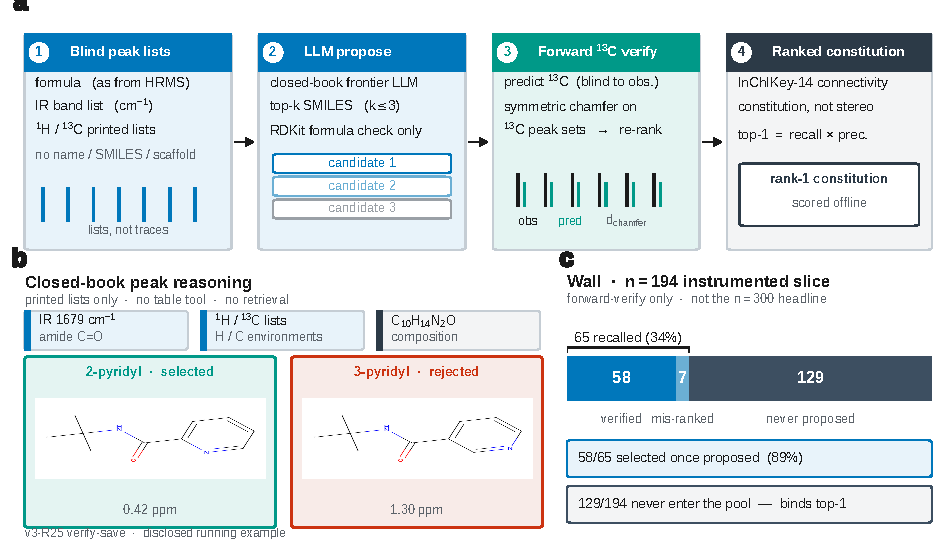
\includegraphics[width=\linewidth]{fig1_overview.pdf}
  \caption{IRSpectra-Bench protocol.
  (a)~Printed IR/$^1$H/$^{13}$C lists $+$ formula $\rightarrow$ closed-book LLM
  proposes top-$k$ SMILES (RDKit formula check) $\rightarrow$ forward $^{13}$C
  (blind) $\rightarrow$ chamfer re-rank $\rightarrow$ InChIKey-14.
  (b)~Evidence is the lists themselves (no peak-table tool, no retrieval).
  Running example v3-R25 (IR 1679~cm$^{-1}$; chamfer 0.42 vs 1.30~ppm).
  (c)~Locked $n{=}194$ instrumented wall: 58 verified / 7 mis-ranked / 129 never
  proposed. \textbf{Not} a pooled $n{=}300$ wall
  (headline generation: Table~\ref{tab:headline}; diagnostic repeat:
  Figure~\ref{fig:fig-wall}).}
  \label{fig:fig1}
\end{figure}

\section{Related work}
\label{sec:related-work}

\paragraph{Trained spectra $\to$ structure models.}
Sequence and graph decoders on paired
corpora~\citep{chacko2024spectro,hu2024multitask,yang2026nmrtrans,ottomano2025nmiracle,alberts2024ir,alberts2025benchmarks}
are accurate in-distribution but typically scored end-to-end.
We do not claim to beat them on IRSpectra-Bench; Spectro, NMIRacle, Alberts IR transformers
and CASE are \textbf{not yet scored} on our bench (Section~\ref{sec:limitations}) --- a gap we
state honestly and leave to the released scorer.

\paragraph{Agentic elucidation: three regimes.}
The contrast is the \textbf{setting and the stage split}, not a method scoreboard.
(i)~\emph{Tool-using lab agents} --- ChemCrow~\citep{mbran2024chemcrow},
Coscientist~\citep{boiko2023coscientist} --- show that LLMs can call instruments and
planners; they do not measure which elucidation stage binds.
(ii)~\emph{Spectrum-native agents} improve \emph{how} a model reads a spectrum or
re-ranks a \textbf{fixed} pool: tree-search~\citep{zhuang2025treesearch},
SpecMol~\citep{shen2025specmol}, Priessner \textit{et al.}~\citep{priessner2026reasoning},
NMR-Solver~\citep{jin2025nmrsolver}, NMRAgent~\citep{fang2026nmragent}.
Priessner already notes that re-ranking cannot recover a missing candidate; we measure
that failure at literature-peak-list scale.
SpectraLLM~\citep{su2025spectrallm} is a \textbf{fine-tuned} multi-spectral elucidator
on \textbf{simulated} corpora (QM9S DFT; Alberts USPTO multimodal) --- a different object
and a different training regime; we do not score it here.
IR-Agent~\citep{noh2025iragent} (ICLR 2026) is the closest concurrent multi-agent IR
elucidator: on \textbf{NIST experimental IR} a translator proposes a SMILES pool, TI+Ret
enrich local (peak-table) and global (retrieved-spectrum) features, and an SE expert
re-ranks (Top-$k$ SMILES; atom type / scaffold / carbon count may be prompt-injected).
(iii)~\emph{Agentic-search benches} --- MolQuest~\citep{han2026molquest},
NMRGym~\citep{fang2026nmrgym}, Espejo Morales \textit{et al.}~\citep{espejo2026agentic}
(education $\to$ industrial instrument files: 80.9\% $\to$ 20.6\%) --- ask which
architecture or abductive loop wins.
IRSpectra-Bench is the harder operational object: \textbf{literature peak lists}
(IR+$^1$H/$^{13}$C+formula as from HRMS), \textbf{off-the-shelf} closed-book models, no
name, SMILES, or scaffold hint.
We measure \textbf{which stage binds} after spectra are read --- generation recall versus
verification precision $|$ recall --- on pooled $n{=}300$, with instrumented
forward-verify on $n{=}194$.
IR-Agent's SE expert over a \textbf{fixed candidate pool} is exactly the regime our
ladder diagnoses as recall-limited (proposal binds; conditional forward-verify
$\approx$89\%, 58/65).
TI+Ret can enrich \emph{features} but does \textbf{not} remove a proposal wall if the true
structure never enters the pool.
Architecture search that does not change $P(\text{true}\in\text{pool})$ cannot move
top-1 on a recall-bound bench.
We do not claim to beat SpectraLLM or IR-Agent on their native sets; neither is scored
here.
\begin{center}
\scriptsize
\setlength{\tabcolsep}{4pt}
\begin{tabular}{@{}llll@{}}
\toprule
 & input & metric & binds \\
\midrule
IR-Agent & NIST experimental IR & Top-$k$ SMILES & re-rank given pool \\
this paper & lit.\ IR+$^1$H/$^{13}$C+formula lists & recall vs prec.$|$recall & proposal \\
\bottomrule
\end{tabular}
\end{center}

\paragraph{Heterogeneous data, CASE, and positioning.}
Most prior suites use simulated or single-instrument spectra; we use literature-reported
peak lists across thousands of laboratories and report formula-only and recency controls
(Section~\ref{sec:contamination}).
Matching predicted to observed shifts --- DP4~\citep{smith2010dp4},
CASE~\citep{elyashberg2012case}, NMR-Solver, NMRAgent --- is easier than inverse
generation; CASE enumerators have exhaustive recall by construction, while the LLM
literature almost never reports whether the true structure was proposed at all.
SpecX~\citep{xiang2026specx} bounds a related multi-modal spectroscopy task on
simulated traces.
IRSpectra-Bench is an openly redistributable literature-peak-list suite with a
\textbf{stage decomposition}, measured on Claude and replicated across three other
model families.

\FloatBarrier
\section{IRSpectra-Bench}
\label{sec:benchmark}

\subsection{Task and inputs}

Each of 300 problems supplies the \textbf{molecular formula} (as from HRMS), the \textbf{IR
band list} (cm$^{-1}$), and \textbf{$^1$H / $^{13}$C shift lists} --- exactly the textual form
reported in open-access papers.
No name, SMILES or scaffold hint.
Inputs are author-transcribed \textbf{band and shift lists}, not absorbance traces or FIDs:
a different object from digitised-spectrum benchmarks~\citep{espejo2026agentic}, and one that
matches how language models consume literature.

The cohort is the pre-registered pool of a locked 194 (spectrally validated main round 134 $+$
60 controls) and a 106-compound expansion draw ($n{=}300{=}194{+}106$).
Five expansion records fail the same $^{13}$C-overread audit used on the main round and are
included in the 300 (validate-clean $n{=}295$ in Appendix~\ref{app:extended}).
Problems are drawn from the structure-complete split of IRexp (\texttt{irexp\_resolved}; see
companion Data Descriptor)~\citep{yabbarov2026irexp}.
On the locked 194, author peak assignments name a ring system in 10/194; those are solved
1/10 vs 54/184 for the rest, so named-ring annotation does not drive that slice.
Figure~\ref{fig:fig-chemspace} summarises the chemistry space of the pooled headline.
Figure~\ref{lst:payload} is the solver-facing contract: formula plus printed peak lists,
gold constitution held out.

\begin{figure}[ht]
  \centering
  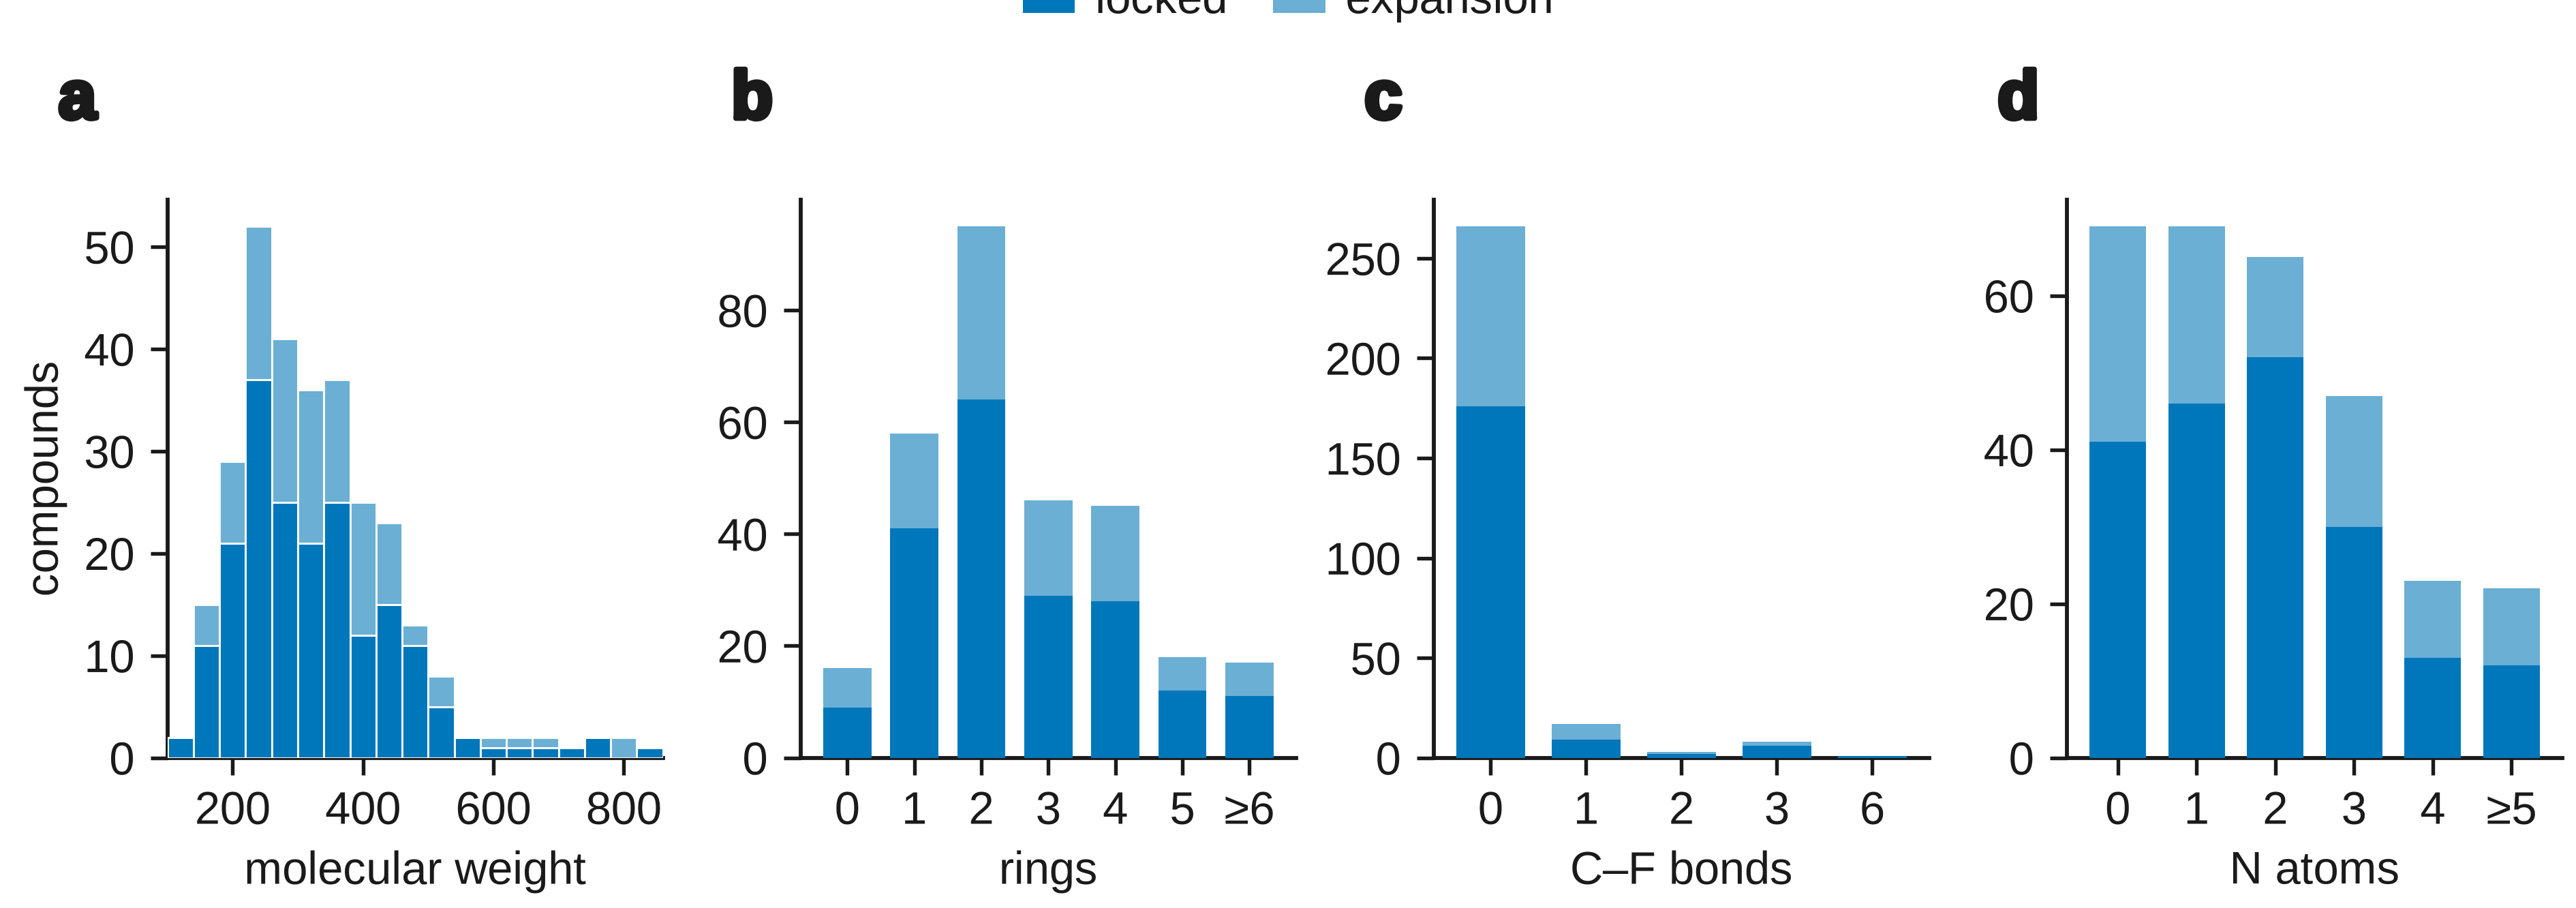
\includegraphics[width=0.92\linewidth]{fig_chemspace.png}
  \caption{Pooled headline chemistry ($n{=}300$; panels on validate-clean $n{=}295$).
  (a)~MW (median 306). (b)~RDKit rings (median 2). (c)~C--F bonds. (d)~N atoms.
  Stacked: locked (dark) vs expansion (light). Mid-size literature space, not a NIST toy set.}
  \label{fig:fig-chemspace}
\end{figure}

\subsection{Difficulty, balance, and scoring contract}

\textbf{Difficulty} is declared \emph{a priori} by RDKit ring analysis: \emph{simple} iff
$\leq$2 rings, no fused/spiro/bridgehead system, $\leq$22 heavy atoms; else \emph{complex}
(151/149 on $n{=}300$).
The released benchmark is \textbf{50/50 by design}; the eligible corpus is 17.5\% simple /
82.5\% complex.
Reweighted to corpus composition on the validate-clean subset, top-1 falls 39.3\% $\to$
\textbf{26.5\%} [21--32] and recall 44.1\% $\to$ \textbf{31.3\%} [25--37]
(Appendix~\ref{app:extended}).
We report both: the reweighted figure is the better estimate for an arbitrary paper, and the
50/50 figure is the comparable leaderboard number (Table~\ref{tab:headline}).

\textbf{Scoring.} A prediction is correct if RDKit InChIKey \textbf{connectivity} (first 14
characters) matches --- we score \emph{constitution}.
Full stereo-sensitive InChIKey is reported on the validate-clean subset
(Appendix~\ref{app:extended}).
External submissions: up to three ranked SMILES per \texttt{qid}, no structure hints
(\texttt{docs/LEADERBOARD.md}; \texttt{scripts/score\_submission.py}).
Primary metrics (report all three): \textbf{top-1} (best-ranked candidate matches at
connectivity); \textbf{generation recall} (reference in the pool \emph{before} re-ranking);
\textbf{verification precision $|$ recall} (correct top-1 among recall-positive compounds).
Confidence intervals are bootstrap 95\%; paired model differences use McNemar with Holm correction.

\section{Experimental setup}
\label{sec:setup}

\paragraph{Blind payload and solver.}
The solver sees four JSON fields per \texttt{qid}: \texttt{formula} (as from HRMS),
\texttt{ir\_bands\_cm-1}, \texttt{h\_nmr}, \texttt{c\_nmr} --- peak lists as printed
(Figure~\ref{lst:payload}).
No name, SMILES, scaffold, atom-type hint, or retrieved spectrum; ground truth is scored
offline.
Frontier LLM agent (Claude Opus via consumer subscription), closed-book, one sub-agent per
batch, RDKit formula check only.
No fine-tuning, no paid API, \textbf{no thinking tier} for the core protocol.
Inference is \textbf{not} exactly reproducible (no pinned snapshot, temperature or seed ---
Section~\ref{sec:limitations}).
\textbf{Scoring is reproducible}: frozen predictions, ground truth and scorers regenerate every
training-free number.

\begin{figure}[ht]
\centering
\begin{minipage}{0.98\linewidth}
\begin{framed}
\noindent
\begin{minipage}[c]{0.56\linewidth}
\begin{lstlisting}[style=benchjson]
{
  "qid": "v3-R25",
  "formula": "C10H14N2O",
  "ir_bands_cm-1": [1679, "..."],
  "h_nmr": "[printed 1H list]",
  "c_nmr": "[printed 13C list]"
}
\end{lstlisting}
\end{minipage}\hfill
\begin{minipage}[c]{0.40\linewidth}
\centering
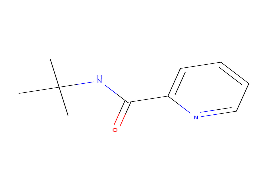
\includegraphics[width=\linewidth]{fig_listing_mol.pdf}\\[0.2em]
{\scriptsize\itshape gold held out}\\[-0.1em]
{\scriptsize 2-pyridyl picolinamide}
\end{minipage}
\end{framed}
\end{minipage}
\caption{\textbf{Listing 1.} Solver-facing payload (abridged), IRexp
JSON$+$molecule layout. Gold constitution (right) is held out.
Only disclosed fragments are shown (v3-R25 / C$_{10}$H$_{14}$N$_{2}$O / IR 1679);
full lists ship with the bench. Source: IRexp~\citep{yabbarov2026irexp};
this PDF is not a Data Descriptor.}
\label{lst:payload}
\end{figure}

\paragraph{Scoring contract and candidate budget.}
A deposit is JSONL of \texttt{\{qid, candidates: [SMILES,\ldots]\}} under a stated budget.
The scorer reports the three Section~\ref{sec:benchmark} metrics at InChIKey-connectivity,
with bootstrap 95\% CIs.
Self-ranking vs forward-verified re-ranking must be labelled; they are not interchangeable.
Headline protocol: $\leq$3 ranked SMILES per \texttt{qid}.
On the 60-compound arm Claude returned mean 2.20 candidates vs 3.00 for the other vendors
(recall rankings approximate).
\textbf{Generate-wide} (that arm only): ten independent solvers $\times$ up to six SMILES,
pooled then re-ranked --- not the $n{=}300$ reporting budget.

\paragraph{Forward-verification, expansion, and probes.}
Generate $\to$ forward-predict $^{13}$C (blind to the observed list) $\to$ re-rank by
symmetric chamfer on $^{13}$C peak sets (Section~\ref{sec:forward-verify}); instrumented on
the locked $n{=}194$ only.
Expansion is a pre-registered 106-compound draw from the same \texttt{irexp\_resolved}
sampler after the $n{=}194$ lock, with the same $^{13}$C-overread audit
(Section~\ref{sec:expansion}): five flags stay in the $n{=}300$ headline; validate-clean
$n{=}295$ is appendix; expansion-106 forward-verify was not run.
A later 230-compound draw toward $n{\approx}500$ is deposited and unscored
(Section~\ref{sec:expansion}).
Controls: formula-only / recency (Section~\ref{sec:contamination}); four-vendor replication
on a 60-compound arm (Section~\ref{sec:cross-vendor}); generate-wide sampling; HOSE lookup
and GNN $^{13}$C verifiers; small IRexp-fine-tuned generator probe (excluded from headline
claims).

\section{Results}
\label{sec:results}

\subsection{Headline performance}
\label{sec:headline}

\begin{table}[ht]
\caption{Headline elucidation ($n{=}300{=}194$ locked $+$ $106$ expansion).
Bootstrap 95\% CIs; validate-clean $n{=}295$ in Appendix~\ref{app:extended}.}
\label{tab:headline}
\centering
\small
\begin{tabular}{@{}lr@{}}
\toprule
metric & $n{=}300$ \\
\midrule
top-1 exact constitution & \textbf{39.3\%} (118/300) [34--45] \\
\quad simple ($n{=}151$) & 58.3\% (88/151) \\
\quad complex ($n{=}149$) & 20.1\% (30/149) \\
generation recall (top-3) & \textbf{44.3\%} (133/300) [39--50] \\
\bottomrule
\end{tabular}
\end{table}

On the validate-clean subset, scaffold-level recovery is 64\% (simple 80\%, complex 48\%) and
mean best Tanimoto is 0.66; accuracy falls with size (67.9\% top-1 at $\leq$15 heavy atoms,
42.8\% at 16--25, 16.7\% above 25; $n{=}53/152/90$; Appendix~\ref{app:extended}).
On the locked 194, of 137 analysable top-1 misses, \textbf{76.6\%} are constitutional isomers of the true
structure; only \textbf{22.6\%} share the true Murcko scaffold --- wrong connectivity at the
right composition, not mostly fine regiochemistry (not re-run on the expansion).
A 24-compound four-model Claude comparison is capability-sensitive (Haiku $\subset$ Sonnet
$\subset$ Opus $\subset$ Fable) but underpowered for adjacent ranks, with a disclosed protocol
asymmetry (Section~\ref{sec:limitations}); a battery-electrolyte subset ($n{=}46$) matches the
locked-slice regime (26\% top-1; recall-bound).

\begin{table}[ht]
\caption{Generation by slice. Headline is pooled $n{=}300$, not locked 194 alone.}
\label{tab:slices}
\centering
\small
\begin{tabular}{@{}lrrr@{}}
\toprule
 & locked ($n{=}194$) & expansion ($n{=}106$) & pooled ($n{=}300$) \\
\midrule
top-1 & 55/194 (28.4\%) & 63/106 (59.4\%) & \textbf{118/300 (39.3\%)} \\
generation recall & 65/194 (33.5\%) & 68/106 (64.2\%) & \textbf{133/300 (44.3\%)} \\
\bottomrule
\end{tabular}
\end{table}

The expansion slice is easier for this solver than the locked 194 (59.4\% vs 28.4\% top-1);
pooling does not hide that gap.
Self-ranking precision $|$ recall on the pooled generation cohort is 118/133 (88.7\%) ---
that is \emph{not} forward-verification precision (Section~\ref{sec:forward-verify}).

\subsection{Is the model reading the spectra?}
\label{sec:contamination}

\begin{table}[ht]
\caption{Formula-only control (paired, $n{=}60$).}
\label{tab:formula-only}
\centering
\small
\begin{tabular}{@{}lrr@{}}
\toprule
condition & top-1 & recovered (top-3) \\
\midrule
formula only & \textbf{3/60 (5\%)} & 3/60 (5\%) \\
formula + IR + $^1$H + $^{13}$C & 14/60 (23\%) & 19/60 (32\%) \\
\bottomrule
\end{tabular}
\end{table}

Outcomes are perfectly nested (McNemar $p{=}0.001$).
Accuracy is flat in source-paper year across the locked 194 ($r{=}{-}0.007$), bounding pretraining
recall of specific papers.
We claim a \textbf{strong bound, not exclusion} of contamination
(Section~\ref{sec:limitations}).

\begin{figure}[ht]
  \centering
  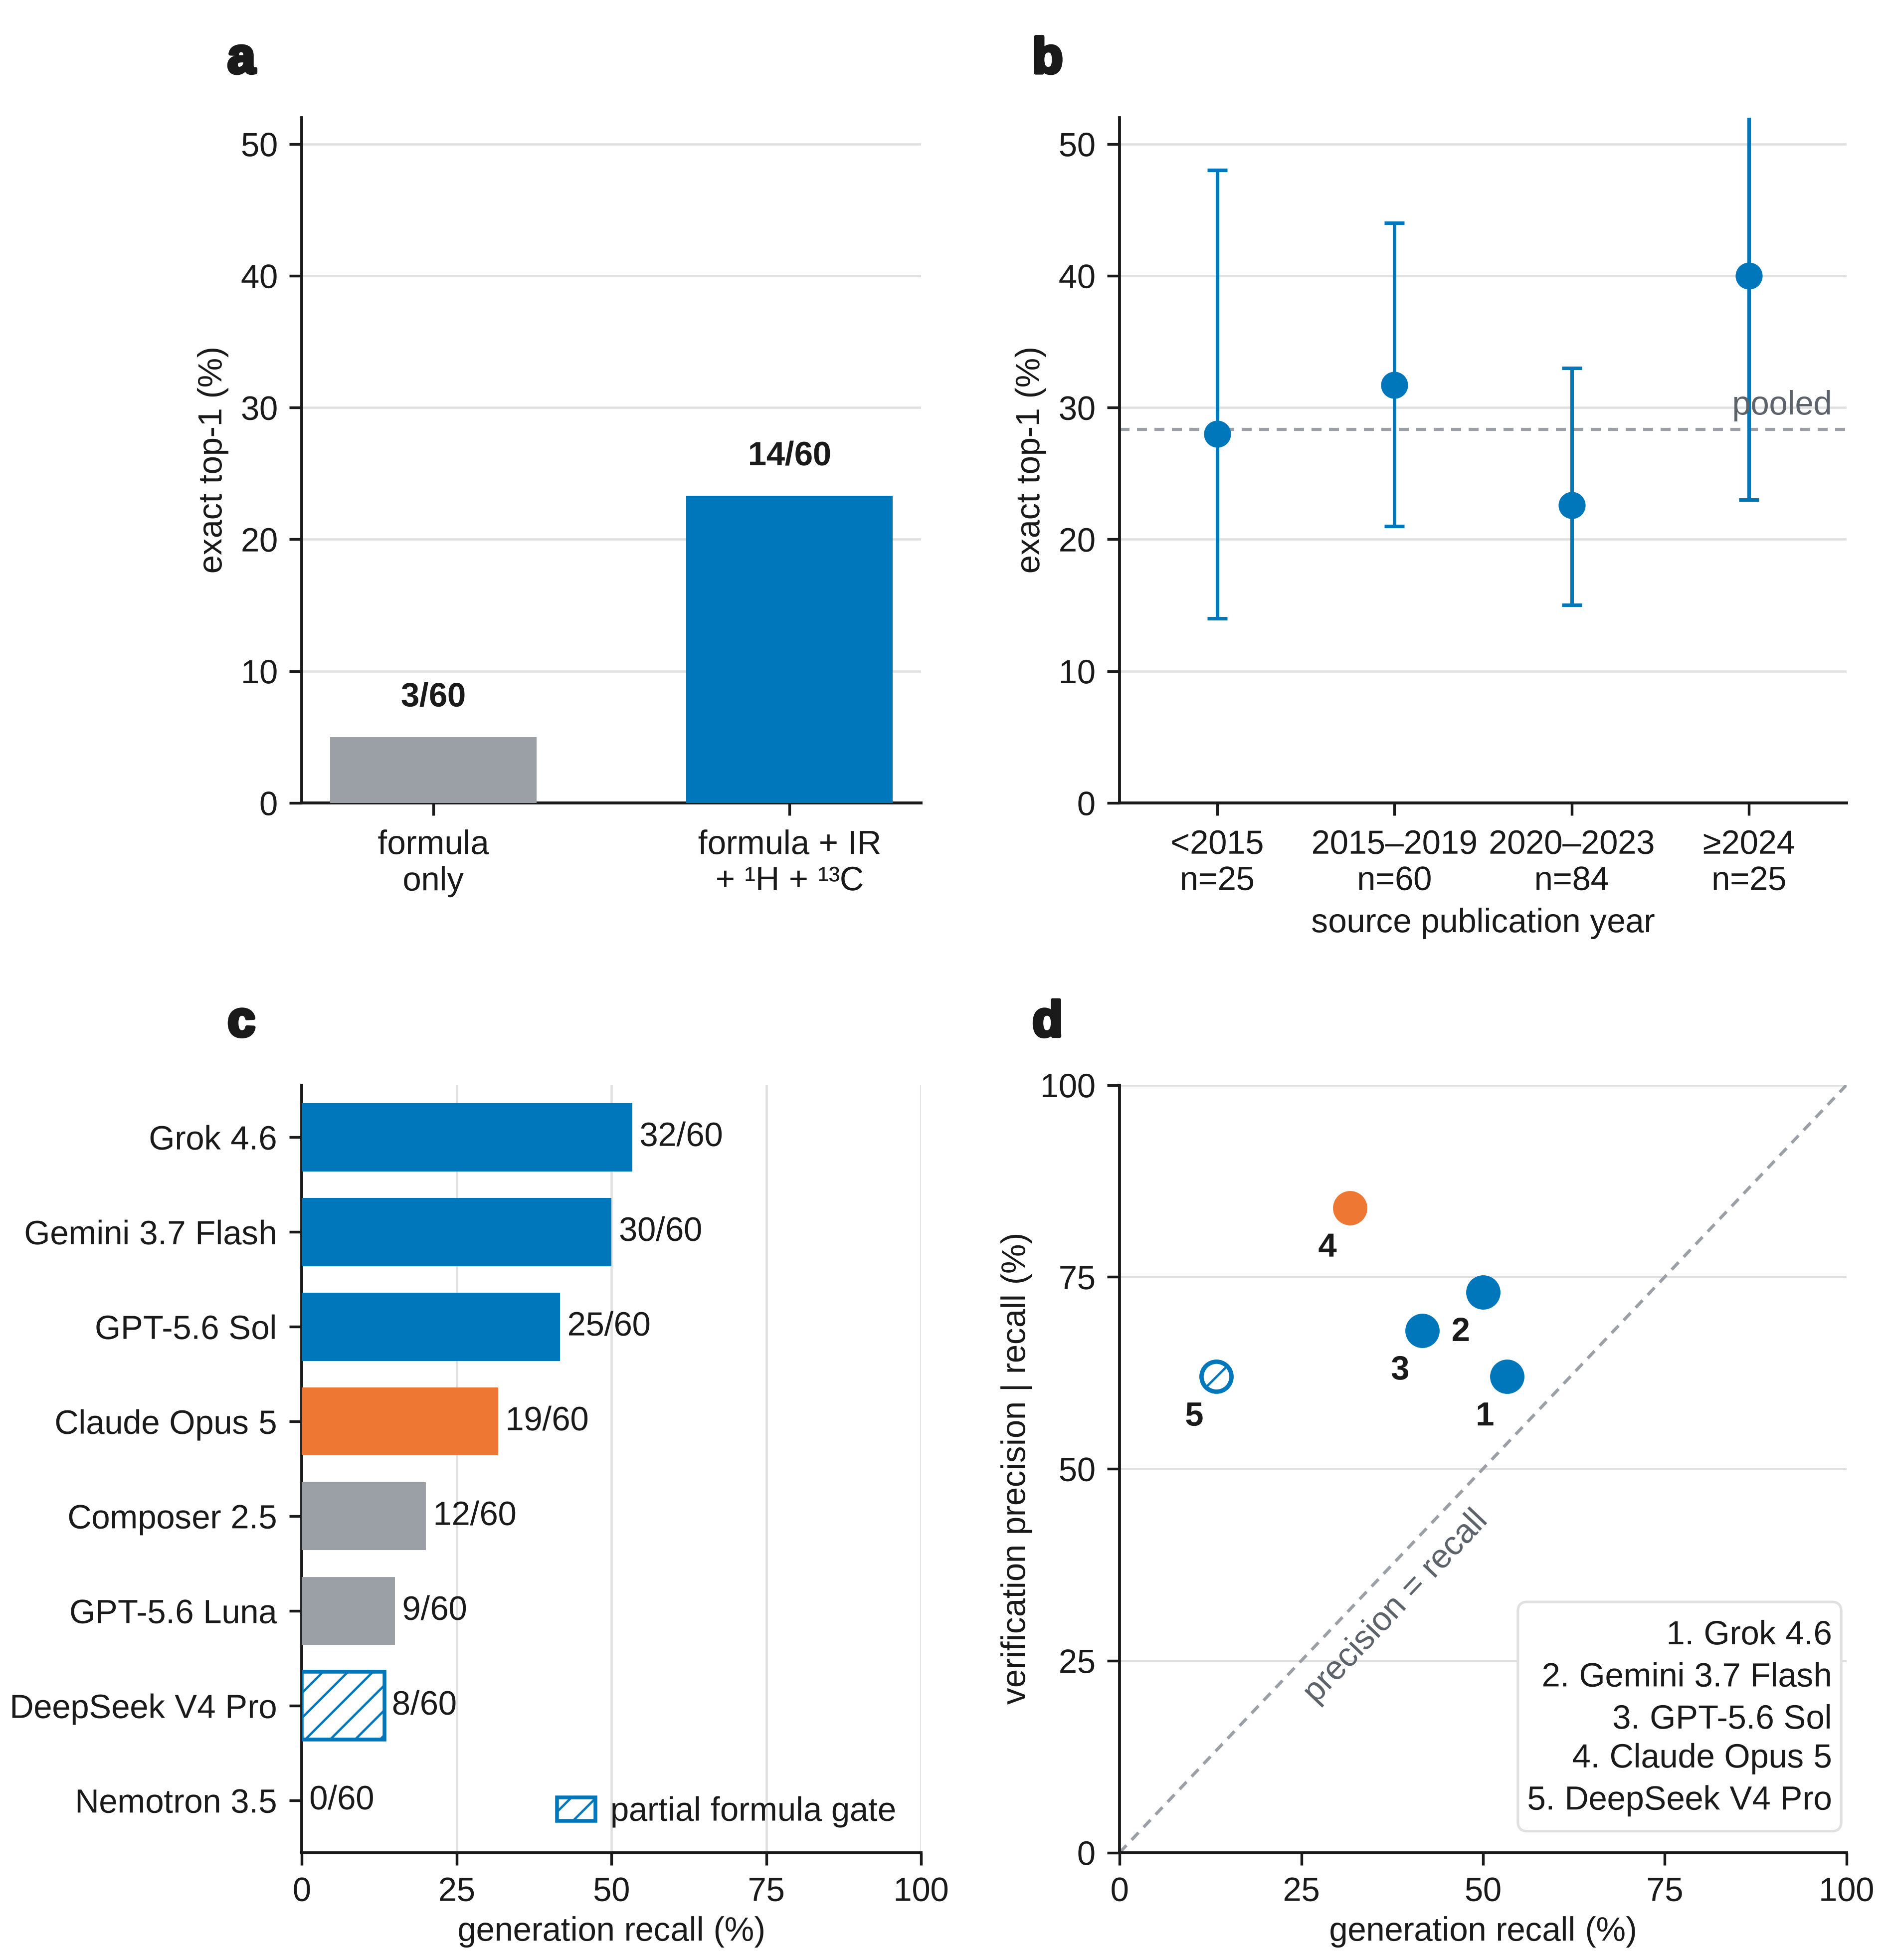
\includegraphics[width=0.62\linewidth]{fig_robustness.png}
  \caption{Robustness on instrumented arms (formula-only / cross-vendor $n{=}60$;
  recency $n{=}194$): formula-only collapse, flat recency, four-vendor recall $\ll$ precision.}
  \label{fig:fig-robustness}
\end{figure}

\subsection{Cross-vendor replication}
\label{sec:cross-vendor}

Grok 4.6, Gemini 3.7 Flash and GPT-5.6 Sol solved the same 60-compound arm under the
identical protocol.
\textbf{Verification precision exceeds generation recall in every arm}; bootstrapping
separates the paired gap for Claude (+52.5 points), GPT-5.6 Sol (+26.3) and Gemini (+23.3);
Grok's gap (+9.2) is directional.

\begin{table}[ht]
\caption{Cross-vendor decomposition ($n{=}60$). Recall and precision use different denominators.}
\label{tab:cross-vendor}
\centering
\small
\begin{tabular}{@{}lrrr@{}}
\toprule
model & generation recall & verification precision $|$ recall & multi-candidate only \\
\midrule
Claude Opus & 19/60 = 32\% & 16/19 = 84\% & 10/13 = 77\% \\
Grok 4.6 & 32/60 = 53\% & 20/32 = 62\% & 20/32 = 62\% \\
Gemini 3.7 Flash & 30/60 = 50\% & 22/30 = 73\% & 22/30 = 73\% \\
GPT-5.6 Sol & 25/60 = 42\% & 17/25 = 68\% & 16/24 = 67\% \\
\bottomrule
\end{tabular}
\end{table}

Candidate budgets differ (Claude mean 2.20 vs others 3.00), so recall rankings are
approximate.
A clean-clone control for Grok bounds key leakage (McNemar $p{=}0.39$).

\subsection{Forward-verification decomposition}
\label{sec:forward-verify}

\begin{figure}[ht]
  \centering
  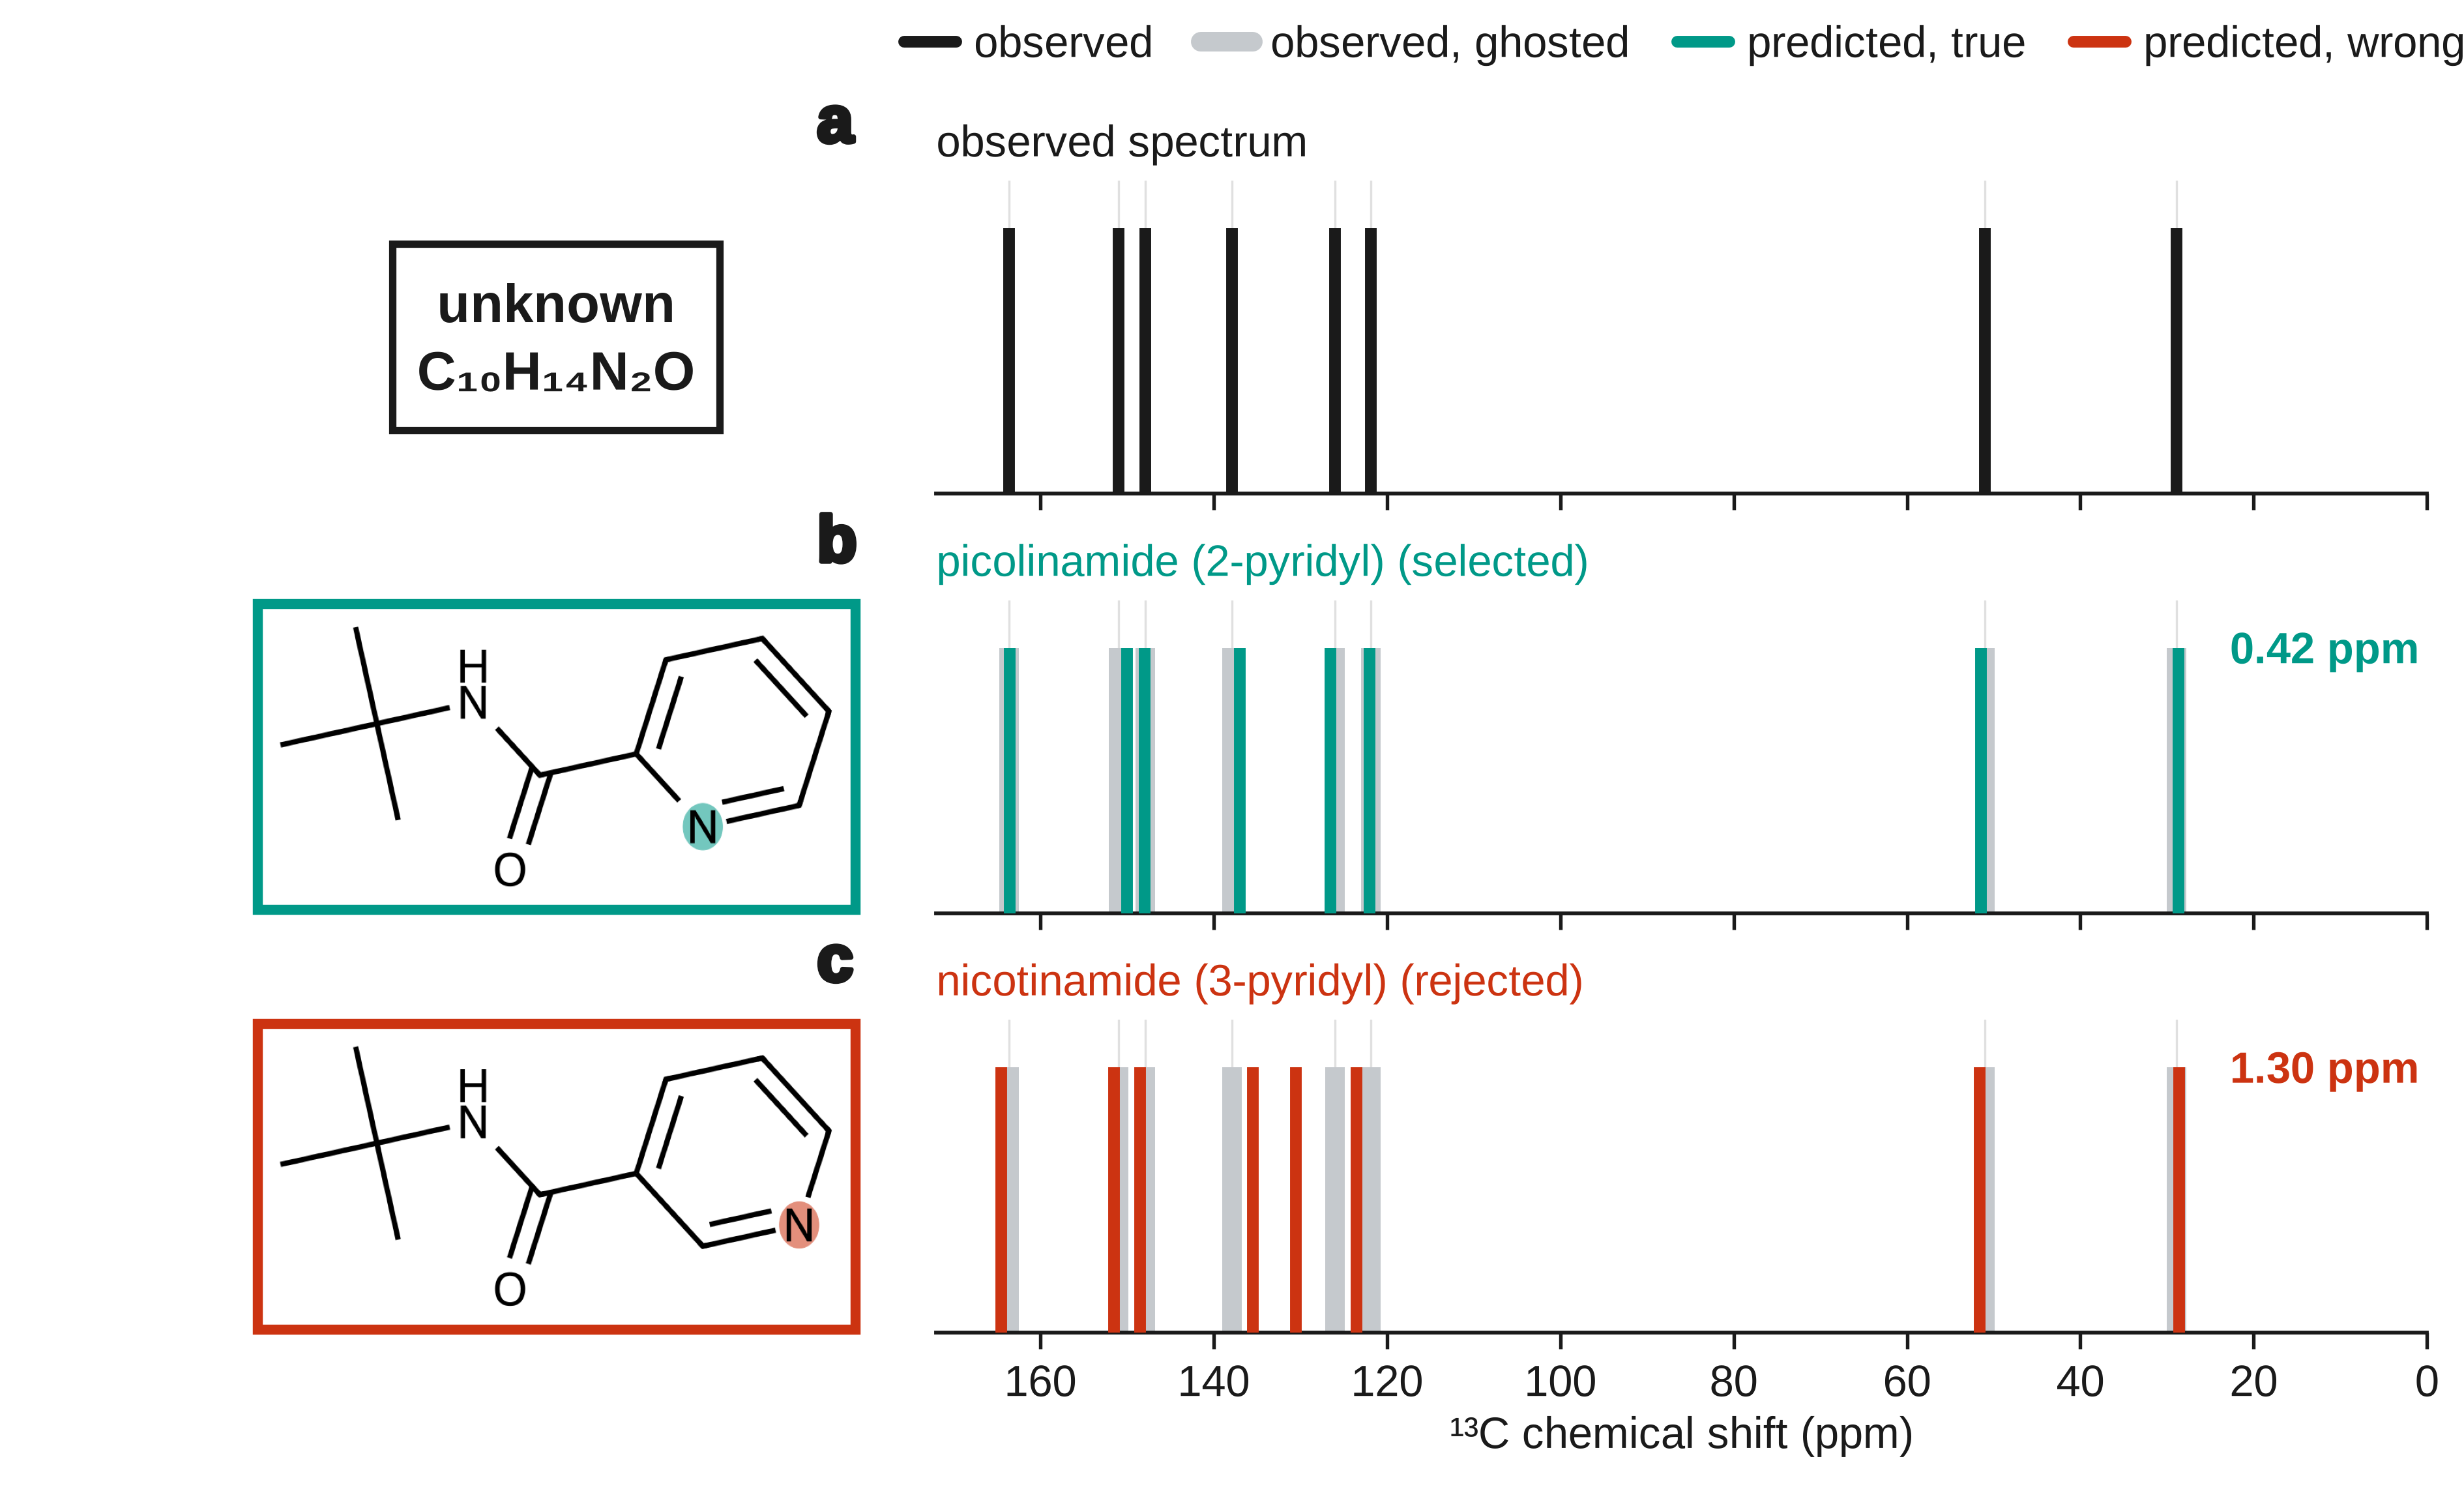
\includegraphics[width=0.72\linewidth]{fig_mechanism.png}
  \caption{Locked v3-R25: self-rank prefers 3-pyridyl; forward $^{13}$C recovers 2-pyridyl
  (chamfer 0.42 vs 1.30~ppm) --- a verify-save, not a recall win (Table~\ref{tab:cases}).}
  \label{fig:fig-mechanism}
\end{figure}

\begin{table}[ht]
\caption{Forward-verify on the instrumented slice ($n{=}194$).
Pooled $n{=}300$ in Table~\ref{tab:headline} is generation only.}
\label{tab:fverify}
\centering
\small
\begin{tabular}{@{}lrr@{}}
\toprule
 & 60-compound arm & locked slice ($n{=}194$) \\
\midrule
generation recall & 19/60 (32\%) & 65/194 (34\%) \\
top-1, solver self-ranking & 14/60 (23\%) & 55/194 (28\%) \\
top-1, forward-verified re-ranking & 16/60 (27\%) & 58/194 (30\%) \\
precision $|$ recall --- forward-verification & 16/19 (84\%) & 58/65 (\textbf{89\%}) \\
multi-candidate only --- forward-verification & 10/13 (77\%) & 30/37 (81\%) \\
\bottomrule
\end{tabular}
\end{table}

When the true structure is among the candidates, forward-verification selects it in 58/65
cases (89\%).
Where a choice existed ($n{=}37$), forward-verification is correct on 30/37 (81\%) against a
54.0\% derangement floor (+27.1 points).
The margin over self-ranking is \textbf{small and unresolved} (seven gained, four lost;
McNemar $p{=}0.55$) --- we do \textbf{not} claim an accuracy advance.
Precision is high while recall binds: no re-ranking repairs the 129/194 compounds on this
slice where the true structure was never proposed (Figure~\ref{fig:fig1}c;
diagnostic repeat in Figure~\ref{fig:fig-wall}).

\paragraph{Worked cases.}
Three locked-slice deposits instantiate the wall (Appendix Table~\ref{tab:cases}; expansion
qids reuse R22/R25 --- IDs below are locked-round labels).
\textbf{main-R06} (C$_{29}$H$_{30}$FNO$_{2}$): true acridinedione never enters the 3-candidate
pool (Tanimoto-0.90 regioisomer); verifier unused.
\textbf{v3-R25} (C$_{10}$H$_{14}$N$_{2}$O): verify-save --- self-rank prefers 3-pyridyl,
forward $^{13}$C recovers 2-pyridyl (chamfer 0.42 vs 1.30~ppm; Figure~\ref{fig:fig-mechanism}).
\textbf{v3-R26} (C$_{14}$H$_{11}$N$_{3}$O$_{3}$): verify-fail --- true 3-nitrophenyl isomer in
the pool but 2-nitro ranked first (chamfer 1.35 vs 1.36~ppm).

\paragraph{Generate-wide.}
Ten solver agents, up to six candidates each, pooled and re-ranked on the 60-compound arm:
recall 32\% $\to$ \textbf{42\%}, top-1 23\% $\to$ \textbf{30\%} (McNemar $p{=}0.34$);
verification precision falls 84\% $\to$ 72\%.
The training-free ceiling remains recall-limited.

\begin{figure}[ht]
  \centering
  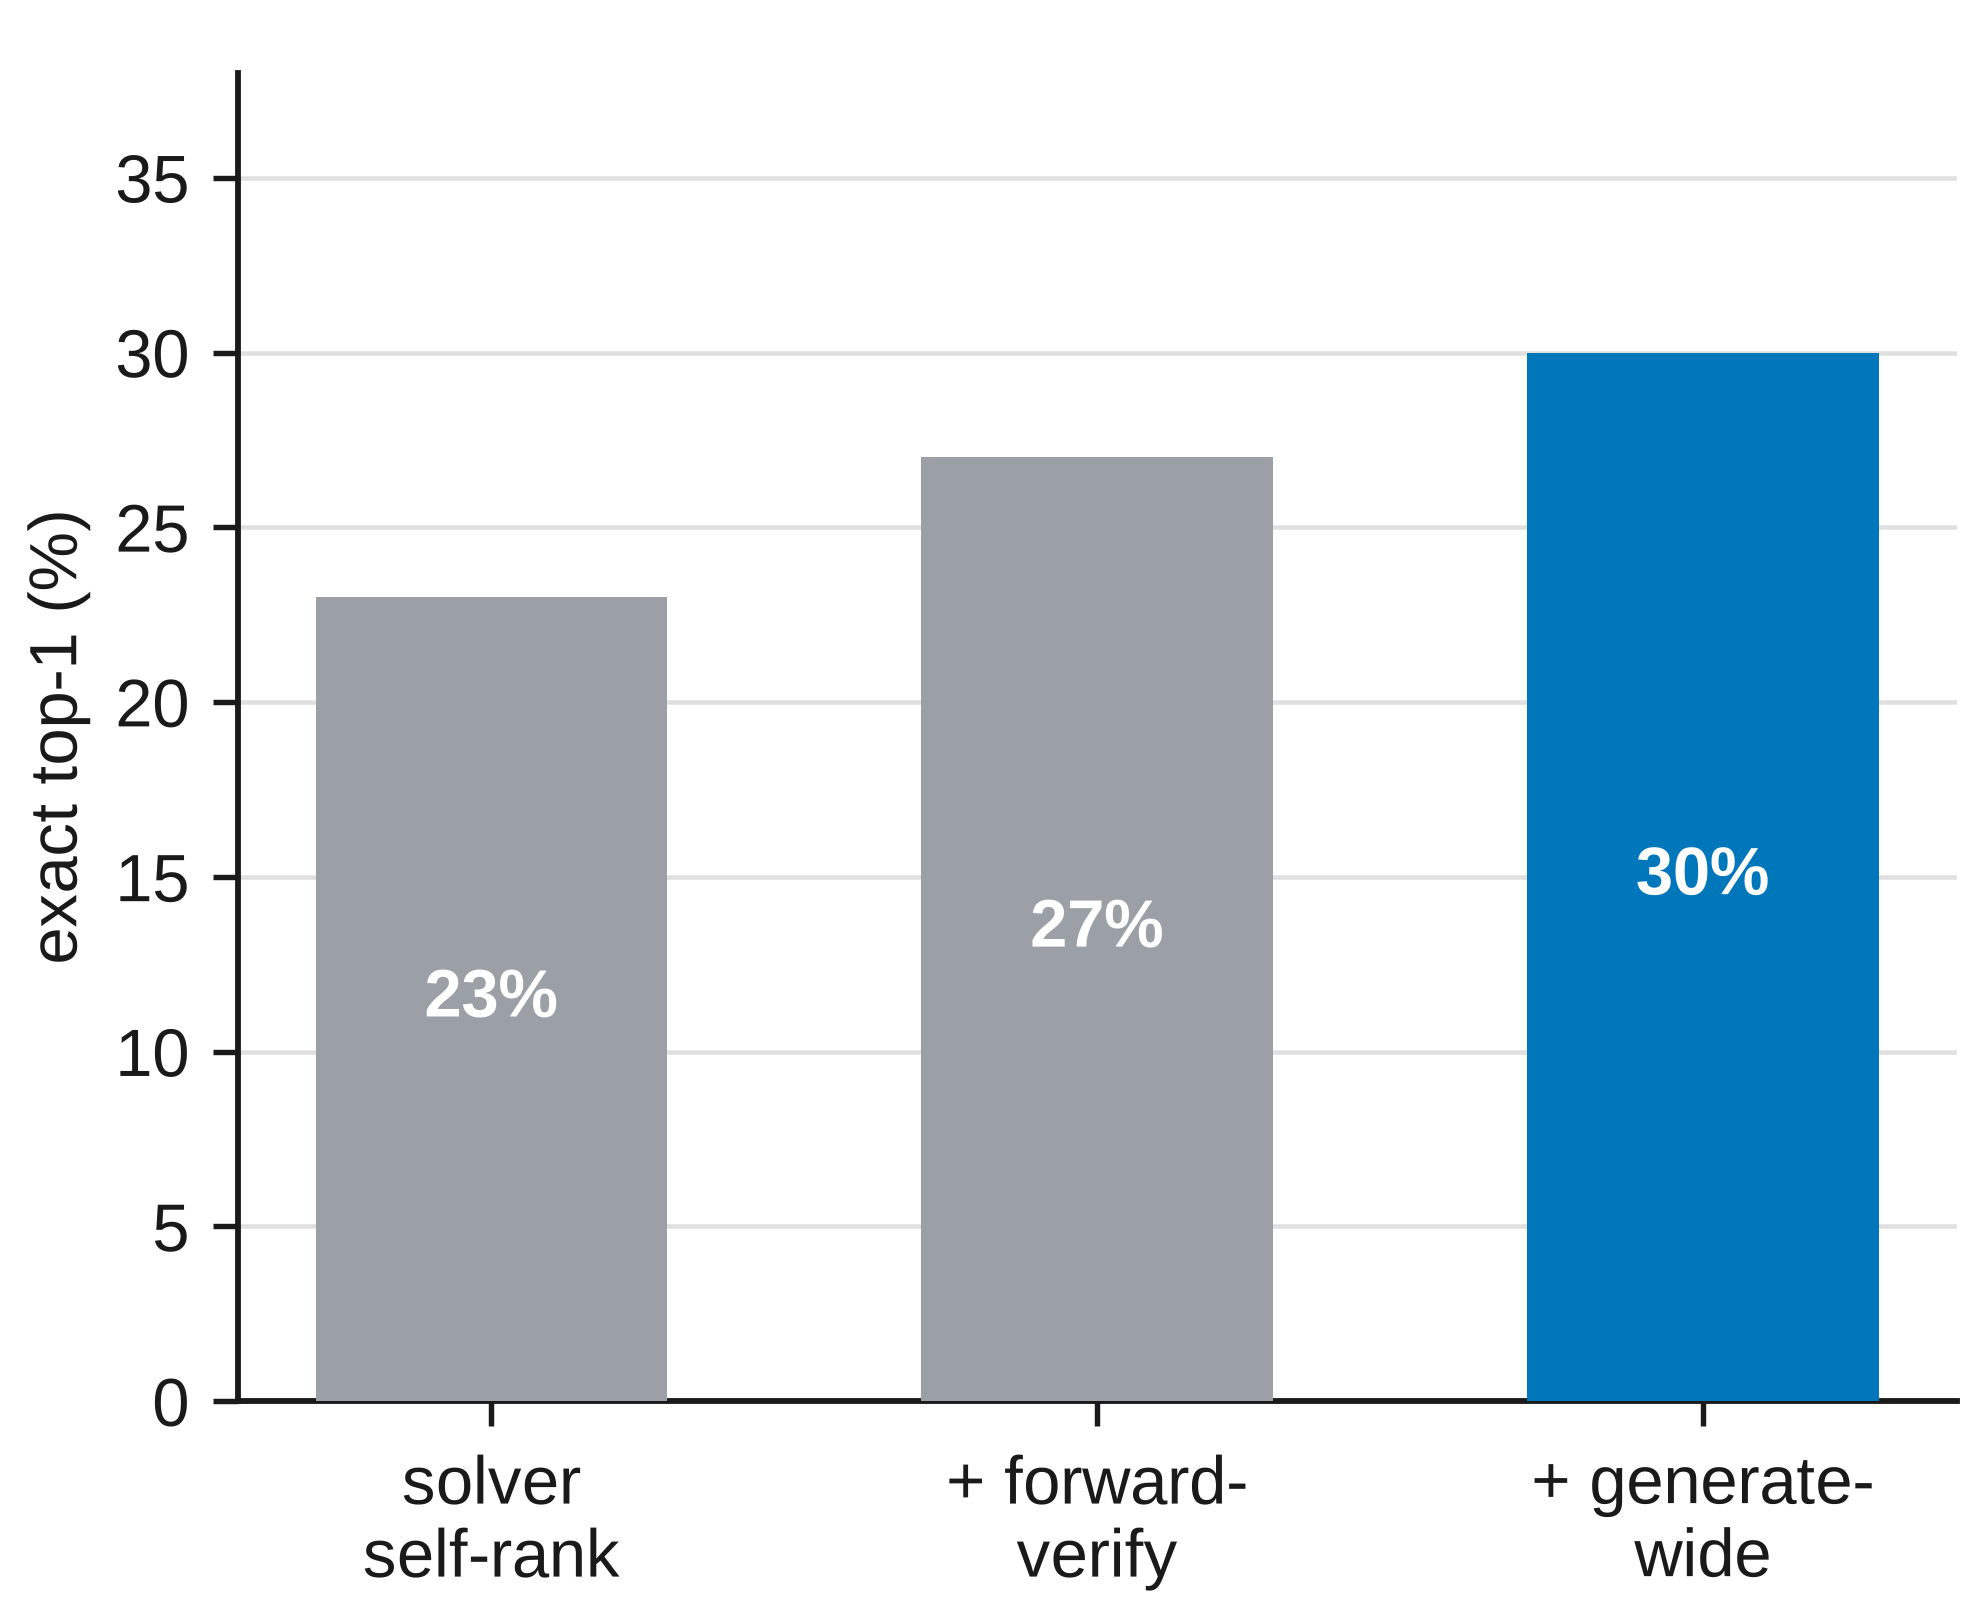
\includegraphics[width=0.52\linewidth]{fig3_method.png}
  \caption{Inference ladder on the 60-compound arm: 23\% $\to$ 27\% $\to$ 30\% top-1.
  Generate-wide lifts recall (32\% $\to$ 42\%); the wall is proposal, not ranking.}
  \label{fig:fig3-method}
\end{figure}

\paragraph{Non-LLM verifiers.}
On the same candidate sets, a HOSE-style lookup ties self-ranking; a modest GNN reaches
59/65 (91\%) vs the LLM verifier's 58/65 (89\%) --- directional.
Deranging observed $^{13}$C pairings collapses precision ($p{=}0.001$).
A small IRexp-fine-tuned generator pooled with Claude lifts locked-slice recall 33.5\% $\to$ 54.1\% and
top-1 28.4\% $\to$ 35.1\% (McNemar $p{=}0.015$), showing the wall is a property of
\textbf{training-free elicitation}, not of the task.

\subsection{Decomposition across published literature}
\label{sec:literature}

Any system reporting top-1 $= a$ and top-$k = b$ implies recall $\geq b$ and conditional
precision $\leq a/b$.
Applying this to published figures (\texttt{scripts/literature\_decomposition.py}):

\begin{table}[ht]
\caption{Selected literature decomposition rows (connectivity-scored or as published).}
\label{tab:lit-decomp}
\centering
\scriptsize
\setlength{\tabcolsep}{3pt}
\begin{tabular}{@{}p{2.6cm}p{2.4cm}rrrr@{}}
\toprule
system & data ($n$) & top-1 & top-$k$ ($k$) & recall & prec. \\
\midrule
this work, solver alone & literature (300) & 39.3\% & 44.3\% (3) & 44.3\% & 88.7\% \\
this work + forward-verify & literature (194) & 29.9\% & 33.5\% (3) & 33.5\% & \textbf{89.2\%} \\
NMR-Solver~\citep{jin2025nmrsolver} & literature (450) & 52.9\% & 67.3\% (10) & $\geq$67.3\% & $\leq$78.6\% \\
NMRAgent~\citep{fang2026nmragent} & literature (450) & 61.6\% & 70.0\% (10) & $\geq$70.0\% & $\leq$88.0\% \\
Espejo Morales~\citep{espejo2026agentic} & education (236) & 80.9\% & 90.0\% (5) & $\geq$90.0\% & $\leq$89.9\% \\
Espejo Morales~\citep{espejo2026agentic} & industrial (34) & 20.6\% & 29.1\% (5) & $\geq$29.1\% & $\leq$70.9\% \\
Alberts, 6--13 atoms~\citep{alberts2025benchmarks} & NIST IR (3,455) & 63.8\% & 84.0\% (10) & 84.0\% & 75.9\% \\
SpecX, scaffold split~\citep{xiang2026specx} & simulated (99,439) & 29.7\% & 50.6\% (10) & 50.6\% & 58.7\% \\
\bottomrule
\end{tabular}
\end{table}

\textbf{Three groups changed only the data}, and recall carried \textbf{68\%} (NMR-Solver
simulated $\to$ real), \textbf{70\%} (SpecX random $\to$ scaffold) and \textbf{83\%}
(Espejo education $\to$ industrial) of each collapse.
Recall binds where spectra are real and heterogeneous; ranking dominates on simulated or
single-library data.
The solver-alone precision column on $n{=}300$ is self-ranking (118/133); the
forward-verify row is the instrumented $n{=}194$ slice (58/65) --- not interchangeable.

\subsection{Pre-registered expansion, pooled headline, and scale roadmap}
\label{sec:expansion}

The $n{=}300$ headline is the pre-registered pool of the locked 194 and a 106-compound
expansion draw (Table~\ref{tab:slices}; Appendix Tables~\ref{tab:expansion},~\ref{tab:clean295}).
Five $^{13}$C-overread flags (R12, R22, R25, R82, R91) stay in the 300; validate-clean is
116/295 (39.3\%) top-1 / 130/295 (44.1\%) recall.
The expansion slice is easier (59.4\% vs 28.4\% top-1) --- disclosed, not hidden.
A Fable arm is incomplete (68/106; not scored; never pooled).
Figure~\ref{fig:fig-wall} and Table~\ref{tab:fverify} remain the $n{=}194$ instrumented
forward-verified diagnosis; expansion-106 fverify was \textbf{not} run.

\paragraph{Scale roadmap / larger blind round.}
A second pre-registered draw toward $n{\approx}500$ (230 compounds; 115/115 simple/complex;
six $^{13}$C-overread flags known \emph{before} any solve) now has \textbf{230/230} Opus
deposits and a frozen 690-candidate file.
Scoring is \textbf{deferred}: the answer key is withheld, no top-1 or recall exists, and
forward-verify was not run on this round.
Those deposits used a thinking-tier consumer arm and are not interchangeable with the
no-thinking $n{=}300$ protocol until scored under a declared contract.
This round is \textbf{not} pooled into the headline and is not a wall figure.

\section{Discussion}
\label{sec:discussion}

Frontier LLMs are \textbf{good verifiers} ($\approx$89\% conditional precision on the
$n{=}194$ instrumented slice) and \textbf{weak proposers} (44\% generation recall on
$n{=}300$; 34\% on the instrumented 194) on real literature peak lists --- propose $\gg$
verify, not the reverse.
The primary research contribution is the \textbf{benchmark + stage decomposition +
contamination/cross-vendor diagnosis}, not a solved elucidator and not a Data Descriptor
for IRexp.
The expansion slice scored higher than the locked 194 (Section~\ref{sec:expansion}); pooling
does not erase that gap.
The $n{\approx}500$ deposits do not yet change any scored number.

\paragraph{Reporting contract.}
External work on IRSpectra-Bench should deposit ranked SMILES under the released protocol and
report, at minimum: (i) top-1 constitution, (ii) generation recall, (iii) verification
precision $|$ recall, with bootstrap CIs and candidate budget.
Top-1 alone conflates the two stages.
Nonsignificant ladder gains (forward-verification vs self-ranking, $p{=}0.55$; generate-wide
top-1, $p{=}0.34$) should be cited as \textbf{diagnostic}, not as accuracy advances.
Corpus-reweighted top-1 (\textbf{26.5\%} on the validate-clean subset) is the better estimate
for an arbitrary literature draw.
Training is not foreclosed: IRexp fine-tuning lifts recall to 54\%.
Those gains compound with open experimental data, honest benchmarks, and inference scaffolding that
transfers to each new model.

\subsection{Implications for agentic elucidation}
\label{sec:agentic}

The diagnosis implies an \textbf{asymmetric pipeline}, not another verifier stacked on a thin
pool.
Proposal is the expensive stage: diversity, tool-use into enumeration / database search /
formula-constrained decode, or generate-wide sampling that actually enlarges the pool.
Verification is cheap: once the true constitution is proposed, training-free
forward-verification selects it $\approx$89\% of the time on the instrumented $n{=}194$
slice (58/65).
Spending the budget on a second ranker cannot recover the 129/194 compounds that were never
proposed.

IR-Agent-style table-interpretation and retrieve tools~\citep{noh2025iragent} are complementary
\emph{feature} agents --- they improve how a spectrum is read and how a given pool is
re-ranked.
MolQuest- and Espejo-style architecture search~\citep{han2026molquest,espejo2026agentic}
still needs this stage contract: a better reader that does not change
$P(\text{true}\in\text{pool})$ cannot move top-1 on a recall-bound bench.
The next ICLR-relevant agent is a \textbf{proposer}, not a second verifier:
formula-constrained generators, fragment assembly, and search that change that probability.
We are \textbf{not} shipping another ChemCrow-for-IR or a SpectraLLM-style fine-tune:
the bench is a reporting contract so external agents can be compared honestly on the same
object.
Multi-modal agents raise recall only if they enlarge the pool.
Training on open experimental corpora (IRexp as the pointer, not this paper's object) is the
one intervention we have already seen move recall (33.5\% $\to$ 54.1\% on the locked slice).
Nonsignificant ladder steps are \textbf{diagnostic}, not accuracy claims
(forward-verification vs self-ranking McNemar $p{=}0.55$; generate-wide top-1 $p{=}0.34$):
re-ranking is the wrong primary bet and does not license a solved-elucidator headline.

\section{Limitations}
\label{sec:limitations}

Scoring is mechanical; solver runs were transcript-audited for zero ground-truth access.
\textbf{(i) Consumer harness.} Claude Opus via consumer subscription; no model snapshot,
temperature, seed, or thinking tier. Exact inference is not reproducible; scoring is.
Batch instruction text was not captured --- only per-compound payloads are released.
We do \textbf{not} recommend thinking-high follow-ups as a path to a method result.
\textbf{(ii) Pretraining contamination} is bounded by formula-only (23\% $\to$ 5\%) and flat
recency but \textbf{not excluded}; verbatim spectral strings from PMC in the prompt remain a
retrieval confound.
\textbf{(iii) Object type, formula and scoring.} Band/shift lists, not raw traces; formula
supplied (as from HRMS) --- absolute accuracies are not interchangeable with no-formula
systems. Headline metrics score constitution; with stereochemistry, top-1 is 93/295 (31.5\%)
on the validate-clean subset.
\textbf{(iv) Statistical honesty.} Forward-verification vs self-ranking unresolved ($p{=}0.55$);
generate-wide top-1 likewise ($p{=}0.34$). Four-model comparison at $n{=}24$ underpowered for
adjacent ranks with disclosed protocol asymmetry. The inference ladder \textbf{diagnoses a
bottleneck}; it is not a demonstrated accuracy advance.
\textbf{(v) No method SOTA chase.} SpectraLLM, IR-Agent, Spectro, NMIRacle, Alberts IR
transformers and CASE were \textbf{not scored} on IRSpectra-Bench. The contribution is the
bench and the proposal$\ll$verification split, not a claim that an off-the-shelf LLM beats
trained elucidators.
\textbf{(vi) Expansion difficulty gap; fverify not on 106 or 230.} Expansion top-1 is 59\% vs 28\%
on the locked 194; pooling to $n{=}300$ does \textbf{not} hide that gap
(Table~\ref{tab:slices}). Figure~\ref{fig:fig-wall} and 58/65 are the locked $n{=}194$
instrumented slice; forward-verify was not run on the 106 or on the 230-compound
$n{\approx}500$ deposits. The $n{\approx}500$ round is deposited (230/230) and
\textbf{unscored} --- no top-1 --- and used a thinking-tier consumer arm, so it is not a
no-thinking replication. Headline $n{=}300$ is Claude Opus generation (no thinking
tier); four-vendor replication is on 60 compounds; candidate budgets differ.
A Fable expansion arm is incomplete (68/106) and is not pooled.
\textbf{(vii) Deferred arms.} Expert-chemist audit formally deferred (not run).
Leave-one-modality-out abandoned. Extraction-recall human audit of the mining parser is
deferred to the \textit{Scientific Data} companion.
\textbf{(viii) Scope.} Battery subset uses literature electrolyte chemistry, not operando
spectra; single-sample scoring per compound; organic literature bias of PMC-OA sources.
Short answers to the same attacks are collected in Appendix~\ref{app:faq}.

\section{Conclusion}
\label{sec:conclusion}

IRSpectra-Bench makes LLM structure elucidation from literature peak lists \textbf{measurable
and decomposable}.
On the pooled generation cohort ($n{=}300$), a frontier LLM recovers 39\% top-1 and 44\%
generation recall; corpus-reweighted top-1 is 27\%.
Propose $\gg$ verify: generation recall --- not verification --- binds end-to-end accuracy
(forward-verified on the locked $n{=}194$ slice); the diagnosis replicates across
vendors and is recovered from published top-$k$ figures.
We release frozen predictions and a mechanical scorer so others can report the same three
numbers.
The band-list resource behind the bench is documented separately as a
\textit{Scientific Data} Data Descriptor (in preparation)~\citep{yabbarov2026irexp}.

\section*{AI use statement}
Frontier LLMs were used as \textbf{experimental solvers} under the consumer harness in
Sections~\ref{sec:setup}--\ref{sec:results} (Claude Opus on the headline cohort; three
other vendor families on the 60-compound arm), not as a substitute for author analysis,
scoring, or claim-checking.
Inference used no thinking tier and no pinned model snapshot.
We did not use generative AI to invent or alter reported metrics.
Generative tools assisted manuscript editing and formatting; the authors reviewed the text
and take responsibility for all claims, including any AI-assisted wording.

\section*{Ethics statement}
This work evaluates publicly available open-access literature peak lists and commercial LLM
APIs under consumer terms.
No human-subject data.
We do not claim clinical or regulatory readiness for automated elucidation.
Licensing of redistributed numeric extractions is documented in the companion Data Descriptor
and dataset notices (PMC-OA terms are mixed --- not uniformly CC-BY; Chemotion is CC-BY-SA).

\section*{Reproducibility statement}
Every training-free number regenerates from released questions, answers, frozen predictions
and scripts in the code release.
The sampler, InChIKey scorer and forward-verification harness are scripted end-to-end.
Consumer-harness inference cannot be bit-exact replayed (Section~\ref{sec:limitations});
distributional agreement is the intended claim.
Fine-tuning against the bench should use \texttt{data/train\_no\_bench.jsonl.gz} so benchmark
InChIKeys are withheld.

\enlargethispage{5\baselineskip}
\section*{Acknowledgements}
We acknowledge support from the Natural Sciences and Engineering Research Council of Canada (NSERC) through a CREATE training program. Institutional details and named funding references are omitted for double-blind review and will be restored in the camera-ready version.
\bibliography{references}
\bibliographystyle{iclr2027_conference}

\appendix

\section{Dataset pointer (IRexp)}
\label{app:dataset}

IRexp is \textbf{not} re-described here as a Data Descriptor.
During double-blind review, the commercial redistributable pool is available from an anonymised review copy (no author-identifying host):
\begin{itemize}
  \item Anonymised dataset copy: \url{https://anonymous.4open.science/r/peaklist-corpus-review-10C4/}
  \item Companion manuscript: anonymised \textit{Scientific Data} Data Descriptor (in preparation)~\citep{yabbarov2026irexp}
\end{itemize}
Named archival hosting will replace the review copy in the camera-ready version.
File schema and aggregate counts ship with that copy (\texttt{SCHEMA.md}, \texttt{data/}).

Benchmark construction details beyond Section~\ref{sec:benchmark} (spectral validation
filters, prompt-leakage audit, electrolyte SMARTS) ship with the code release and the
companion Data Descriptor~\citep{yabbarov2026irexp}; they are not re-presented here.

\section{Reviewer FAQ}
\label{app:faq}

These answers restate Limitations~\ref{sec:limitations}; they add no new metrics.

\textbf{Why is top-1 39\% if the wall figure looks worse?}
Headline generation is $n{=}300$ (118/300 top-1; 133/300 recall).
Figure~\ref{fig:fig1}c and Figure~\ref{fig:fig-wall} are the locked $n{=}194$
forward-verified slice (58/7/129). Do not read the wall as a pooled $n{=}300$
diagnosis.

\textbf{Is the expansion hidden in the pool?}
No. Expansion top-1 is 59\% vs 28\% on the locked 194 (Table~\ref{tab:slices}).
That gap is a result.

\textbf{Where is forward-verify on the 106?}
Not run. Conditional 89\% (58/65) is $n{=}194$ only.
Do not invent a pooled $n{=}300$ wall.

\textbf{Where is the $n{\approx}500$ top-1?}
Nowhere. A 230-compound blind round is deposited (230/230; 690 candidates);
scoring is deferred (key withheld). Deposit counts are not accuracy.
Headline stays $n{=}300$. Those deposits used a thinking-tier arm and are not
interchangeable with the no-thinking protocol.

\textbf{Consumer harness / no snapshot / no thinking tier?}
Correct and intentional for the scored headline. Scoring of frozen deposits is
reproducible; inference is not bit-exact. We do not recommend thinking-high
experiments as a revision path for a method result.

\textbf{Why no SpectraLLM / IR-Agent / CASE SOTA table?}
Different objects (simulated or NIST IR; trained agents; exhaustive enumerators).
None is scored on this bench. The paper is a stage diagnosis, not a method race.

\textbf{Is IRexp a second ICLR paper?}
No. IRexp is a companion resource pointer (Appendix~\ref{app:dataset};
Figure~\ref{lst:payload}).
Corpus construction belongs in the \textit{Scientific Data} descriptor.

\section{Extended tables and figures}
\label{app:extended}

This conference version keeps the protocol plate
(Figure~\ref{fig:fig1}), chemistry space
(Figure~\ref{fig:fig-chemspace}), Listing~1 payload (Figure~\ref{lst:payload}),
robustness (Figure~\ref{fig:fig-robustness}), the
forward-verification mechanism (Figure~\ref{fig:fig-mechanism}), and the inference
ladder (Figure~\ref{fig:fig3-method}).
The diagnosis wall on the $n{=}194$ instrumented slice is repeated below
(Figure~\ref{fig:fig-wall}) so the lead figure is not the only copy.
Additional archive plates are omitted here; they do not change the pooled $n{=}300$
generation headline or the $n{=}194$ instrumented wall.

\begin{figure}[h]
  \centering
  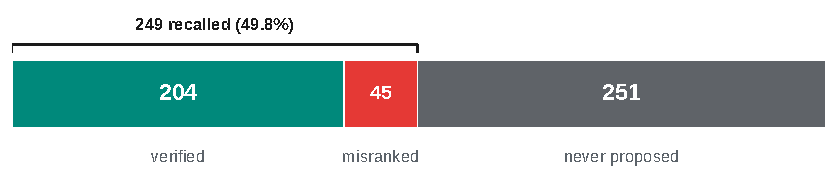
\includegraphics[width=0.92\linewidth]{fig_wall.pdf}
  \caption{Diagnostic wall: \textbf{locked $n{=}194$ instrumented slice}
  (58 verified / 7 mis-ranked / 129 never proposed).
  Expansion-106 has no forward-verify; this is \textbf{not} a pooled $n{=}300$ wall.
  Headline generation recall is 133/300.
  Never-proposed cases bind top-1 despite 89\% conditional precision (58/65).
  Same slice as Figure~\ref{fig:fig1}c.}
  \label{fig:fig-wall}
\end{figure}

\begin{table}[h]
\caption{Locked $n{=}194$ cases from released candidate files.
$^{13}$C chamfers in ppm; Tanimoto Morgan $r{=}2$. IDs are locked-round labels.}
\label{tab:cases}
\centering
\scriptsize
\setlength{\tabcolsep}{3.5pt}
\begin{tabular}{@{}lp{2.15cm}p{8.75cm}@{}}
\toprule
mode & id / formula & what failed \\
\midrule
\textbf{Proposal miss} &
main-R06 / C$_{29}$H$_{30}$FNO$_{2}$ &
True acridinedione never in the 3-candidate pool (Tanimoto-0.90 regioisomer: 4-fluorophenyl/phenyl swapped).
IR 1641, 1510~cm$^{-1}$; $^{13}$C 195.7. Verifier unused. \\
\textbf{Verify-save} &
v3-R25 / C$_{10}$H$_{14}$N$_{2}$O &
True 2-pyridyl picolinamide at self-rank 3; self-rank 1 is 3-pyridyl.
Forward-verify recovers (chamfer 0.42 vs 1.30~ppm). IR 1679~cm$^{-1}$.
Fig.~\ref{fig:fig-mechanism}. \\
\textbf{Verify-fail} &
v3-R26 / C$_{14}$H$_{11}$N$_{3}$O$_{3}$ &
True 3-nitrophenyl dihydroquinazolinone in pool (self-rank 2); 2-nitro ranked first.
Chamfer 1.35 vs 1.36~ppm. IR 1652, 1530, 1352~cm$^{-1}$. \\
\bottomrule
\end{tabular}
\end{table}

\begin{table}[h]
\caption{Expansion round (Claude Opus, InChIKey-14). Five $^{13}$C-overread flags stay in
the $n{=}300$ headline; validate-clean $n{=}295$ in Table~\ref{tab:clean295}.
Incomplete Fable arm (68/106) is never pooled.}
\label{tab:expansion}
\centering
\begin{tabular}{@{}lrr@{}}
\toprule
 & all ($n{=}106$) & clean ($n{=}101$) \\
\midrule
top-1 & 63/106 (59.4\%) & 61/101 (60.4\%) \\
generation recall & 68/106 (64.2\%) & 65/101 (64.4\%) \\
\bottomrule
\end{tabular}
\end{table}

\begin{table}[h]
\caption{Validate-clean sensitivity ($n{=}295$; five $^{13}$C-overread flags excluded).
Same scorer as Table~\ref{tab:headline}; not the headline.}
\label{tab:clean295}
\centering
\scriptsize
\setlength{\tabcolsep}{3pt}
\begin{tabular}{@{}lrrr@{}}
\toprule
metric & overall ($n{=}295$) & simple ($n{=}147$) & complex ($n{=}148$) \\
\midrule
top-1 exact constitution & 116/295 (39.3\%) [34--45] & 59.2\% [51--67] & 19.6\% [14--26] \\
recovered (top-3) & 130/295 (44.1\%) [39--49] & 63.9\% [56--71] & 24.3\% [17--31] \\
scaffold-level (best Tanimoto $\geq 0.45$) & 64\% & 80\% & 48\% \\
mean best Tanimoto & 0.66 & 0.79 & 0.53 \\
\bottomrule
\end{tabular}
\end{table}

By size on $n{=}295$: 67.9\% top-1 at $\leq$15 heavy atoms, 42.8\% at 16--25, 16.7\% above 25
($n{=}53/152/90$).
Full InChIKey (stereo): 93/295 (31.5\%) top-1 [26--37], recall 108/295 (36.6\%) [31--42].
Corpus-reweighted (17.5\% simple / 82.5\% complex): top-1 \textbf{26.5\%} [21--32], recall
\textbf{31.3\%} [25--37].
Self-ranking precision $|$ recall: 116/130 (89.2\%).

\end{document}
 shim for older compile notes.
% main_IRExpBench_only.tex is an optional orphan alternate --- not the ICLR build root.
% Headline n=300 generation (194 locked + all 106 expansion); fig_wall is the n=194 instrumented slice.
% expand-500: 230/230 deposited, unscored --- do not invent top-1 or a pooled wall.
% Compile with pdfLaTeX or XeLaTeX + BibTeX (references.bib + iclr2027_conference.bst).
% \iclrfinalcopy is the only official sty flag that prints \author and drops
% the left-margin submission ruler (see tex/iclr2027_conference.sty).
\documentclass{article}
\usepackage{iclr2027_conference,times}

\usepackage{hyperref}
\usepackage{url}
\usepackage{booktabs}
\usepackage{graphicx}
\usepackage{amsmath,amssymb}
\usepackage{enumitem}
\usepackage{placeins}
\usepackage{xcolor}
\usepackage{listings}
\usepackage{framed}
\lstdefinestyle{benchjson}{
  basicstyle=\ttfamily\scriptsize,
  breaklines=true,
  columns=fullflexible,
  keepspaces=true,
  showstringspaces=false,
  frame=none,
  literate={-}{-}1
}
\setlist{nosep,leftmargin=1.35em}
\setlength{\textfloatsep}{10pt plus 2pt minus 2pt}
\setlength{\floatsep}{8pt plus 2pt minus 2pt}
\setlength{\intextsep}{8pt plus 2pt minus 2pt}

\graphicspath{{figures/}{../figures/}{./}}

% Alternate Overleaf title (not used): Molecular Structure Elucidation with Frontier Models: A Benchmark on Literature-Reported IR, $^1$H, and $^{13}$C NMR Peak Lists
\title{Generation Recall, Not Verification, Binds LLM Structure Elucidation from Literature Spectra}

\author{
Ilkham Yabbarov\textsuperscript{1,$\dagger$},
Rudra Sondhi\textsuperscript{1},
Rodrigo A.\ Vargas-Hern\'andez\textsuperscript{1,2,3,$\dagger$}\\
\textsuperscript{1}Department of Chemistry and Chemical Biology, McMaster University,
Hamilton, Ontario L8S 4L8, Canada.\\
\textsuperscript{2}Brockhouse Institute for Materials Research, McMaster University,
Hamilton, Ontario L8S 4L8, Canada.\\
\textsuperscript{3}School of Computational Science and Engineering, McMaster University,
Hamilton, Ontario L8S 4L8, Canada.\\
$\dagger$\,\textit{E-mail:} yabbaroi@mcmaster.ca, vargashr@mcmaster.ca
}

\newcommand{\fix}{\marginpar{FIX}}
\newcommand{\new}{\marginpar{NEW}}

% Official ICLR 2027 switch: show \author and disable the submission linenumber
% ruler. The same flag also sets the running header to "Published as...".
% Double-blind (submit): keep \iclrfinalcopy commented; \maketitle then prints
% "Anonymous authors / Paper under double-blind review". Camera-ready: uncomment
% \iclrfinalcopy and delete the \lhead override below.
% \iclrfinalcopy  % OFF for double-blind submission; re-enable for camera-ready
\begin{document}

\maketitle
\lhead{Under review as a conference paper at ICLR 2027}

\begin{abstract}
Frontier large language models are often cast as near-solved structure elucidators on
curated spectra. We ask the operational question: given only the molecular formula and
\textbf{literature-reported} IR / $^1$H / $^{13}$C \textbf{peak lists} --- not digitised
traces --- can an off-the-shelf LLM recover constitution, and \textbf{which stage fails}
when it cannot?

The binding claim is \textbf{propose $\gg$ verify}: candidate proposal, not ranking,
is the expensive stage.
We release \textbf{IRSpectra-Bench}, a blind peak-list benchmark of \textbf{300}
compounds (194 locked $+$ all 106 Opus expansion, flags included) drawn from the
companion \textbf{IRexp} band-list resource~\citep{yabbarov2026irexp} --- cited
here, not re-described --- with a fixed RDKit InChIKey-connectivity contract and
decomposable \textbf{generation recall} / \textbf{verification precision} metrics.
A frontier LLM recovers \textbf{39\%} top-1 (118/300; 95\% CI 34--45), or
\textbf{27\%} after corpus reweighting; generation recall is \textbf{44\%} (133/300).
On the forward-verified $n{=}194$ slice the true structure enters the pool for only
\textbf{34\%} of compounds, yet training-free forward-verification selects it
\textbf{89\%} of the time once proposed (58/65).
The expansion slice is easier (59\% vs 28\% top-1) and is disclosed, not hidden.
A larger deposited blind round toward $n{\approx}500$ is \textbf{unscored} and is
not in this headline.
The same recall $\ll$ precision asymmetry replicates across \textbf{four vendor families}.
Formula-only controls collapse; accuracy is flat in source-paper year; generate-wide
sampling lifts recall where verification alone barely moves top-1.
Recovered from published top-$k$ figures, recall carries \textbf{68--83\%} of the accuracy
collapse from curated or simulated spectra to real heterogeneous peak lists.
Frozen predictions, scorers and code are released for mechanical re-evaluation.
\end{abstract}

\section{Introduction}
\label{sec:introduction}

Structure elucidation from spectra sits at the centre of synthetic and analytical chemistry,
and machine learning increasingly treats it as a sequence or agent task.
Encoder--decoder models train on paired corpora~\citep{chacko2024spectro,ottomano2025nmiracle,alberts2024ir};
LLM agents and puzzle benches report high recovery on curated or education
spectra~\citep{kamber2026chemist,guo2024molpuzzle,zhuang2025treesearch,espejo2026agentic}.
Cross-paper numbers swing wildly with harness (e.g.\ GPT-4o from 1.4\% to 57.8\% on MolPuzzle
under different prompting~\citep{guo2024molpuzzle,zhuang2025treesearch}).
What remains under-measured is the harder operational task: \textbf{taking peak lists as
printed in open-access papers and recovering constitution} with an off-the-shelf model,
a fixed molecular-representation scoring contract, and an honest account of
\textbf{which stage of elucidation binds} --- proposal versus verification.

We argue that end-to-end top-1 alone is the wrong reporting primitive.
Any system that returns a ranked candidate list factorises as
\begin{equation}
\text{top-1} \;=\; \underbrace{P(\text{true} \in \text{pool})}_{\text{generation recall}}
\times
\underbrace{P(\text{rank}=1 \mid \text{true} \in \text{pool})}_{\text{verification precision}}.
\end{equation}
These rates have different denominators and must not be differenced.
Prior work already notes that re-ranking cannot recover a missing
candidate~\citep{priessner2026reasoning}; we supply the missing \textbf{measurement
infrastructure at scale}.

\paragraph{Contributions.}
\begin{enumerate}
  \item \textbf{IRSpectra-Bench} --- a blind, complexity-stratified peak-list benchmark ($n{=}300$)
        with a pre-registered InChIKey-connectivity scorer and community reporting contract
        (top-1, generation recall, verification precision $|$ recall).
  \item \textbf{A recall-bound diagnosis} on a frontier LLM: propose $\gg$ verify.
        Generation recall is 44\% on the pooled $n{=}300$ cohort; on the $n{=}194$
        instrumented slice, 34\% proposed and 89\% selected once proposed; that slice's
        top-1 moves only 28\% $\to$ 30\% under training-free forward-verification.
  \item \textbf{Contamination and cross-vendor controls} --- formula-only and recency bounds;
        four-vendor replication of recall $\ll$ precision.
  \item \textbf{A literature decomposition} that recovers the same split from published top-$k$
        figures, showing recall carries most of the collapse on real heterogeneous data.
\end{enumerate}

\paragraph{Dataset pointer (resource, not co-headline).}
Band lists come from the companion \textbf{IRexp} resource (121,233 records; 43,060
structure-linked; 33,201 full IR+$^1$H+$^{13}$C+structure quadruples); an anonymised
review copy is in Appendix~\ref{app:dataset}.
Construction and licensing live in a \textit{Scientific Data} manuscript (in
preparation)~\citep{yabbarov2026irexp}.
This ICLR paper \textbf{cites} that resource and does not re-present a Data Descriptor.

\begin{figure}[t]
  \centering
  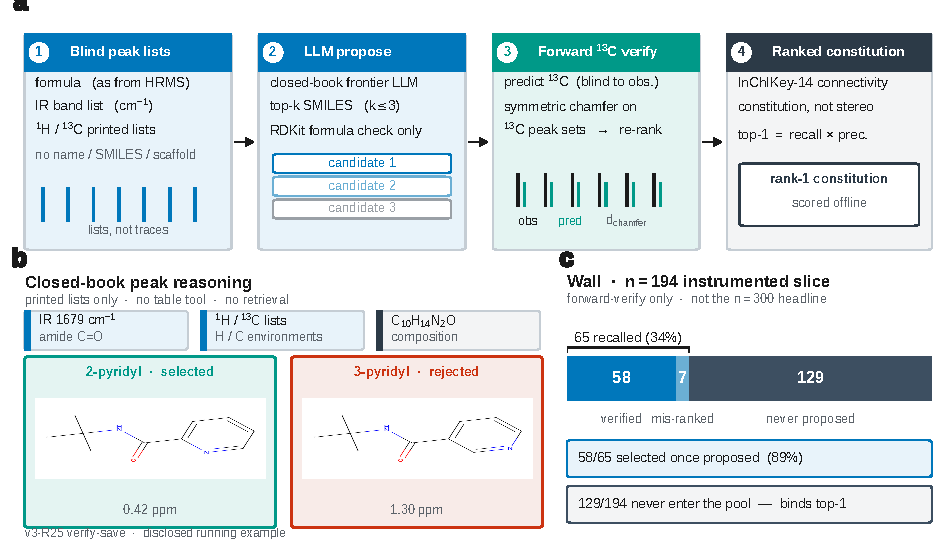
\includegraphics[width=\linewidth]{fig1_overview.pdf}
  \caption{IRSpectra-Bench protocol.
  (a)~Printed IR/$^1$H/$^{13}$C lists $+$ formula $\rightarrow$ closed-book LLM
  proposes top-$k$ SMILES (RDKit formula check) $\rightarrow$ forward $^{13}$C
  (blind) $\rightarrow$ chamfer re-rank $\rightarrow$ InChIKey-14.
  (b)~Evidence is the lists themselves (no peak-table tool, no retrieval).
  Running example v3-R25 (IR 1679~cm$^{-1}$; chamfer 0.42 vs 1.30~ppm).
  (c)~Locked $n{=}194$ instrumented wall: 58 verified / 7 mis-ranked / 129 never
  proposed. \textbf{Not} a pooled $n{=}300$ wall
  (headline generation: Table~\ref{tab:headline}; diagnostic repeat:
  Figure~\ref{fig:fig-wall}).}
  \label{fig:fig1}
\end{figure}

\section{Related work}
\label{sec:related-work}

\paragraph{Trained spectra $\to$ structure models.}
Sequence and graph decoders on paired
corpora~\citep{chacko2024spectro,hu2024multitask,yang2026nmrtrans,ottomano2025nmiracle,alberts2024ir,alberts2025benchmarks}
are accurate in-distribution but typically scored end-to-end.
We do not claim to beat them on IRSpectra-Bench; Spectro, NMIRacle, Alberts IR transformers
and CASE are \textbf{not yet scored} on our bench (Section~\ref{sec:limitations}) --- a gap we
state honestly and leave to the released scorer.

\paragraph{Agentic elucidation: three regimes.}
The contrast is the \textbf{setting and the stage split}, not a method scoreboard.
(i)~\emph{Tool-using lab agents} --- ChemCrow~\citep{mbran2024chemcrow},
Coscientist~\citep{boiko2023coscientist} --- show that LLMs can call instruments and
planners; they do not measure which elucidation stage binds.
(ii)~\emph{Spectrum-native agents} improve \emph{how} a model reads a spectrum or
re-ranks a \textbf{fixed} pool: tree-search~\citep{zhuang2025treesearch},
SpecMol~\citep{shen2025specmol}, Priessner \textit{et al.}~\citep{priessner2026reasoning},
NMR-Solver~\citep{jin2025nmrsolver}, NMRAgent~\citep{fang2026nmragent}.
Priessner already notes that re-ranking cannot recover a missing candidate; we measure
that failure at literature-peak-list scale.
SpectraLLM~\citep{su2025spectrallm} is a \textbf{fine-tuned} multi-spectral elucidator
on \textbf{simulated} corpora (QM9S DFT; Alberts USPTO multimodal) --- a different object
and a different training regime; we do not score it here.
IR-Agent~\citep{noh2025iragent} (ICLR 2026) is the closest concurrent multi-agent IR
elucidator: on \textbf{NIST experimental IR} a translator proposes a SMILES pool, TI+Ret
enrich local (peak-table) and global (retrieved-spectrum) features, and an SE expert
re-ranks (Top-$k$ SMILES; atom type / scaffold / carbon count may be prompt-injected).
(iii)~\emph{Agentic-search benches} --- MolQuest~\citep{han2026molquest},
NMRGym~\citep{fang2026nmrgym}, Espejo Morales \textit{et al.}~\citep{espejo2026agentic}
(education $\to$ industrial instrument files: 80.9\% $\to$ 20.6\%) --- ask which
architecture or abductive loop wins.
IRSpectra-Bench is the harder operational object: \textbf{literature peak lists}
(IR+$^1$H/$^{13}$C+formula as from HRMS), \textbf{off-the-shelf} closed-book models, no
name, SMILES, or scaffold hint.
We measure \textbf{which stage binds} after spectra are read --- generation recall versus
verification precision $|$ recall --- on pooled $n{=}300$, with instrumented
forward-verify on $n{=}194$.
IR-Agent's SE expert over a \textbf{fixed candidate pool} is exactly the regime our
ladder diagnoses as recall-limited (proposal binds; conditional forward-verify
$\approx$89\%, 58/65).
TI+Ret can enrich \emph{features} but does \textbf{not} remove a proposal wall if the true
structure never enters the pool.
Architecture search that does not change $P(\text{true}\in\text{pool})$ cannot move
top-1 on a recall-bound bench.
We do not claim to beat SpectraLLM or IR-Agent on their native sets; neither is scored
here.
\begin{center}
\scriptsize
\setlength{\tabcolsep}{4pt}
\begin{tabular}{@{}llll@{}}
\toprule
 & input & metric & binds \\
\midrule
IR-Agent & NIST experimental IR & Top-$k$ SMILES & re-rank given pool \\
this paper & lit.\ IR+$^1$H/$^{13}$C+formula lists & recall vs prec.$|$recall & proposal \\
\bottomrule
\end{tabular}
\end{center}

\paragraph{Heterogeneous data, CASE, and positioning.}
Most prior suites use simulated or single-instrument spectra; we use literature-reported
peak lists across thousands of laboratories and report formula-only and recency controls
(Section~\ref{sec:contamination}).
Matching predicted to observed shifts --- DP4~\citep{smith2010dp4},
CASE~\citep{elyashberg2012case}, NMR-Solver, NMRAgent --- is easier than inverse
generation; CASE enumerators have exhaustive recall by construction, while the LLM
literature almost never reports whether the true structure was proposed at all.
SpecX~\citep{xiang2026specx} bounds a related multi-modal spectroscopy task on
simulated traces.
IRSpectra-Bench is an openly redistributable literature-peak-list suite with a
\textbf{stage decomposition}, measured on Claude and replicated across three other
model families.

\FloatBarrier
\section{IRSpectra-Bench}
\label{sec:benchmark}

\subsection{Task and inputs}

Each of 300 problems supplies the \textbf{molecular formula} (as from HRMS), the \textbf{IR
band list} (cm$^{-1}$), and \textbf{$^1$H / $^{13}$C shift lists} --- exactly the textual form
reported in open-access papers.
No name, SMILES or scaffold hint.
Inputs are author-transcribed \textbf{band and shift lists}, not absorbance traces or FIDs:
a different object from digitised-spectrum benchmarks~\citep{espejo2026agentic}, and one that
matches how language models consume literature.

The cohort is the pre-registered pool of a locked 194 (spectrally validated main round 134 $+$
60 controls) and a 106-compound expansion draw ($n{=}300{=}194{+}106$).
Five expansion records fail the same $^{13}$C-overread audit used on the main round and are
included in the 300 (validate-clean $n{=}295$ in Appendix~\ref{app:extended}).
Problems are drawn from the structure-complete split of IRexp (\texttt{irexp\_resolved}; see
companion Data Descriptor)~\citep{yabbarov2026irexp}.
On the locked 194, author peak assignments name a ring system in 10/194; those are solved
1/10 vs 54/184 for the rest, so named-ring annotation does not drive that slice.
Figure~\ref{fig:fig-chemspace} summarises the chemistry space of the pooled headline.
Figure~\ref{lst:payload} is the solver-facing contract: formula plus printed peak lists,
gold constitution held out.

\begin{figure}[ht]
  \centering
  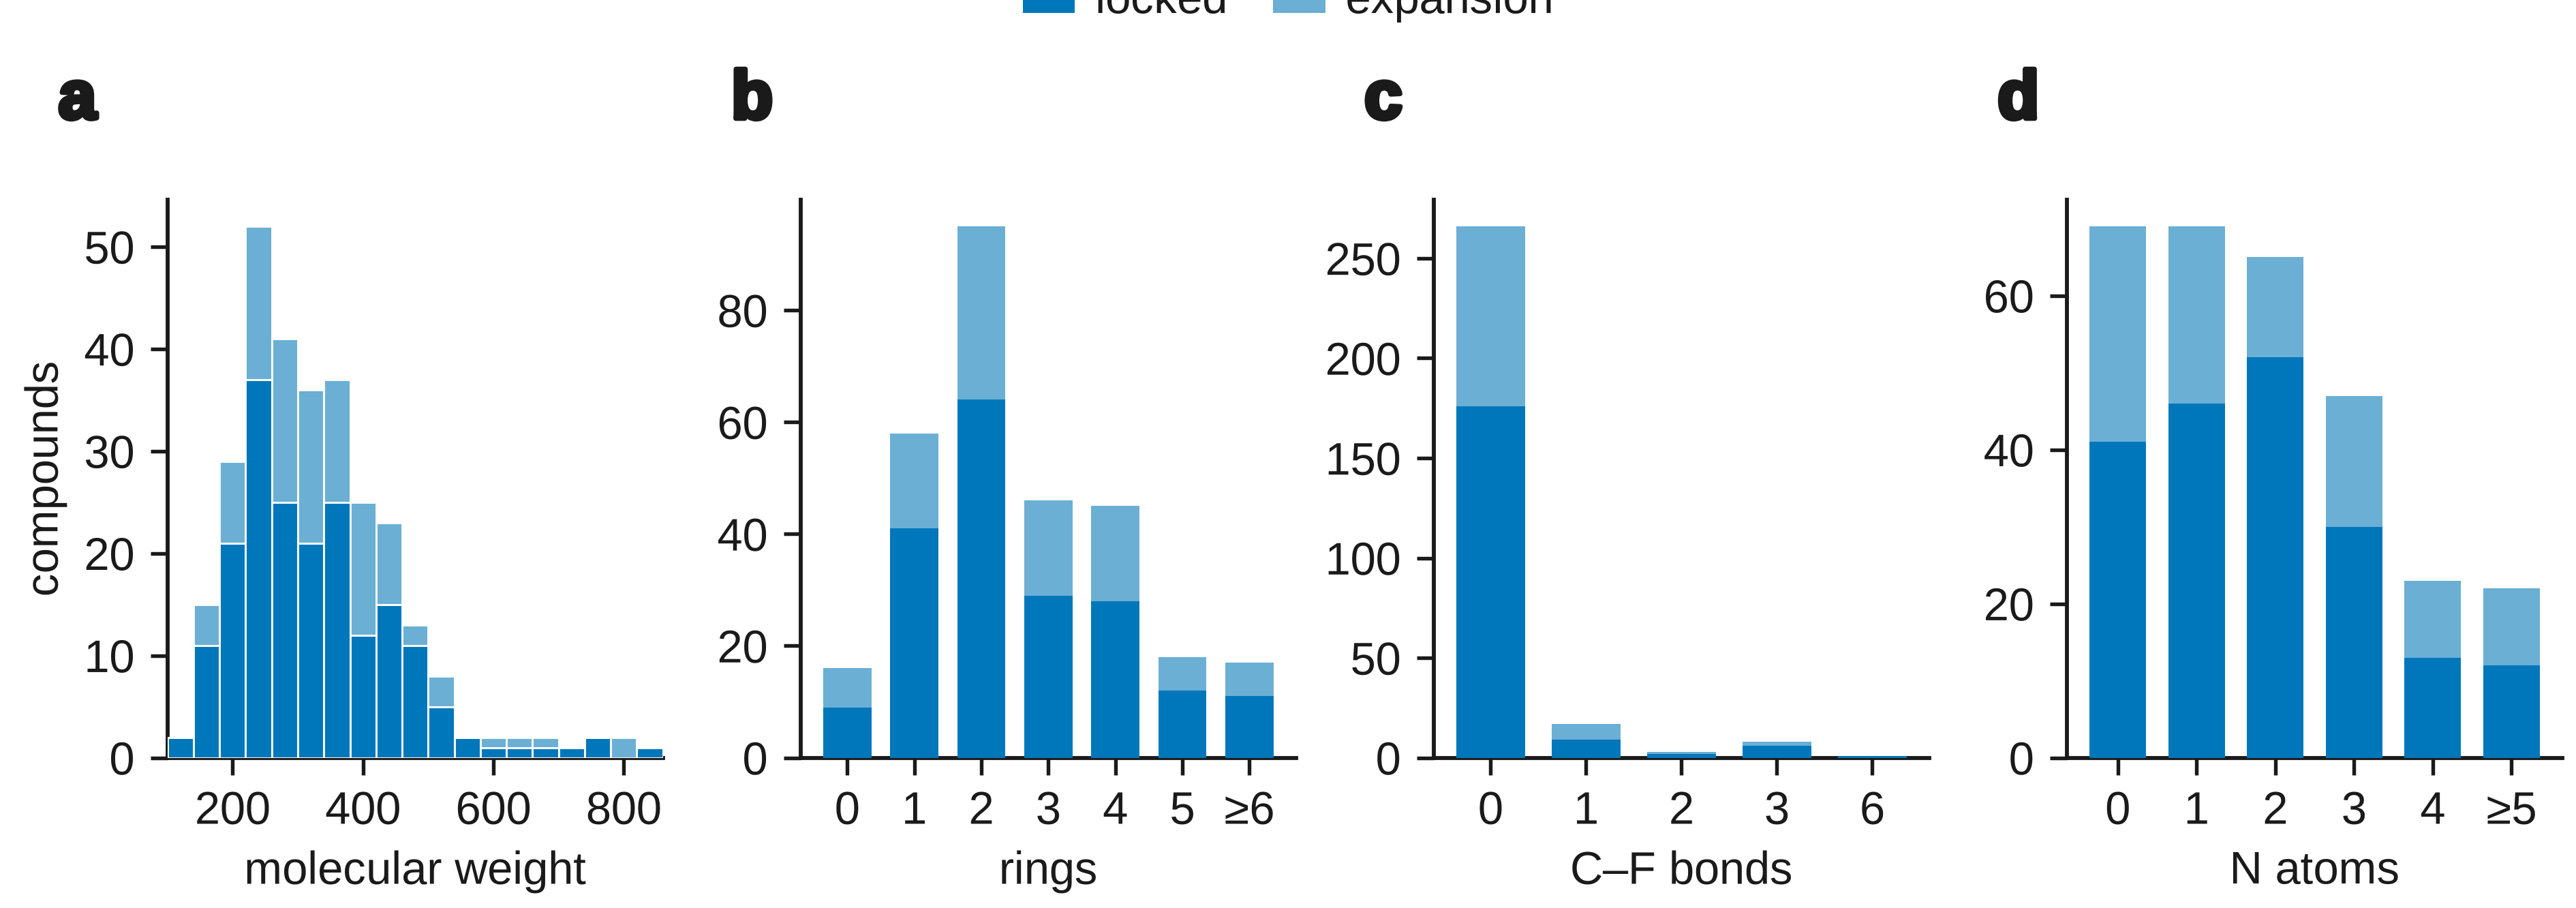
\includegraphics[width=0.92\linewidth]{fig_chemspace.png}
  \caption{Pooled headline chemistry ($n{=}300$; panels on validate-clean $n{=}295$).
  (a)~MW (median 306). (b)~RDKit rings (median 2). (c)~C--F bonds. (d)~N atoms.
  Stacked: locked (dark) vs expansion (light). Mid-size literature space, not a NIST toy set.}
  \label{fig:fig-chemspace}
\end{figure}

\subsection{Difficulty, balance, and scoring contract}

\textbf{Difficulty} is declared \emph{a priori} by RDKit ring analysis: \emph{simple} iff
$\leq$2 rings, no fused/spiro/bridgehead system, $\leq$22 heavy atoms; else \emph{complex}
(151/149 on $n{=}300$).
The released benchmark is \textbf{50/50 by design}; the eligible corpus is 17.5\% simple /
82.5\% complex.
Reweighted to corpus composition on the validate-clean subset, top-1 falls 39.3\% $\to$
\textbf{26.5\%} [21--32] and recall 44.1\% $\to$ \textbf{31.3\%} [25--37]
(Appendix~\ref{app:extended}).
We report both: the reweighted figure is the better estimate for an arbitrary paper, and the
50/50 figure is the comparable leaderboard number (Table~\ref{tab:headline}).

\textbf{Scoring.} A prediction is correct if RDKit InChIKey \textbf{connectivity} (first 14
characters) matches --- we score \emph{constitution}.
Full stereo-sensitive InChIKey is reported on the validate-clean subset
(Appendix~\ref{app:extended}).
External submissions: up to three ranked SMILES per \texttt{qid}, no structure hints
(\texttt{docs/LEADERBOARD.md}; \texttt{scripts/score\_submission.py}).
Primary metrics (report all three): \textbf{top-1} (best-ranked candidate matches at
connectivity); \textbf{generation recall} (reference in the pool \emph{before} re-ranking);
\textbf{verification precision $|$ recall} (correct top-1 among recall-positive compounds).
Confidence intervals are bootstrap 95\%; paired model differences use McNemar with Holm correction.

\section{Experimental setup}
\label{sec:setup}

\paragraph{Blind payload and solver.}
The solver sees four JSON fields per \texttt{qid}: \texttt{formula} (as from HRMS),
\texttt{ir\_bands\_cm-1}, \texttt{h\_nmr}, \texttt{c\_nmr} --- peak lists as printed
(Figure~\ref{lst:payload}).
No name, SMILES, scaffold, atom-type hint, or retrieved spectrum; ground truth is scored
offline.
Frontier LLM agent (Claude Opus via consumer subscription), closed-book, one sub-agent per
batch, RDKit formula check only.
No fine-tuning, no paid API, \textbf{no thinking tier} for the core protocol.
Inference is \textbf{not} exactly reproducible (no pinned snapshot, temperature or seed ---
Section~\ref{sec:limitations}).
\textbf{Scoring is reproducible}: frozen predictions, ground truth and scorers regenerate every
training-free number.

\begin{figure}[ht]
\centering
\begin{minipage}{0.98\linewidth}
\begin{framed}
\noindent
\begin{minipage}[c]{0.56\linewidth}
\begin{lstlisting}[style=benchjson]
{
  "qid": "v3-R25",
  "formula": "C10H14N2O",
  "ir_bands_cm-1": [1679, "..."],
  "h_nmr": "[printed 1H list]",
  "c_nmr": "[printed 13C list]"
}
\end{lstlisting}
\end{minipage}\hfill
\begin{minipage}[c]{0.40\linewidth}
\centering
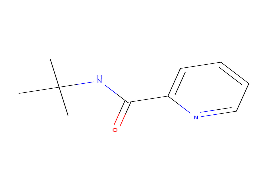
\includegraphics[width=\linewidth]{fig_listing_mol.pdf}\\[0.2em]
{\scriptsize\itshape gold held out}\\[-0.1em]
{\scriptsize 2-pyridyl picolinamide}
\end{minipage}
\end{framed}
\end{minipage}
\caption{\textbf{Listing 1.} Solver-facing payload (abridged), IRexp
JSON$+$molecule layout. Gold constitution (right) is held out.
Only disclosed fragments are shown (v3-R25 / C$_{10}$H$_{14}$N$_{2}$O / IR 1679);
full lists ship with the bench. Source: IRexp~\citep{yabbarov2026irexp};
this PDF is not a Data Descriptor.}
\label{lst:payload}
\end{figure}

\paragraph{Scoring contract and candidate budget.}
A deposit is JSONL of \texttt{\{qid, candidates: [SMILES,\ldots]\}} under a stated budget.
The scorer reports the three Section~\ref{sec:benchmark} metrics at InChIKey-connectivity,
with bootstrap 95\% CIs.
Self-ranking vs forward-verified re-ranking must be labelled; they are not interchangeable.
Headline protocol: $\leq$3 ranked SMILES per \texttt{qid}.
On the 60-compound arm Claude returned mean 2.20 candidates vs 3.00 for the other vendors
(recall rankings approximate).
\textbf{Generate-wide} (that arm only): ten independent solvers $\times$ up to six SMILES,
pooled then re-ranked --- not the $n{=}300$ reporting budget.

\paragraph{Forward-verification, expansion, and probes.}
Generate $\to$ forward-predict $^{13}$C (blind to the observed list) $\to$ re-rank by
symmetric chamfer on $^{13}$C peak sets (Section~\ref{sec:forward-verify}); instrumented on
the locked $n{=}194$ only.
Expansion is a pre-registered 106-compound draw from the same \texttt{irexp\_resolved}
sampler after the $n{=}194$ lock, with the same $^{13}$C-overread audit
(Section~\ref{sec:expansion}): five flags stay in the $n{=}300$ headline; validate-clean
$n{=}295$ is appendix; expansion-106 forward-verify was not run.
A later 230-compound draw toward $n{\approx}500$ is deposited and unscored
(Section~\ref{sec:expansion}).
Controls: formula-only / recency (Section~\ref{sec:contamination}); four-vendor replication
on a 60-compound arm (Section~\ref{sec:cross-vendor}); generate-wide sampling; HOSE lookup
and GNN $^{13}$C verifiers; small IRexp-fine-tuned generator probe (excluded from headline
claims).

\section{Results}
\label{sec:results}

\subsection{Headline performance}
\label{sec:headline}

\begin{table}[ht]
\caption{Headline elucidation ($n{=}300{=}194$ locked $+$ $106$ expansion).
Bootstrap 95\% CIs; validate-clean $n{=}295$ in Appendix~\ref{app:extended}.}
\label{tab:headline}
\centering
\small
\begin{tabular}{@{}lr@{}}
\toprule
metric & $n{=}300$ \\
\midrule
top-1 exact constitution & \textbf{39.3\%} (118/300) [34--45] \\
\quad simple ($n{=}151$) & 58.3\% (88/151) \\
\quad complex ($n{=}149$) & 20.1\% (30/149) \\
generation recall (top-3) & \textbf{44.3\%} (133/300) [39--50] \\
\bottomrule
\end{tabular}
\end{table}

On the validate-clean subset, scaffold-level recovery is 64\% (simple 80\%, complex 48\%) and
mean best Tanimoto is 0.66; accuracy falls with size (67.9\% top-1 at $\leq$15 heavy atoms,
42.8\% at 16--25, 16.7\% above 25; $n{=}53/152/90$; Appendix~\ref{app:extended}).
On the locked 194, of 137 analysable top-1 misses, \textbf{76.6\%} are constitutional isomers of the true
structure; only \textbf{22.6\%} share the true Murcko scaffold --- wrong connectivity at the
right composition, not mostly fine regiochemistry (not re-run on the expansion).
A 24-compound four-model Claude comparison is capability-sensitive (Haiku $\subset$ Sonnet
$\subset$ Opus $\subset$ Fable) but underpowered for adjacent ranks, with a disclosed protocol
asymmetry (Section~\ref{sec:limitations}); a battery-electrolyte subset ($n{=}46$) matches the
locked-slice regime (26\% top-1; recall-bound).

\begin{table}[ht]
\caption{Generation by slice. Headline is pooled $n{=}300$, not locked 194 alone.}
\label{tab:slices}
\centering
\small
\begin{tabular}{@{}lrrr@{}}
\toprule
 & locked ($n{=}194$) & expansion ($n{=}106$) & pooled ($n{=}300$) \\
\midrule
top-1 & 55/194 (28.4\%) & 63/106 (59.4\%) & \textbf{118/300 (39.3\%)} \\
generation recall & 65/194 (33.5\%) & 68/106 (64.2\%) & \textbf{133/300 (44.3\%)} \\
\bottomrule
\end{tabular}
\end{table}

The expansion slice is easier for this solver than the locked 194 (59.4\% vs 28.4\% top-1);
pooling does not hide that gap.
Self-ranking precision $|$ recall on the pooled generation cohort is 118/133 (88.7\%) ---
that is \emph{not} forward-verification precision (Section~\ref{sec:forward-verify}).

\subsection{Is the model reading the spectra?}
\label{sec:contamination}

\begin{table}[ht]
\caption{Formula-only control (paired, $n{=}60$).}
\label{tab:formula-only}
\centering
\small
\begin{tabular}{@{}lrr@{}}
\toprule
condition & top-1 & recovered (top-3) \\
\midrule
formula only & \textbf{3/60 (5\%)} & 3/60 (5\%) \\
formula + IR + $^1$H + $^{13}$C & 14/60 (23\%) & 19/60 (32\%) \\
\bottomrule
\end{tabular}
\end{table}

Outcomes are perfectly nested (McNemar $p{=}0.001$).
Accuracy is flat in source-paper year across the locked 194 ($r{=}{-}0.007$), bounding pretraining
recall of specific papers.
We claim a \textbf{strong bound, not exclusion} of contamination
(Section~\ref{sec:limitations}).

\begin{figure}[ht]
  \centering
  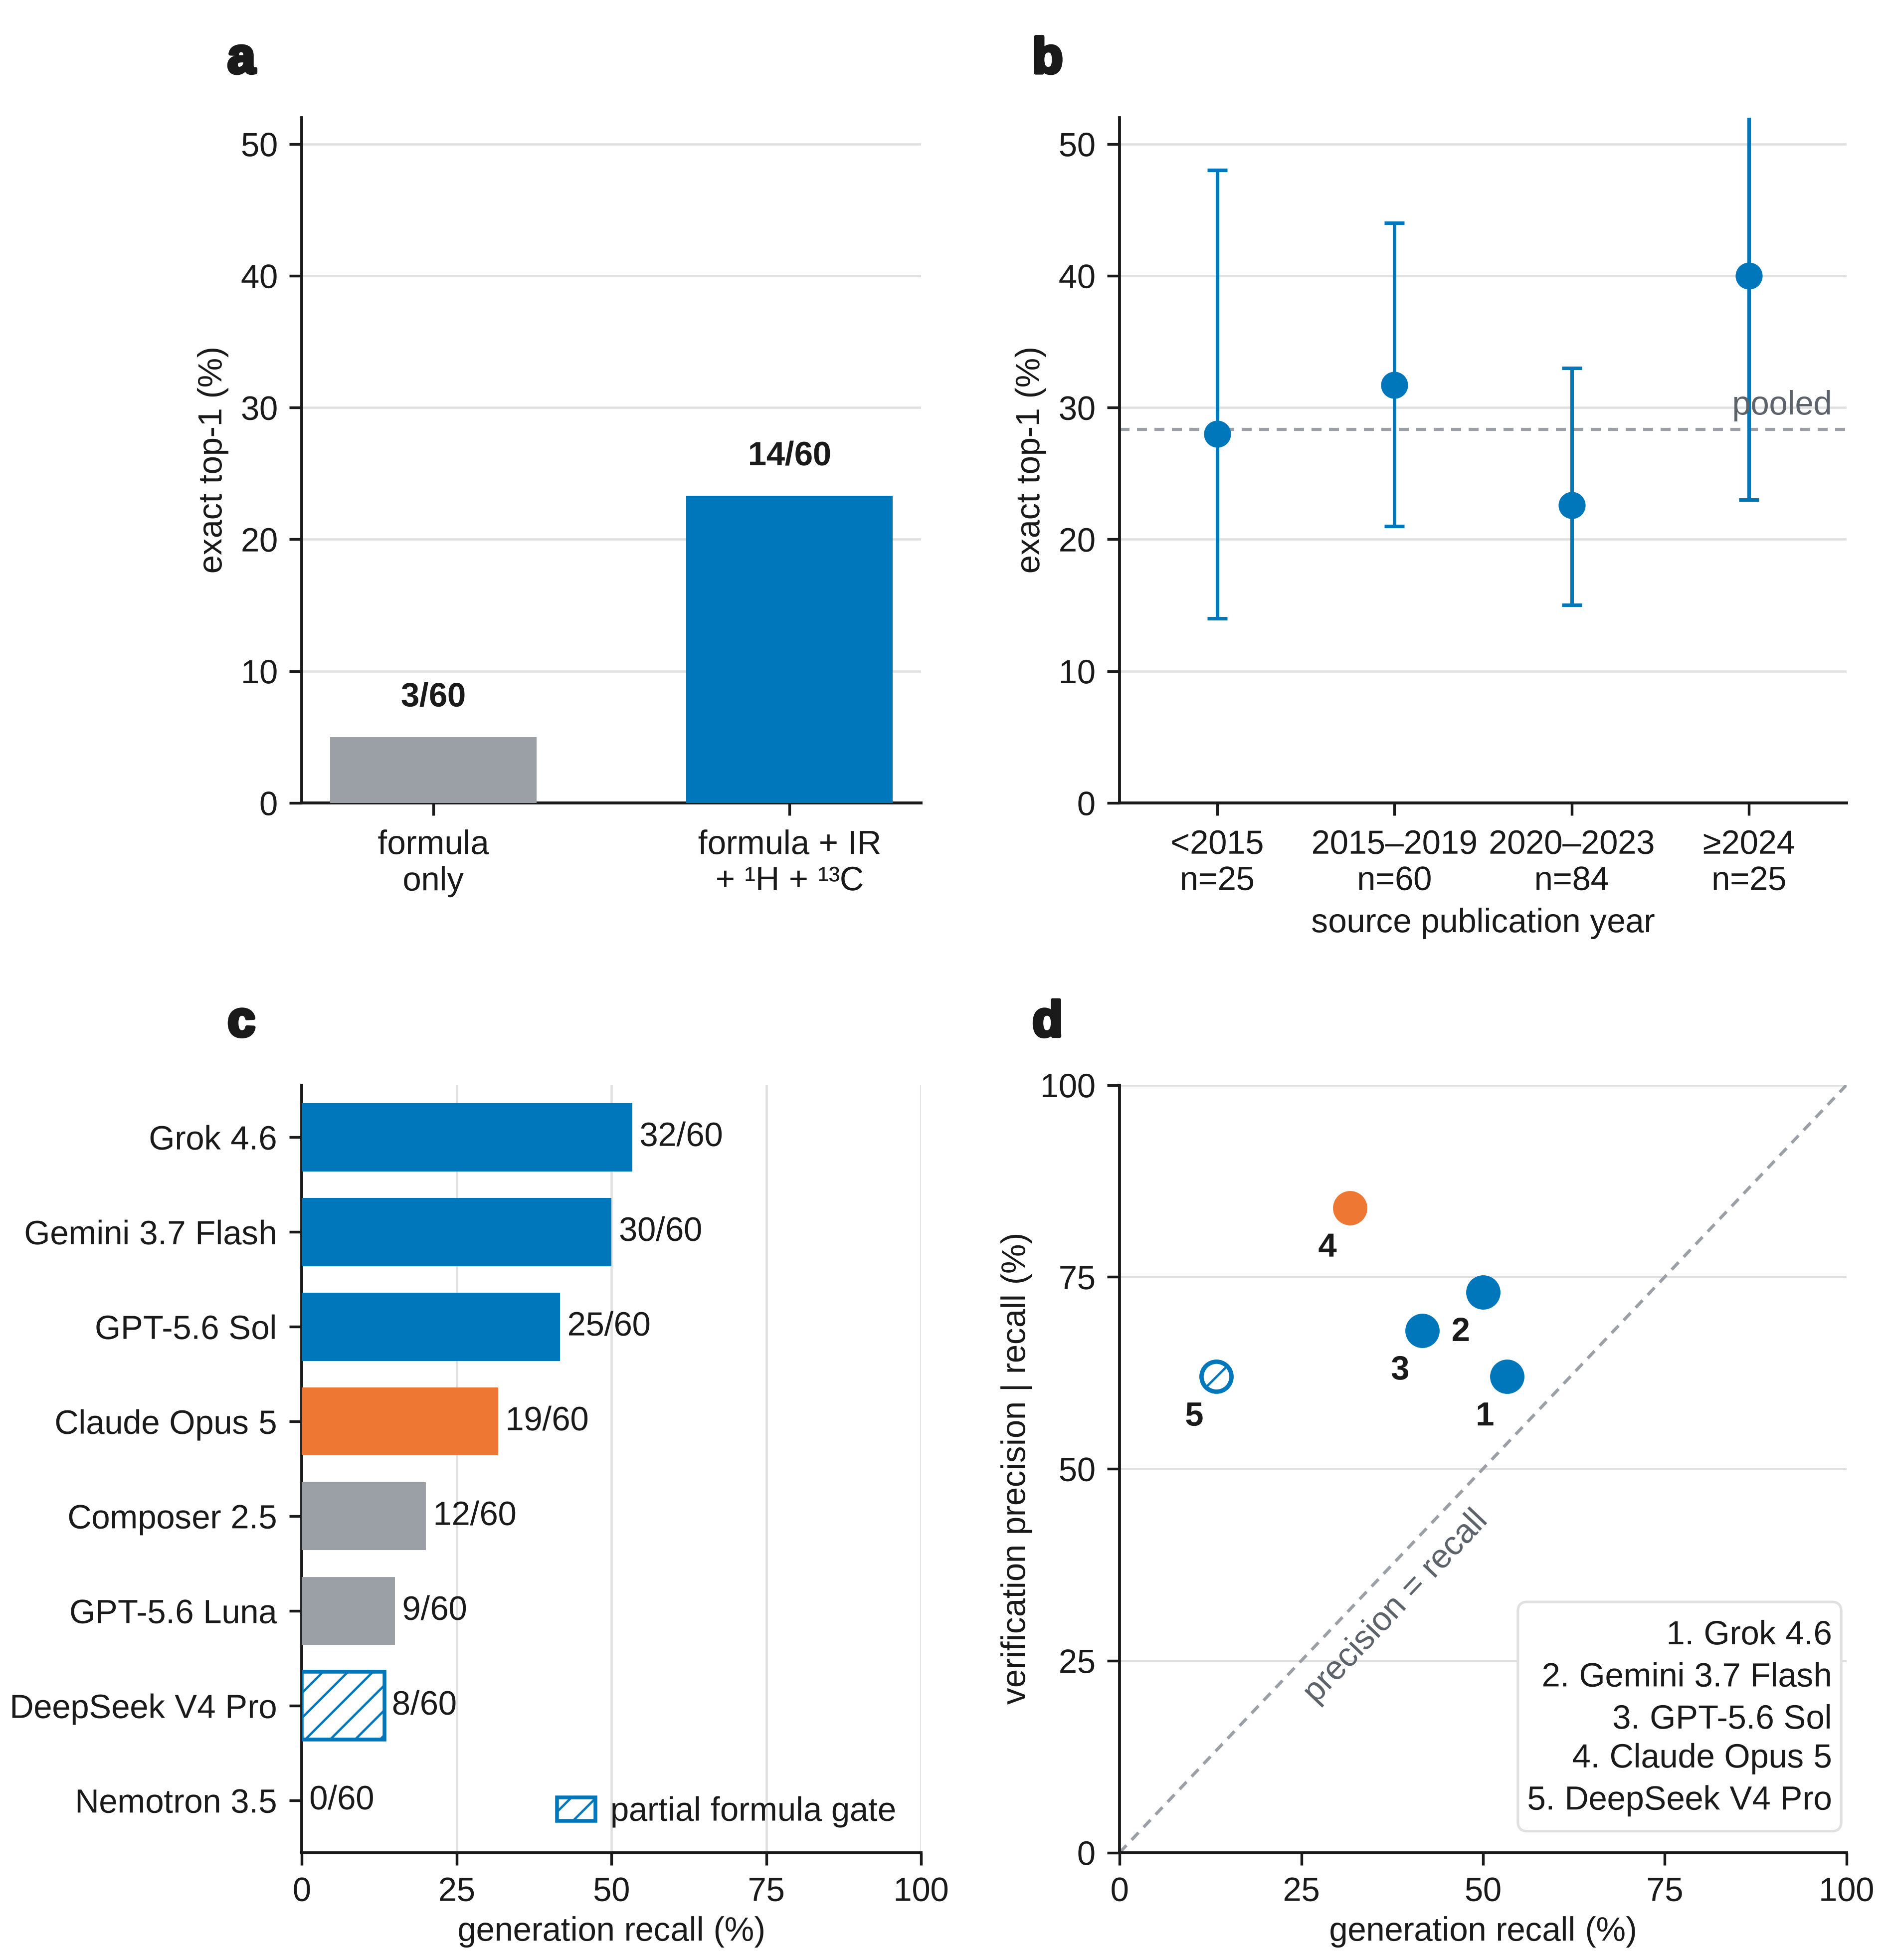
\includegraphics[width=0.62\linewidth]{fig_robustness.png}
  \caption{Robustness on instrumented arms (formula-only / cross-vendor $n{=}60$;
  recency $n{=}194$): formula-only collapse, flat recency, four-vendor recall $\ll$ precision.}
  \label{fig:fig-robustness}
\end{figure}

\subsection{Cross-vendor replication}
\label{sec:cross-vendor}

Grok 4.6, Gemini 3.7 Flash and GPT-5.6 Sol solved the same 60-compound arm under the
identical protocol.
\textbf{Verification precision exceeds generation recall in every arm}; bootstrapping
separates the paired gap for Claude (+52.5 points), GPT-5.6 Sol (+26.3) and Gemini (+23.3);
Grok's gap (+9.2) is directional.

\begin{table}[ht]
\caption{Cross-vendor decomposition ($n{=}60$). Recall and precision use different denominators.}
\label{tab:cross-vendor}
\centering
\small
\begin{tabular}{@{}lrrr@{}}
\toprule
model & generation recall & verification precision $|$ recall & multi-candidate only \\
\midrule
Claude Opus & 19/60 = 32\% & 16/19 = 84\% & 10/13 = 77\% \\
Grok 4.6 & 32/60 = 53\% & 20/32 = 62\% & 20/32 = 62\% \\
Gemini 3.7 Flash & 30/60 = 50\% & 22/30 = 73\% & 22/30 = 73\% \\
GPT-5.6 Sol & 25/60 = 42\% & 17/25 = 68\% & 16/24 = 67\% \\
\bottomrule
\end{tabular}
\end{table}

Candidate budgets differ (Claude mean 2.20 vs others 3.00), so recall rankings are
approximate.
A clean-clone control for Grok bounds key leakage (McNemar $p{=}0.39$).

\subsection{Forward-verification decomposition}
\label{sec:forward-verify}

\begin{figure}[ht]
  \centering
  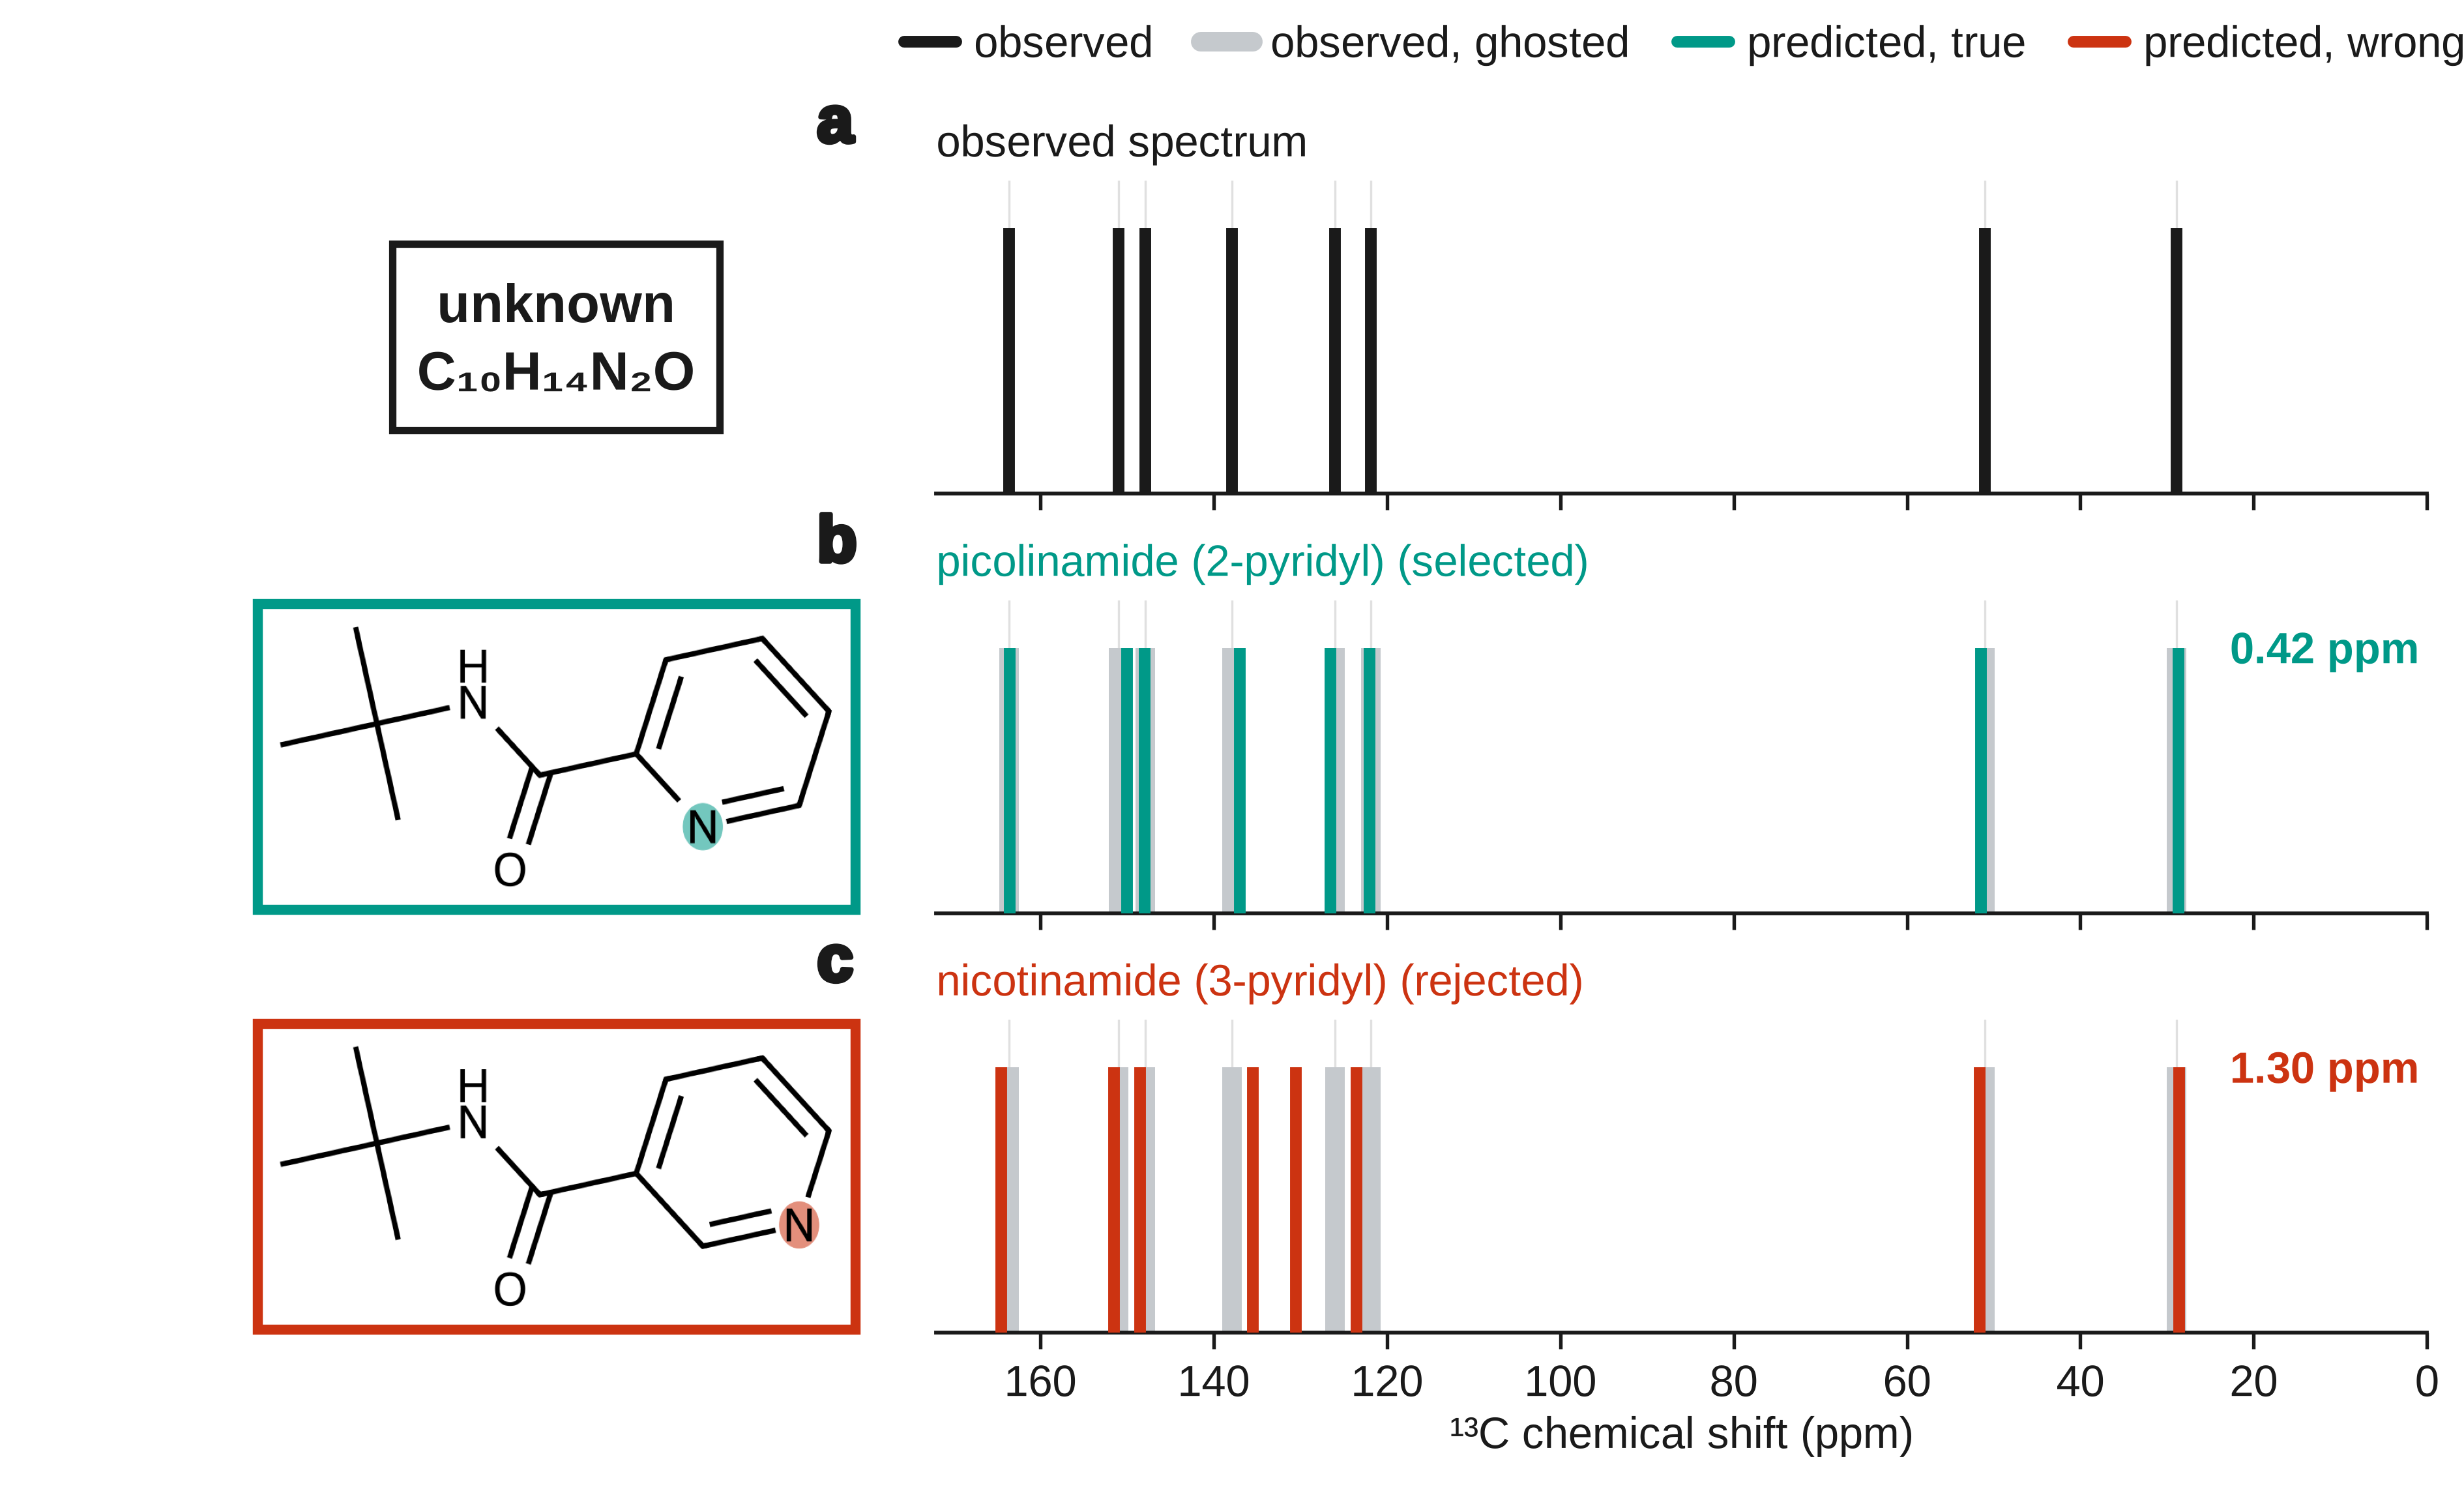
\includegraphics[width=0.72\linewidth]{fig_mechanism.png}
  \caption{Locked v3-R25: self-rank prefers 3-pyridyl; forward $^{13}$C recovers 2-pyridyl
  (chamfer 0.42 vs 1.30~ppm) --- a verify-save, not a recall win (Table~\ref{tab:cases}).}
  \label{fig:fig-mechanism}
\end{figure}

\begin{table}[ht]
\caption{Forward-verify on the instrumented slice ($n{=}194$).
Pooled $n{=}300$ in Table~\ref{tab:headline} is generation only.}
\label{tab:fverify}
\centering
\small
\begin{tabular}{@{}lrr@{}}
\toprule
 & 60-compound arm & locked slice ($n{=}194$) \\
\midrule
generation recall & 19/60 (32\%) & 65/194 (34\%) \\
top-1, solver self-ranking & 14/60 (23\%) & 55/194 (28\%) \\
top-1, forward-verified re-ranking & 16/60 (27\%) & 58/194 (30\%) \\
precision $|$ recall --- forward-verification & 16/19 (84\%) & 58/65 (\textbf{89\%}) \\
multi-candidate only --- forward-verification & 10/13 (77\%) & 30/37 (81\%) \\
\bottomrule
\end{tabular}
\end{table}

When the true structure is among the candidates, forward-verification selects it in 58/65
cases (89\%).
Where a choice existed ($n{=}37$), forward-verification is correct on 30/37 (81\%) against a
54.0\% derangement floor (+27.1 points).
The margin over self-ranking is \textbf{small and unresolved} (seven gained, four lost;
McNemar $p{=}0.55$) --- we do \textbf{not} claim an accuracy advance.
Precision is high while recall binds: no re-ranking repairs the 129/194 compounds on this
slice where the true structure was never proposed (Figure~\ref{fig:fig1}c;
diagnostic repeat in Figure~\ref{fig:fig-wall}).

\paragraph{Worked cases.}
Three locked-slice deposits instantiate the wall (Appendix Table~\ref{tab:cases}; expansion
qids reuse R22/R25 --- IDs below are locked-round labels).
\textbf{main-R06} (C$_{29}$H$_{30}$FNO$_{2}$): true acridinedione never enters the 3-candidate
pool (Tanimoto-0.90 regioisomer); verifier unused.
\textbf{v3-R25} (C$_{10}$H$_{14}$N$_{2}$O): verify-save --- self-rank prefers 3-pyridyl,
forward $^{13}$C recovers 2-pyridyl (chamfer 0.42 vs 1.30~ppm; Figure~\ref{fig:fig-mechanism}).
\textbf{v3-R26} (C$_{14}$H$_{11}$N$_{3}$O$_{3}$): verify-fail --- true 3-nitrophenyl isomer in
the pool but 2-nitro ranked first (chamfer 1.35 vs 1.36~ppm).

\paragraph{Generate-wide.}
Ten solver agents, up to six candidates each, pooled and re-ranked on the 60-compound arm:
recall 32\% $\to$ \textbf{42\%}, top-1 23\% $\to$ \textbf{30\%} (McNemar $p{=}0.34$);
verification precision falls 84\% $\to$ 72\%.
The training-free ceiling remains recall-limited.

\begin{figure}[ht]
  \centering
  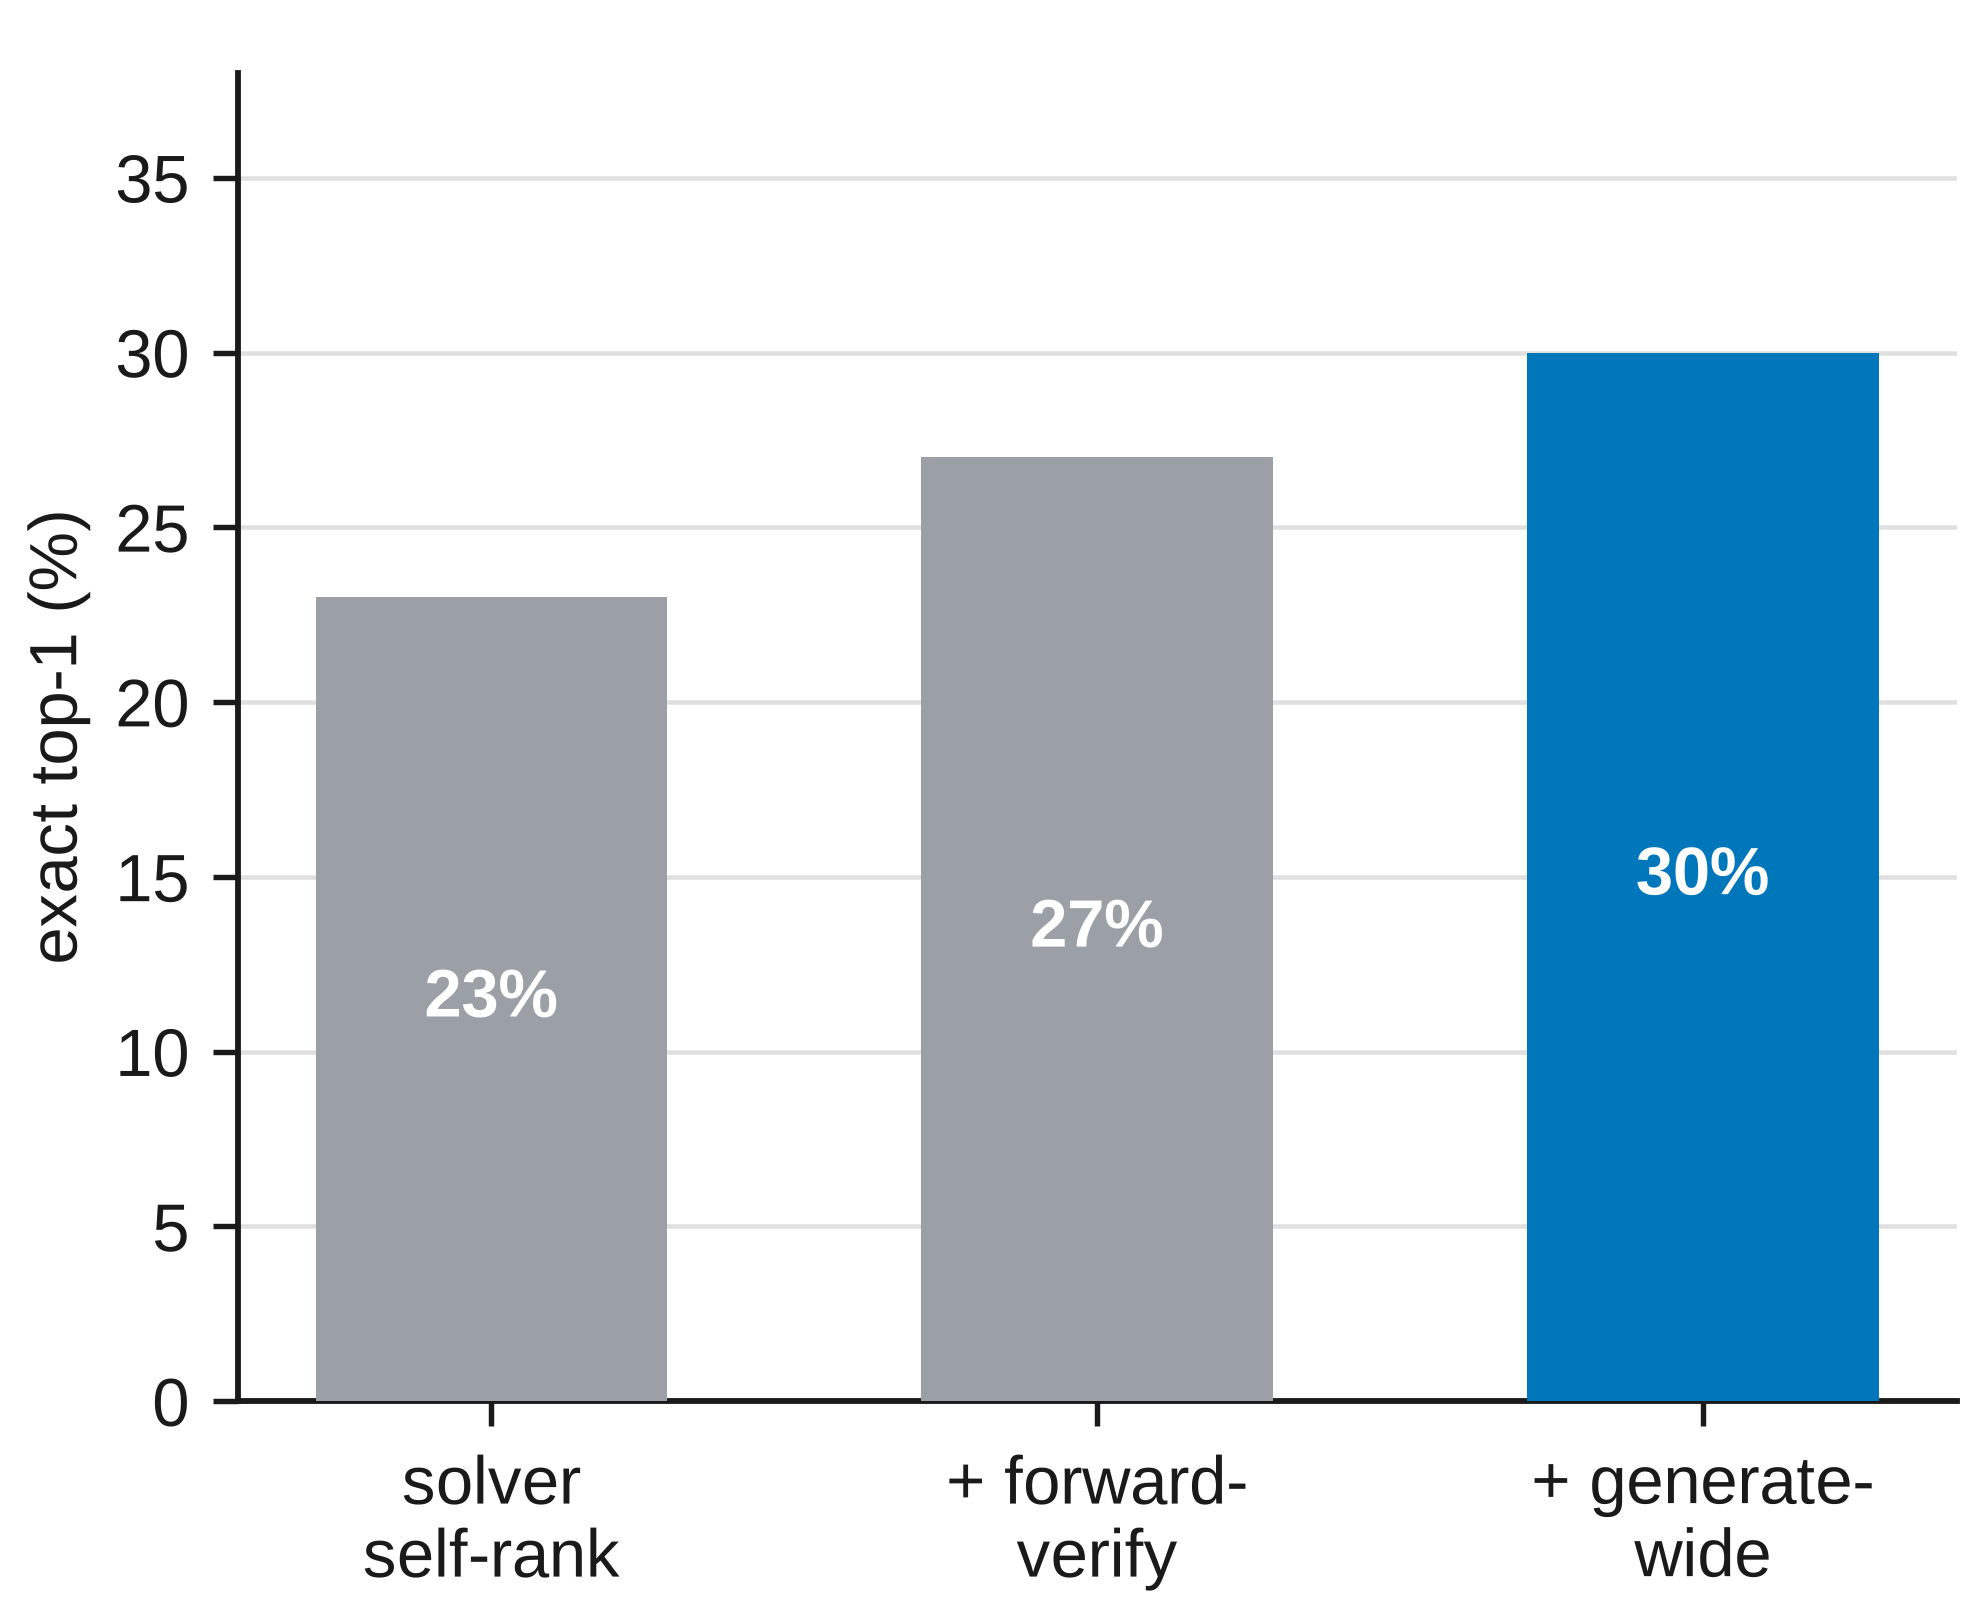
\includegraphics[width=0.52\linewidth]{fig3_method.png}
  \caption{Inference ladder on the 60-compound arm: 23\% $\to$ 27\% $\to$ 30\% top-1.
  Generate-wide lifts recall (32\% $\to$ 42\%); the wall is proposal, not ranking.}
  \label{fig:fig3-method}
\end{figure}

\paragraph{Non-LLM verifiers.}
On the same candidate sets, a HOSE-style lookup ties self-ranking; a modest GNN reaches
59/65 (91\%) vs the LLM verifier's 58/65 (89\%) --- directional.
Deranging observed $^{13}$C pairings collapses precision ($p{=}0.001$).
A small IRexp-fine-tuned generator pooled with Claude lifts locked-slice recall 33.5\% $\to$ 54.1\% and
top-1 28.4\% $\to$ 35.1\% (McNemar $p{=}0.015$), showing the wall is a property of
\textbf{training-free elicitation}, not of the task.

\subsection{Decomposition across published literature}
\label{sec:literature}

Any system reporting top-1 $= a$ and top-$k = b$ implies recall $\geq b$ and conditional
precision $\leq a/b$.
Applying this to published figures (\texttt{scripts/literature\_decomposition.py}):

\begin{table}[ht]
\caption{Selected literature decomposition rows (connectivity-scored or as published).}
\label{tab:lit-decomp}
\centering
\scriptsize
\setlength{\tabcolsep}{3pt}
\begin{tabular}{@{}p{2.6cm}p{2.4cm}rrrr@{}}
\toprule
system & data ($n$) & top-1 & top-$k$ ($k$) & recall & prec. \\
\midrule
this work, solver alone & literature (300) & 39.3\% & 44.3\% (3) & 44.3\% & 88.7\% \\
this work + forward-verify & literature (194) & 29.9\% & 33.5\% (3) & 33.5\% & \textbf{89.2\%} \\
NMR-Solver~\citep{jin2025nmrsolver} & literature (450) & 52.9\% & 67.3\% (10) & $\geq$67.3\% & $\leq$78.6\% \\
NMRAgent~\citep{fang2026nmragent} & literature (450) & 61.6\% & 70.0\% (10) & $\geq$70.0\% & $\leq$88.0\% \\
Espejo Morales~\citep{espejo2026agentic} & education (236) & 80.9\% & 90.0\% (5) & $\geq$90.0\% & $\leq$89.9\% \\
Espejo Morales~\citep{espejo2026agentic} & industrial (34) & 20.6\% & 29.1\% (5) & $\geq$29.1\% & $\leq$70.9\% \\
Alberts, 6--13 atoms~\citep{alberts2025benchmarks} & NIST IR (3,455) & 63.8\% & 84.0\% (10) & 84.0\% & 75.9\% \\
SpecX, scaffold split~\citep{xiang2026specx} & simulated (99,439) & 29.7\% & 50.6\% (10) & 50.6\% & 58.7\% \\
\bottomrule
\end{tabular}
\end{table}

\textbf{Three groups changed only the data}, and recall carried \textbf{68\%} (NMR-Solver
simulated $\to$ real), \textbf{70\%} (SpecX random $\to$ scaffold) and \textbf{83\%}
(Espejo education $\to$ industrial) of each collapse.
Recall binds where spectra are real and heterogeneous; ranking dominates on simulated or
single-library data.
The solver-alone precision column on $n{=}300$ is self-ranking (118/133); the
forward-verify row is the instrumented $n{=}194$ slice (58/65) --- not interchangeable.

\subsection{Pre-registered expansion, pooled headline, and scale roadmap}
\label{sec:expansion}

The $n{=}300$ headline is the pre-registered pool of the locked 194 and a 106-compound
expansion draw (Table~\ref{tab:slices}; Appendix Tables~\ref{tab:expansion},~\ref{tab:clean295}).
Five $^{13}$C-overread flags (R12, R22, R25, R82, R91) stay in the 300; validate-clean is
116/295 (39.3\%) top-1 / 130/295 (44.1\%) recall.
The expansion slice is easier (59.4\% vs 28.4\% top-1) --- disclosed, not hidden.
A Fable arm is incomplete (68/106; not scored; never pooled).
Figure~\ref{fig:fig-wall} and Table~\ref{tab:fverify} remain the $n{=}194$ instrumented
forward-verified diagnosis; expansion-106 fverify was \textbf{not} run.

\paragraph{Scale roadmap / larger blind round.}
A second pre-registered draw toward $n{\approx}500$ (230 compounds; 115/115 simple/complex;
six $^{13}$C-overread flags known \emph{before} any solve) now has \textbf{230/230} Opus
deposits and a frozen 690-candidate file.
Scoring is \textbf{deferred}: the answer key is withheld, no top-1 or recall exists, and
forward-verify was not run on this round.
Those deposits used a thinking-tier consumer arm and are not interchangeable with the
no-thinking $n{=}300$ protocol until scored under a declared contract.
This round is \textbf{not} pooled into the headline and is not a wall figure.

\section{Discussion}
\label{sec:discussion}

Frontier LLMs are \textbf{good verifiers} ($\approx$89\% conditional precision on the
$n{=}194$ instrumented slice) and \textbf{weak proposers} (44\% generation recall on
$n{=}300$; 34\% on the instrumented 194) on real literature peak lists --- propose $\gg$
verify, not the reverse.
The primary research contribution is the \textbf{benchmark + stage decomposition +
contamination/cross-vendor diagnosis}, not a solved elucidator and not a Data Descriptor
for IRexp.
The expansion slice scored higher than the locked 194 (Section~\ref{sec:expansion}); pooling
does not erase that gap.
The $n{\approx}500$ deposits do not yet change any scored number.

\paragraph{Reporting contract.}
External work on IRSpectra-Bench should deposit ranked SMILES under the released protocol and
report, at minimum: (i) top-1 constitution, (ii) generation recall, (iii) verification
precision $|$ recall, with bootstrap CIs and candidate budget.
Top-1 alone conflates the two stages.
Nonsignificant ladder gains (forward-verification vs self-ranking, $p{=}0.55$; generate-wide
top-1, $p{=}0.34$) should be cited as \textbf{diagnostic}, not as accuracy advances.
Corpus-reweighted top-1 (\textbf{26.5\%} on the validate-clean subset) is the better estimate
for an arbitrary literature draw.
Training is not foreclosed: IRexp fine-tuning lifts recall to 54\%.
Those gains compound with open experimental data, honest benchmarks, and inference scaffolding that
transfers to each new model.

\subsection{Implications for agentic elucidation}
\label{sec:agentic}

The diagnosis implies an \textbf{asymmetric pipeline}, not another verifier stacked on a thin
pool.
Proposal is the expensive stage: diversity, tool-use into enumeration / database search /
formula-constrained decode, or generate-wide sampling that actually enlarges the pool.
Verification is cheap: once the true constitution is proposed, training-free
forward-verification selects it $\approx$89\% of the time on the instrumented $n{=}194$
slice (58/65).
Spending the budget on a second ranker cannot recover the 129/194 compounds that were never
proposed.

IR-Agent-style table-interpretation and retrieve tools~\citep{noh2025iragent} are complementary
\emph{feature} agents --- they improve how a spectrum is read and how a given pool is
re-ranked.
MolQuest- and Espejo-style architecture search~\citep{han2026molquest,espejo2026agentic}
still needs this stage contract: a better reader that does not change
$P(\text{true}\in\text{pool})$ cannot move top-1 on a recall-bound bench.
The next ICLR-relevant agent is a \textbf{proposer}, not a second verifier:
formula-constrained generators, fragment assembly, and search that change that probability.
We are \textbf{not} shipping another ChemCrow-for-IR or a SpectraLLM-style fine-tune:
the bench is a reporting contract so external agents can be compared honestly on the same
object.
Multi-modal agents raise recall only if they enlarge the pool.
Training on open experimental corpora (IRexp as the pointer, not this paper's object) is the
one intervention we have already seen move recall (33.5\% $\to$ 54.1\% on the locked slice).
Nonsignificant ladder steps are \textbf{diagnostic}, not accuracy claims
(forward-verification vs self-ranking McNemar $p{=}0.55$; generate-wide top-1 $p{=}0.34$):
re-ranking is the wrong primary bet and does not license a solved-elucidator headline.

\section{Limitations}
\label{sec:limitations}

Scoring is mechanical; solver runs were transcript-audited for zero ground-truth access.
\textbf{(i) Consumer harness.} Claude Opus via consumer subscription; no model snapshot,
temperature, seed, or thinking tier. Exact inference is not reproducible; scoring is.
Batch instruction text was not captured --- only per-compound payloads are released.
We do \textbf{not} recommend thinking-high follow-ups as a path to a method result.
\textbf{(ii) Pretraining contamination} is bounded by formula-only (23\% $\to$ 5\%) and flat
recency but \textbf{not excluded}; verbatim spectral strings from PMC in the prompt remain a
retrieval confound.
\textbf{(iii) Object type, formula and scoring.} Band/shift lists, not raw traces; formula
supplied (as from HRMS) --- absolute accuracies are not interchangeable with no-formula
systems. Headline metrics score constitution; with stereochemistry, top-1 is 93/295 (31.5\%)
on the validate-clean subset.
\textbf{(iv) Statistical honesty.} Forward-verification vs self-ranking unresolved ($p{=}0.55$);
generate-wide top-1 likewise ($p{=}0.34$). Four-model comparison at $n{=}24$ underpowered for
adjacent ranks with disclosed protocol asymmetry. The inference ladder \textbf{diagnoses a
bottleneck}; it is not a demonstrated accuracy advance.
\textbf{(v) No method SOTA chase.} SpectraLLM, IR-Agent, Spectro, NMIRacle, Alberts IR
transformers and CASE were \textbf{not scored} on IRSpectra-Bench. The contribution is the
bench and the proposal$\ll$verification split, not a claim that an off-the-shelf LLM beats
trained elucidators.
\textbf{(vi) Expansion difficulty gap; fverify not on 106 or 230.} Expansion top-1 is 59\% vs 28\%
on the locked 194; pooling to $n{=}300$ does \textbf{not} hide that gap
(Table~\ref{tab:slices}). Figure~\ref{fig:fig-wall} and 58/65 are the locked $n{=}194$
instrumented slice; forward-verify was not run on the 106 or on the 230-compound
$n{\approx}500$ deposits. The $n{\approx}500$ round is deposited (230/230) and
\textbf{unscored} --- no top-1 --- and used a thinking-tier consumer arm, so it is not a
no-thinking replication. Headline $n{=}300$ is Claude Opus generation (no thinking
tier); four-vendor replication is on 60 compounds; candidate budgets differ.
A Fable expansion arm is incomplete (68/106) and is not pooled.
\textbf{(vii) Deferred arms.} Expert-chemist audit formally deferred (not run).
Leave-one-modality-out abandoned. Extraction-recall human audit of the mining parser is
deferred to the \textit{Scientific Data} companion.
\textbf{(viii) Scope.} Battery subset uses literature electrolyte chemistry, not operando
spectra; single-sample scoring per compound; organic literature bias of PMC-OA sources.
Short answers to the same attacks are collected in Appendix~\ref{app:faq}.

\section{Conclusion}
\label{sec:conclusion}

IRSpectra-Bench makes LLM structure elucidation from literature peak lists \textbf{measurable
and decomposable}.
On the pooled generation cohort ($n{=}300$), a frontier LLM recovers 39\% top-1 and 44\%
generation recall; corpus-reweighted top-1 is 27\%.
Propose $\gg$ verify: generation recall --- not verification --- binds end-to-end accuracy
(forward-verified on the locked $n{=}194$ slice); the diagnosis replicates across
vendors and is recovered from published top-$k$ figures.
We release frozen predictions and a mechanical scorer so others can report the same three
numbers.
The band-list resource behind the bench is documented separately as a
\textit{Scientific Data} Data Descriptor (in preparation)~\citep{yabbarov2026irexp}.

\section*{AI use statement}
Frontier LLMs were used as \textbf{experimental solvers} under the consumer harness in
Sections~\ref{sec:setup}--\ref{sec:results} (Claude Opus on the headline cohort; three
other vendor families on the 60-compound arm), not as a substitute for author analysis,
scoring, or claim-checking.
Inference used no thinking tier and no pinned model snapshot.
We did not use generative AI to invent or alter reported metrics.
Generative tools assisted manuscript editing and formatting; the authors reviewed the text
and take responsibility for all claims, including any AI-assisted wording.

\section*{Ethics statement}
This work evaluates publicly available open-access literature peak lists and commercial LLM
APIs under consumer terms.
No human-subject data.
We do not claim clinical or regulatory readiness for automated elucidation.
Licensing of redistributed numeric extractions is documented in the companion Data Descriptor
and dataset notices (PMC-OA terms are mixed --- not uniformly CC-BY; Chemotion is CC-BY-SA).

\section*{Reproducibility statement}
Every training-free number regenerates from released questions, answers, frozen predictions
and scripts in the code release.
The sampler, InChIKey scorer and forward-verification harness are scripted end-to-end.
Consumer-harness inference cannot be bit-exact replayed (Section~\ref{sec:limitations});
distributional agreement is the intended claim.
Fine-tuning against the bench should use \texttt{data/train\_no\_bench.jsonl.gz} so benchmark
InChIKeys are withheld.

\enlargethispage{5\baselineskip}
\section*{Acknowledgements}
We acknowledge support from the Natural Sciences and Engineering Research Council of Canada (NSERC) through a CREATE training program. Institutional details and named funding references are omitted for double-blind review and will be restored in the camera-ready version.
\bibliography{references}
\bibliographystyle{iclr2027_conference}

\appendix

\section{Dataset pointer (IRexp)}
\label{app:dataset}

IRexp is \textbf{not} re-described here as a Data Descriptor.
During double-blind review, the commercial redistributable pool is available from an anonymised review copy (no author-identifying host):
\begin{itemize}
  \item Anonymised dataset copy: \url{https://anonymous.4open.science/r/peaklist-corpus-review-10C4/}
  \item Companion manuscript: anonymised \textit{Scientific Data} Data Descriptor (in preparation)~\citep{yabbarov2026irexp}
\end{itemize}
Named archival hosting will replace the review copy in the camera-ready version.
File schema and aggregate counts ship with that copy (\texttt{SCHEMA.md}, \texttt{data/}).

Benchmark construction details beyond Section~\ref{sec:benchmark} (spectral validation
filters, prompt-leakage audit, electrolyte SMARTS) ship with the code release and the
companion Data Descriptor~\citep{yabbarov2026irexp}; they are not re-presented here.

\section{Reviewer FAQ}
\label{app:faq}

These answers restate Limitations~\ref{sec:limitations}; they add no new metrics.

\textbf{Why is top-1 39\% if the wall figure looks worse?}
Headline generation is $n{=}300$ (118/300 top-1; 133/300 recall).
Figure~\ref{fig:fig1}c and Figure~\ref{fig:fig-wall} are the locked $n{=}194$
forward-verified slice (58/7/129). Do not read the wall as a pooled $n{=}300$
diagnosis.

\textbf{Is the expansion hidden in the pool?}
No. Expansion top-1 is 59\% vs 28\% on the locked 194 (Table~\ref{tab:slices}).
That gap is a result.

\textbf{Where is forward-verify on the 106?}
Not run. Conditional 89\% (58/65) is $n{=}194$ only.
Do not invent a pooled $n{=}300$ wall.

\textbf{Where is the $n{\approx}500$ top-1?}
Nowhere. A 230-compound blind round is deposited (230/230; 690 candidates);
scoring is deferred (key withheld). Deposit counts are not accuracy.
Headline stays $n{=}300$. Those deposits used a thinking-tier arm and are not
interchangeable with the no-thinking protocol.

\textbf{Consumer harness / no snapshot / no thinking tier?}
Correct and intentional for the scored headline. Scoring of frozen deposits is
reproducible; inference is not bit-exact. We do not recommend thinking-high
experiments as a revision path for a method result.

\textbf{Why no SpectraLLM / IR-Agent / CASE SOTA table?}
Different objects (simulated or NIST IR; trained agents; exhaustive enumerators).
None is scored on this bench. The paper is a stage diagnosis, not a method race.

\textbf{Is IRexp a second ICLR paper?}
No. IRexp is a companion resource pointer (Appendix~\ref{app:dataset};
Figure~\ref{lst:payload}).
Corpus construction belongs in the \textit{Scientific Data} descriptor.

\section{Extended tables and figures}
\label{app:extended}

This conference version keeps the protocol plate
(Figure~\ref{fig:fig1}), chemistry space
(Figure~\ref{fig:fig-chemspace}), Listing~1 payload (Figure~\ref{lst:payload}),
robustness (Figure~\ref{fig:fig-robustness}), the
forward-verification mechanism (Figure~\ref{fig:fig-mechanism}), and the inference
ladder (Figure~\ref{fig:fig3-method}).
The diagnosis wall on the $n{=}194$ instrumented slice is repeated below
(Figure~\ref{fig:fig-wall}) so the lead figure is not the only copy.
Additional archive plates are omitted here; they do not change the pooled $n{=}300$
generation headline or the $n{=}194$ instrumented wall.

\begin{figure}[h]
  \centering
  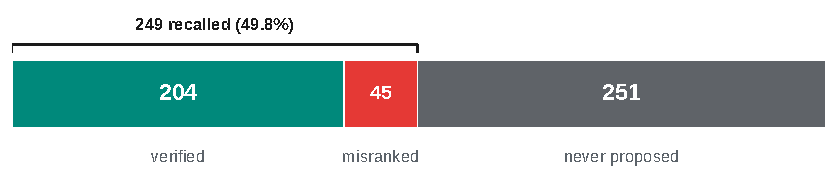
\includegraphics[width=0.92\linewidth]{fig_wall.pdf}
  \caption{Diagnostic wall: \textbf{locked $n{=}194$ instrumented slice}
  (58 verified / 7 mis-ranked / 129 never proposed).
  Expansion-106 has no forward-verify; this is \textbf{not} a pooled $n{=}300$ wall.
  Headline generation recall is 133/300.
  Never-proposed cases bind top-1 despite 89\% conditional precision (58/65).
  Same slice as Figure~\ref{fig:fig1}c.}
  \label{fig:fig-wall}
\end{figure}

\begin{table}[h]
\caption{Locked $n{=}194$ cases from released candidate files.
$^{13}$C chamfers in ppm; Tanimoto Morgan $r{=}2$. IDs are locked-round labels.}
\label{tab:cases}
\centering
\scriptsize
\setlength{\tabcolsep}{3.5pt}
\begin{tabular}{@{}lp{2.15cm}p{8.75cm}@{}}
\toprule
mode & id / formula & what failed \\
\midrule
\textbf{Proposal miss} &
main-R06 / C$_{29}$H$_{30}$FNO$_{2}$ &
True acridinedione never in the 3-candidate pool (Tanimoto-0.90 regioisomer: 4-fluorophenyl/phenyl swapped).
IR 1641, 1510~cm$^{-1}$; $^{13}$C 195.7. Verifier unused. \\
\textbf{Verify-save} &
v3-R25 / C$_{10}$H$_{14}$N$_{2}$O &
True 2-pyridyl picolinamide at self-rank 3; self-rank 1 is 3-pyridyl.
Forward-verify recovers (chamfer 0.42 vs 1.30~ppm). IR 1679~cm$^{-1}$.
Fig.~\ref{fig:fig-mechanism}. \\
\textbf{Verify-fail} &
v3-R26 / C$_{14}$H$_{11}$N$_{3}$O$_{3}$ &
True 3-nitrophenyl dihydroquinazolinone in pool (self-rank 2); 2-nitro ranked first.
Chamfer 1.35 vs 1.36~ppm. IR 1652, 1530, 1352~cm$^{-1}$. \\
\bottomrule
\end{tabular}
\end{table}

\begin{table}[h]
\caption{Expansion round (Claude Opus, InChIKey-14). Five $^{13}$C-overread flags stay in
the $n{=}300$ headline; validate-clean $n{=}295$ in Table~\ref{tab:clean295}.
Incomplete Fable arm (68/106) is never pooled.}
\label{tab:expansion}
\centering
\begin{tabular}{@{}lrr@{}}
\toprule
 & all ($n{=}106$) & clean ($n{=}101$) \\
\midrule
top-1 & 63/106 (59.4\%) & 61/101 (60.4\%) \\
generation recall & 68/106 (64.2\%) & 65/101 (64.4\%) \\
\bottomrule
\end{tabular}
\end{table}

\begin{table}[h]
\caption{Validate-clean sensitivity ($n{=}295$; five $^{13}$C-overread flags excluded).
Same scorer as Table~\ref{tab:headline}; not the headline.}
\label{tab:clean295}
\centering
\scriptsize
\setlength{\tabcolsep}{3pt}
\begin{tabular}{@{}lrrr@{}}
\toprule
metric & overall ($n{=}295$) & simple ($n{=}147$) & complex ($n{=}148$) \\
\midrule
top-1 exact constitution & 116/295 (39.3\%) [34--45] & 59.2\% [51--67] & 19.6\% [14--26] \\
recovered (top-3) & 130/295 (44.1\%) [39--49] & 63.9\% [56--71] & 24.3\% [17--31] \\
scaffold-level (best Tanimoto $\geq 0.45$) & 64\% & 80\% & 48\% \\
mean best Tanimoto & 0.66 & 0.79 & 0.53 \\
\bottomrule
\end{tabular}
\end{table}

By size on $n{=}295$: 67.9\% top-1 at $\leq$15 heavy atoms, 42.8\% at 16--25, 16.7\% above 25
($n{=}53/152/90$).
Full InChIKey (stereo): 93/295 (31.5\%) top-1 [26--37], recall 108/295 (36.6\%) [31--42].
Corpus-reweighted (17.5\% simple / 82.5\% complex): top-1 \textbf{26.5\%} [21--32], recall
\textbf{31.3\%} [25--37].
Self-ranking precision $|$ recall: 116/130 (89.2\%).

\end{document}
 shim for older compile notes.
% main_IRExpBench_only.tex is an optional orphan alternate --- not the ICLR build root.
% Headline n=300 generation (194 locked + all 106 expansion); fig_wall is the n=194 instrumented slice.
% expand-500: 230/230 deposited, unscored --- do not invent top-1 or a pooled wall.
% Compile with pdfLaTeX or XeLaTeX + BibTeX (references.bib + iclr2027_conference.bst).
% \iclrfinalcopy is the only official sty flag that prints \author and drops
% the left-margin submission ruler (see tex/iclr2027_conference.sty).
\documentclass{article}
\usepackage{iclr2027_conference,times}

\usepackage{hyperref}
\usepackage{url}
\usepackage{booktabs}
\usepackage{graphicx}
\usepackage{amsmath,amssymb}
\usepackage{enumitem}
\usepackage{placeins}
\usepackage{xcolor}
\usepackage{listings}
\usepackage{framed}
\lstdefinestyle{benchjson}{
  basicstyle=\ttfamily\scriptsize,
  breaklines=true,
  columns=fullflexible,
  keepspaces=true,
  showstringspaces=false,
  frame=none,
  literate={-}{-}1
}
\setlist{nosep,leftmargin=1.35em}
\setlength{\textfloatsep}{10pt plus 2pt minus 2pt}
\setlength{\floatsep}{8pt plus 2pt minus 2pt}
\setlength{\intextsep}{8pt plus 2pt minus 2pt}

\graphicspath{{figures/}{../figures/}{./}}

% Alternate Overleaf title (not used): Molecular Structure Elucidation with Frontier Models: A Benchmark on Literature-Reported IR, $^1$H, and $^{13}$C NMR Peak Lists
\title{Generation Recall, Not Verification, Binds LLM Structure Elucidation from Literature Spectra}

\author{
Ilkham Yabbarov\textsuperscript{1,$\dagger$},
Rudra Sondhi\textsuperscript{1},
Rodrigo A.\ Vargas-Hern\'andez\textsuperscript{1,2,3,$\dagger$}\\
\textsuperscript{1}Department of Chemistry and Chemical Biology, McMaster University,
Hamilton, Ontario L8S 4L8, Canada.\\
\textsuperscript{2}Brockhouse Institute for Materials Research, McMaster University,
Hamilton, Ontario L8S 4L8, Canada.\\
\textsuperscript{3}School of Computational Science and Engineering, McMaster University,
Hamilton, Ontario L8S 4L8, Canada.\\
$\dagger$\,\textit{E-mail:} yabbaroi@mcmaster.ca, vargashr@mcmaster.ca
}

\newcommand{\fix}{\marginpar{FIX}}
\newcommand{\new}{\marginpar{NEW}}

% Official ICLR 2027 switch: show \author and disable the submission linenumber
% ruler. The same flag also sets the running header to "Published as...".
% Double-blind (submit): keep \iclrfinalcopy commented; \maketitle then prints
% "Anonymous authors / Paper under double-blind review". Camera-ready: uncomment
% \iclrfinalcopy and delete the \lhead override below.
% \iclrfinalcopy  % OFF for double-blind submission; re-enable for camera-ready
\begin{document}

\maketitle
\lhead{Under review as a conference paper at ICLR 2027}

\begin{abstract}
Frontier large language models are often cast as near-solved structure elucidators on
curated spectra. We ask the operational question: given only the molecular formula and
\textbf{literature-reported} IR / $^1$H / $^{13}$C \textbf{peak lists} --- not digitised
traces --- can an off-the-shelf LLM recover constitution, and \textbf{which stage fails}
when it cannot?

The binding claim is \textbf{propose $\gg$ verify}: candidate proposal, not ranking,
is the expensive stage.
We release \textbf{IRSpectra-Bench}, a blind peak-list benchmark of \textbf{300}
compounds (194 locked $+$ all 106 Opus expansion, flags included) drawn from the
companion \textbf{IRexp} band-list resource~\citep{yabbarov2026irexp} --- cited
here, not re-described --- with a fixed RDKit InChIKey-connectivity contract and
decomposable \textbf{generation recall} / \textbf{verification precision} metrics.
A frontier LLM recovers \textbf{39\%} top-1 (118/300; 95\% CI 34--45), or
\textbf{27\%} after corpus reweighting; generation recall is \textbf{44\%} (133/300).
On the forward-verified $n{=}194$ slice the true structure enters the pool for only
\textbf{34\%} of compounds, yet training-free forward-verification selects it
\textbf{89\%} of the time once proposed (58/65).
The expansion slice is easier (59\% vs 28\% top-1) and is disclosed, not hidden.
A larger deposited blind round toward $n{\approx}500$ is \textbf{unscored} and is
not in this headline.
The same recall $\ll$ precision asymmetry replicates across \textbf{four vendor families}.
Formula-only controls collapse; accuracy is flat in source-paper year; generate-wide
sampling lifts recall where verification alone barely moves top-1.
Recovered from published top-$k$ figures, recall carries \textbf{68--83\%} of the accuracy
collapse from curated or simulated spectra to real heterogeneous peak lists.
Frozen predictions, scorers and code are released for mechanical re-evaluation.
\end{abstract}

\section{Introduction}
\label{sec:introduction}

Structure elucidation from spectra sits at the centre of synthetic and analytical chemistry,
and machine learning increasingly treats it as a sequence or agent task.
Encoder--decoder models train on paired corpora~\citep{chacko2024spectro,ottomano2025nmiracle,alberts2024ir};
LLM agents and puzzle benches report high recovery on curated or education
spectra~\citep{kamber2026chemist,guo2024molpuzzle,zhuang2025treesearch,espejo2026agentic}.
Cross-paper numbers swing wildly with harness (e.g.\ GPT-4o from 1.4\% to 57.8\% on MolPuzzle
under different prompting~\citep{guo2024molpuzzle,zhuang2025treesearch}).
What remains under-measured is the harder operational task: \textbf{taking peak lists as
printed in open-access papers and recovering constitution} with an off-the-shelf model,
a fixed molecular-representation scoring contract, and an honest account of
\textbf{which stage of elucidation binds} --- proposal versus verification.

We argue that end-to-end top-1 alone is the wrong reporting primitive.
Any system that returns a ranked candidate list factorises as
\begin{equation}
\text{top-1} \;=\; \underbrace{P(\text{true} \in \text{pool})}_{\text{generation recall}}
\times
\underbrace{P(\text{rank}=1 \mid \text{true} \in \text{pool})}_{\text{verification precision}}.
\end{equation}
These rates have different denominators and must not be differenced.
Prior work already notes that re-ranking cannot recover a missing
candidate~\citep{priessner2026reasoning}; we supply the missing \textbf{measurement
infrastructure at scale}.

\paragraph{Contributions.}
\begin{enumerate}
  \item \textbf{IRSpectra-Bench} --- a blind, complexity-stratified peak-list benchmark ($n{=}300$)
        with a pre-registered InChIKey-connectivity scorer and community reporting contract
        (top-1, generation recall, verification precision $|$ recall).
  \item \textbf{A recall-bound diagnosis} on a frontier LLM: propose $\gg$ verify.
        Generation recall is 44\% on the pooled $n{=}300$ cohort; on the $n{=}194$
        instrumented slice, 34\% proposed and 89\% selected once proposed; that slice's
        top-1 moves only 28\% $\to$ 30\% under training-free forward-verification.
  \item \textbf{Contamination and cross-vendor controls} --- formula-only and recency bounds;
        four-vendor replication of recall $\ll$ precision.
  \item \textbf{A literature decomposition} that recovers the same split from published top-$k$
        figures, showing recall carries most of the collapse on real heterogeneous data.
\end{enumerate}

\paragraph{Dataset pointer (resource, not co-headline).}
Band lists come from the companion \textbf{IRexp} resource (121,233 records; 43,060
structure-linked; 33,201 full IR+$^1$H+$^{13}$C+structure quadruples); an anonymised
review copy is in Appendix~\ref{app:dataset}.
Construction and licensing live in a \textit{Scientific Data} manuscript (in
preparation)~\citep{yabbarov2026irexp}.
This ICLR paper \textbf{cites} that resource and does not re-present a Data Descriptor.

\begin{figure}[t]
  \centering
  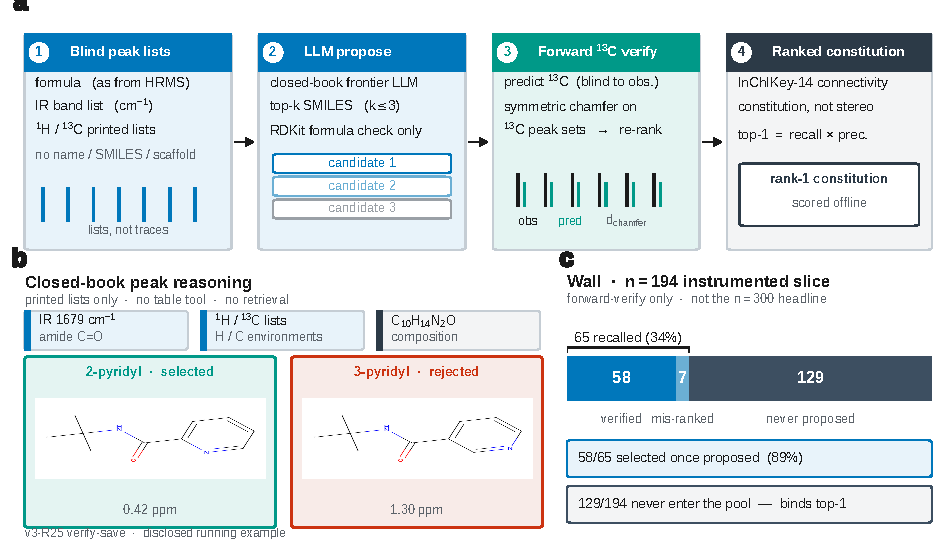
\includegraphics[width=\linewidth]{fig1_overview.pdf}
  \caption{IRSpectra-Bench protocol.
  (a)~Printed IR/$^1$H/$^{13}$C lists $+$ formula $\rightarrow$ closed-book LLM
  proposes top-$k$ SMILES (RDKit formula check) $\rightarrow$ forward $^{13}$C
  (blind) $\rightarrow$ chamfer re-rank $\rightarrow$ InChIKey-14.
  (b)~Evidence is the lists themselves (no peak-table tool, no retrieval).
  Running example v3-R25 (IR 1679~cm$^{-1}$; chamfer 0.42 vs 1.30~ppm).
  (c)~Locked $n{=}194$ instrumented wall: 58 verified / 7 mis-ranked / 129 never
  proposed. \textbf{Not} a pooled $n{=}300$ wall
  (headline generation: Table~\ref{tab:headline}; diagnostic repeat:
  Figure~\ref{fig:fig-wall}).}
  \label{fig:fig1}
\end{figure}

\section{Related work}
\label{sec:related-work}

\paragraph{Trained spectra $\to$ structure models.}
Sequence and graph decoders on paired
corpora~\citep{chacko2024spectro,hu2024multitask,yang2026nmrtrans,ottomano2025nmiracle,alberts2024ir,alberts2025benchmarks}
are accurate in-distribution but typically scored end-to-end.
We do not claim to beat them on IRSpectra-Bench; Spectro, NMIRacle, Alberts IR transformers
and CASE are \textbf{not yet scored} on our bench (Section~\ref{sec:limitations}) --- a gap we
state honestly and leave to the released scorer.

\paragraph{Agentic elucidation: three regimes.}
The contrast is the \textbf{setting and the stage split}, not a method scoreboard.
(i)~\emph{Tool-using lab agents} --- ChemCrow~\citep{mbran2024chemcrow},
Coscientist~\citep{boiko2023coscientist} --- show that LLMs can call instruments and
planners; they do not measure which elucidation stage binds.
(ii)~\emph{Spectrum-native agents} improve \emph{how} a model reads a spectrum or
re-ranks a \textbf{fixed} pool: tree-search~\citep{zhuang2025treesearch},
SpecMol~\citep{shen2025specmol}, Priessner \textit{et al.}~\citep{priessner2026reasoning},
NMR-Solver~\citep{jin2025nmrsolver}, NMRAgent~\citep{fang2026nmragent}.
Priessner already notes that re-ranking cannot recover a missing candidate; we measure
that failure at literature-peak-list scale.
SpectraLLM~\citep{su2025spectrallm} is a \textbf{fine-tuned} multi-spectral elucidator
on \textbf{simulated} corpora (QM9S DFT; Alberts USPTO multimodal) --- a different object
and a different training regime; we do not score it here.
IR-Agent~\citep{noh2025iragent} (ICLR 2026) is the closest concurrent multi-agent IR
elucidator: on \textbf{NIST experimental IR} a translator proposes a SMILES pool, TI+Ret
enrich local (peak-table) and global (retrieved-spectrum) features, and an SE expert
re-ranks (Top-$k$ SMILES; atom type / scaffold / carbon count may be prompt-injected).
(iii)~\emph{Agentic-search benches} --- MolQuest~\citep{han2026molquest},
NMRGym~\citep{fang2026nmrgym}, Espejo Morales \textit{et al.}~\citep{espejo2026agentic}
(education $\to$ industrial instrument files: 80.9\% $\to$ 20.6\%) --- ask which
architecture or abductive loop wins.
IRSpectra-Bench is the harder operational object: \textbf{literature peak lists}
(IR+$^1$H/$^{13}$C+formula as from HRMS), \textbf{off-the-shelf} closed-book models, no
name, SMILES, or scaffold hint.
We measure \textbf{which stage binds} after spectra are read --- generation recall versus
verification precision $|$ recall --- on pooled $n{=}300$, with instrumented
forward-verify on $n{=}194$.
IR-Agent's SE expert over a \textbf{fixed candidate pool} is exactly the regime our
ladder diagnoses as recall-limited (proposal binds; conditional forward-verify
$\approx$89\%, 58/65).
TI+Ret can enrich \emph{features} but does \textbf{not} remove a proposal wall if the true
structure never enters the pool.
Architecture search that does not change $P(\text{true}\in\text{pool})$ cannot move
top-1 on a recall-bound bench.
We do not claim to beat SpectraLLM or IR-Agent on their native sets; neither is scored
here.
\begin{center}
\scriptsize
\setlength{\tabcolsep}{4pt}
\begin{tabular}{@{}llll@{}}
\toprule
 & input & metric & binds \\
\midrule
IR-Agent & NIST experimental IR & Top-$k$ SMILES & re-rank given pool \\
this paper & lit.\ IR+$^1$H/$^{13}$C+formula lists & recall vs prec.$|$recall & proposal \\
\bottomrule
\end{tabular}
\end{center}

\paragraph{Heterogeneous data, CASE, and positioning.}
Most prior suites use simulated or single-instrument spectra; we use literature-reported
peak lists across thousands of laboratories and report formula-only and recency controls
(Section~\ref{sec:contamination}).
Matching predicted to observed shifts --- DP4~\citep{smith2010dp4},
CASE~\citep{elyashberg2012case}, NMR-Solver, NMRAgent --- is easier than inverse
generation; CASE enumerators have exhaustive recall by construction, while the LLM
literature almost never reports whether the true structure was proposed at all.
SpecX~\citep{xiang2026specx} bounds a related multi-modal spectroscopy task on
simulated traces.
IRSpectra-Bench is an openly redistributable literature-peak-list suite with a
\textbf{stage decomposition}, measured on Claude and replicated across three other
model families.

\FloatBarrier
\section{IRSpectra-Bench}
\label{sec:benchmark}

\subsection{Task and inputs}

Each of 300 problems supplies the \textbf{molecular formula} (as from HRMS), the \textbf{IR
band list} (cm$^{-1}$), and \textbf{$^1$H / $^{13}$C shift lists} --- exactly the textual form
reported in open-access papers.
No name, SMILES or scaffold hint.
Inputs are author-transcribed \textbf{band and shift lists}, not absorbance traces or FIDs:
a different object from digitised-spectrum benchmarks~\citep{espejo2026agentic}, and one that
matches how language models consume literature.

The cohort is the pre-registered pool of a locked 194 (spectrally validated main round 134 $+$
60 controls) and a 106-compound expansion draw ($n{=}300{=}194{+}106$).
Five expansion records fail the same $^{13}$C-overread audit used on the main round and are
included in the 300 (validate-clean $n{=}295$ in Appendix~\ref{app:extended}).
Problems are drawn from the structure-complete split of IRexp (\texttt{irexp\_resolved}; see
companion Data Descriptor)~\citep{yabbarov2026irexp}.
On the locked 194, author peak assignments name a ring system in 10/194; those are solved
1/10 vs 54/184 for the rest, so named-ring annotation does not drive that slice.
Figure~\ref{fig:fig-chemspace} summarises the chemistry space of the pooled headline.
Figure~\ref{lst:payload} is the solver-facing contract: formula plus printed peak lists,
gold constitution held out.

\begin{figure}[ht]
  \centering
  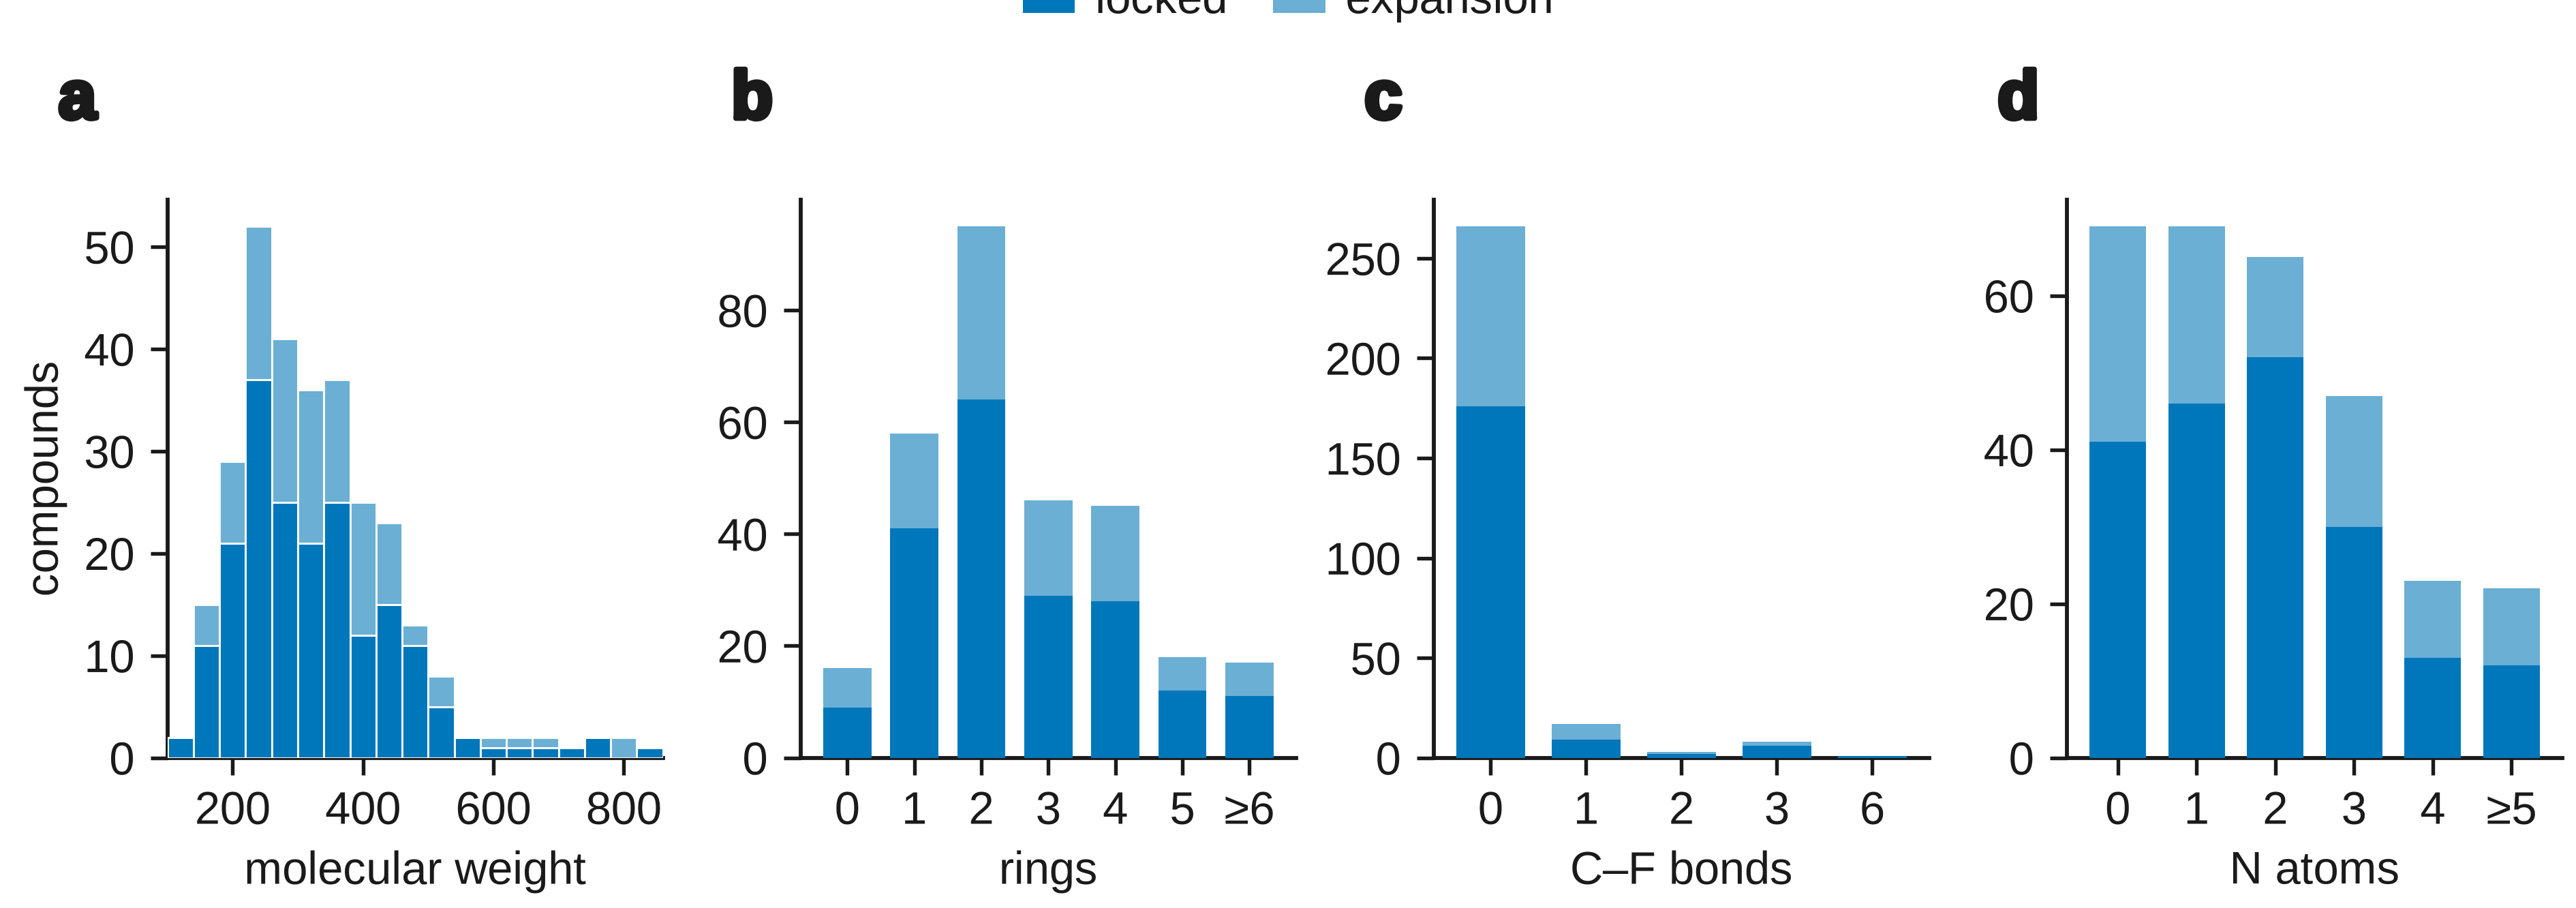
\includegraphics[width=0.92\linewidth]{fig_chemspace.png}
  \caption{Pooled headline chemistry ($n{=}300$; panels on validate-clean $n{=}295$).
  (a)~MW (median 306). (b)~RDKit rings (median 2). (c)~C--F bonds. (d)~N atoms.
  Stacked: locked (dark) vs expansion (light). Mid-size literature space, not a NIST toy set.}
  \label{fig:fig-chemspace}
\end{figure}

\subsection{Difficulty, balance, and scoring contract}

\textbf{Difficulty} is declared \emph{a priori} by RDKit ring analysis: \emph{simple} iff
$\leq$2 rings, no fused/spiro/bridgehead system, $\leq$22 heavy atoms; else \emph{complex}
(151/149 on $n{=}300$).
The released benchmark is \textbf{50/50 by design}; the eligible corpus is 17.5\% simple /
82.5\% complex.
Reweighted to corpus composition on the validate-clean subset, top-1 falls 39.3\% $\to$
\textbf{26.5\%} [21--32] and recall 44.1\% $\to$ \textbf{31.3\%} [25--37]
(Appendix~\ref{app:extended}).
We report both: the reweighted figure is the better estimate for an arbitrary paper, and the
50/50 figure is the comparable leaderboard number (Table~\ref{tab:headline}).

\textbf{Scoring.} A prediction is correct if RDKit InChIKey \textbf{connectivity} (first 14
characters) matches --- we score \emph{constitution}.
Full stereo-sensitive InChIKey is reported on the validate-clean subset
(Appendix~\ref{app:extended}).
External submissions: up to three ranked SMILES per \texttt{qid}, no structure hints
(\texttt{docs/LEADERBOARD.md}; \texttt{scripts/score\_submission.py}).
Primary metrics (report all three): \textbf{top-1} (best-ranked candidate matches at
connectivity); \textbf{generation recall} (reference in the pool \emph{before} re-ranking);
\textbf{verification precision $|$ recall} (correct top-1 among recall-positive compounds).
Confidence intervals are bootstrap 95\%; paired model differences use McNemar with Holm correction.

\section{Experimental setup}
\label{sec:setup}

\paragraph{Blind payload and solver.}
The solver sees four JSON fields per \texttt{qid}: \texttt{formula} (as from HRMS),
\texttt{ir\_bands\_cm-1}, \texttt{h\_nmr}, \texttt{c\_nmr} --- peak lists as printed
(Figure~\ref{lst:payload}).
No name, SMILES, scaffold, atom-type hint, or retrieved spectrum; ground truth is scored
offline.
Frontier LLM agent (Claude Opus via consumer subscription), closed-book, one sub-agent per
batch, RDKit formula check only.
No fine-tuning, no paid API, \textbf{no thinking tier} for the core protocol.
Inference is \textbf{not} exactly reproducible (no pinned snapshot, temperature or seed ---
Section~\ref{sec:limitations}).
\textbf{Scoring is reproducible}: frozen predictions, ground truth and scorers regenerate every
training-free number.

\begin{figure}[ht]
\centering
\begin{minipage}{0.98\linewidth}
\begin{framed}
\noindent
\begin{minipage}[c]{0.56\linewidth}
\begin{lstlisting}[style=benchjson]
{
  "qid": "v3-R25",
  "formula": "C10H14N2O",
  "ir_bands_cm-1": [1679, "..."],
  "h_nmr": "[printed 1H list]",
  "c_nmr": "[printed 13C list]"
}
\end{lstlisting}
\end{minipage}\hfill
\begin{minipage}[c]{0.40\linewidth}
\centering
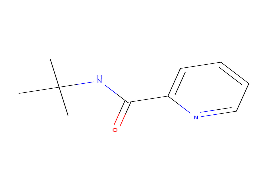
\includegraphics[width=\linewidth]{fig_listing_mol.pdf}\\[0.2em]
{\scriptsize\itshape gold held out}\\[-0.1em]
{\scriptsize 2-pyridyl picolinamide}
\end{minipage}
\end{framed}
\end{minipage}
\caption{\textbf{Listing 1.} Solver-facing payload (abridged), IRexp
JSON$+$molecule layout. Gold constitution (right) is held out.
Only disclosed fragments are shown (v3-R25 / C$_{10}$H$_{14}$N$_{2}$O / IR 1679);
full lists ship with the bench. Source: IRexp~\citep{yabbarov2026irexp};
this PDF is not a Data Descriptor.}
\label{lst:payload}
\end{figure}

\paragraph{Scoring contract and candidate budget.}
A deposit is JSONL of \texttt{\{qid, candidates: [SMILES,\ldots]\}} under a stated budget.
The scorer reports the three Section~\ref{sec:benchmark} metrics at InChIKey-connectivity,
with bootstrap 95\% CIs.
Self-ranking vs forward-verified re-ranking must be labelled; they are not interchangeable.
Headline protocol: $\leq$3 ranked SMILES per \texttt{qid}.
On the 60-compound arm Claude returned mean 2.20 candidates vs 3.00 for the other vendors
(recall rankings approximate).
\textbf{Generate-wide} (that arm only): ten independent solvers $\times$ up to six SMILES,
pooled then re-ranked --- not the $n{=}300$ reporting budget.

\paragraph{Forward-verification, expansion, and probes.}
Generate $\to$ forward-predict $^{13}$C (blind to the observed list) $\to$ re-rank by
symmetric chamfer on $^{13}$C peak sets (Section~\ref{sec:forward-verify}); instrumented on
the locked $n{=}194$ only.
Expansion is a pre-registered 106-compound draw from the same \texttt{irexp\_resolved}
sampler after the $n{=}194$ lock, with the same $^{13}$C-overread audit
(Section~\ref{sec:expansion}): five flags stay in the $n{=}300$ headline; validate-clean
$n{=}295$ is appendix; expansion-106 forward-verify was not run.
A later 230-compound draw toward $n{\approx}500$ is deposited and unscored
(Section~\ref{sec:expansion}).
Controls: formula-only / recency (Section~\ref{sec:contamination}); four-vendor replication
on a 60-compound arm (Section~\ref{sec:cross-vendor}); generate-wide sampling; HOSE lookup
and GNN $^{13}$C verifiers; small IRexp-fine-tuned generator probe (excluded from headline
claims).

\section{Results}
\label{sec:results}

\subsection{Headline performance}
\label{sec:headline}

\begin{table}[ht]
\caption{Headline elucidation ($n{=}300{=}194$ locked $+$ $106$ expansion).
Bootstrap 95\% CIs; validate-clean $n{=}295$ in Appendix~\ref{app:extended}.}
\label{tab:headline}
\centering
\small
\begin{tabular}{@{}lr@{}}
\toprule
metric & $n{=}300$ \\
\midrule
top-1 exact constitution & \textbf{39.3\%} (118/300) [34--45] \\
\quad simple ($n{=}151$) & 58.3\% (88/151) \\
\quad complex ($n{=}149$) & 20.1\% (30/149) \\
generation recall (top-3) & \textbf{44.3\%} (133/300) [39--50] \\
\bottomrule
\end{tabular}
\end{table}

On the validate-clean subset, scaffold-level recovery is 64\% (simple 80\%, complex 48\%) and
mean best Tanimoto is 0.66; accuracy falls with size (67.9\% top-1 at $\leq$15 heavy atoms,
42.8\% at 16--25, 16.7\% above 25; $n{=}53/152/90$; Appendix~\ref{app:extended}).
On the locked 194, of 137 analysable top-1 misses, \textbf{76.6\%} are constitutional isomers of the true
structure; only \textbf{22.6\%} share the true Murcko scaffold --- wrong connectivity at the
right composition, not mostly fine regiochemistry (not re-run on the expansion).
A 24-compound four-model Claude comparison is capability-sensitive (Haiku $\subset$ Sonnet
$\subset$ Opus $\subset$ Fable) but underpowered for adjacent ranks, with a disclosed protocol
asymmetry (Section~\ref{sec:limitations}); a battery-electrolyte subset ($n{=}46$) matches the
locked-slice regime (26\% top-1; recall-bound).

\begin{table}[ht]
\caption{Generation by slice. Headline is pooled $n{=}300$, not locked 194 alone.}
\label{tab:slices}
\centering
\small
\begin{tabular}{@{}lrrr@{}}
\toprule
 & locked ($n{=}194$) & expansion ($n{=}106$) & pooled ($n{=}300$) \\
\midrule
top-1 & 55/194 (28.4\%) & 63/106 (59.4\%) & \textbf{118/300 (39.3\%)} \\
generation recall & 65/194 (33.5\%) & 68/106 (64.2\%) & \textbf{133/300 (44.3\%)} \\
\bottomrule
\end{tabular}
\end{table}

The expansion slice is easier for this solver than the locked 194 (59.4\% vs 28.4\% top-1);
pooling does not hide that gap.
Self-ranking precision $|$ recall on the pooled generation cohort is 118/133 (88.7\%) ---
that is \emph{not} forward-verification precision (Section~\ref{sec:forward-verify}).

\subsection{Is the model reading the spectra?}
\label{sec:contamination}

\begin{table}[ht]
\caption{Formula-only control (paired, $n{=}60$).}
\label{tab:formula-only}
\centering
\small
\begin{tabular}{@{}lrr@{}}
\toprule
condition & top-1 & recovered (top-3) \\
\midrule
formula only & \textbf{3/60 (5\%)} & 3/60 (5\%) \\
formula + IR + $^1$H + $^{13}$C & 14/60 (23\%) & 19/60 (32\%) \\
\bottomrule
\end{tabular}
\end{table}

Outcomes are perfectly nested (McNemar $p{=}0.001$).
Accuracy is flat in source-paper year across the locked 194 ($r{=}{-}0.007$), bounding pretraining
recall of specific papers.
We claim a \textbf{strong bound, not exclusion} of contamination
(Section~\ref{sec:limitations}).

\begin{figure}[ht]
  \centering
  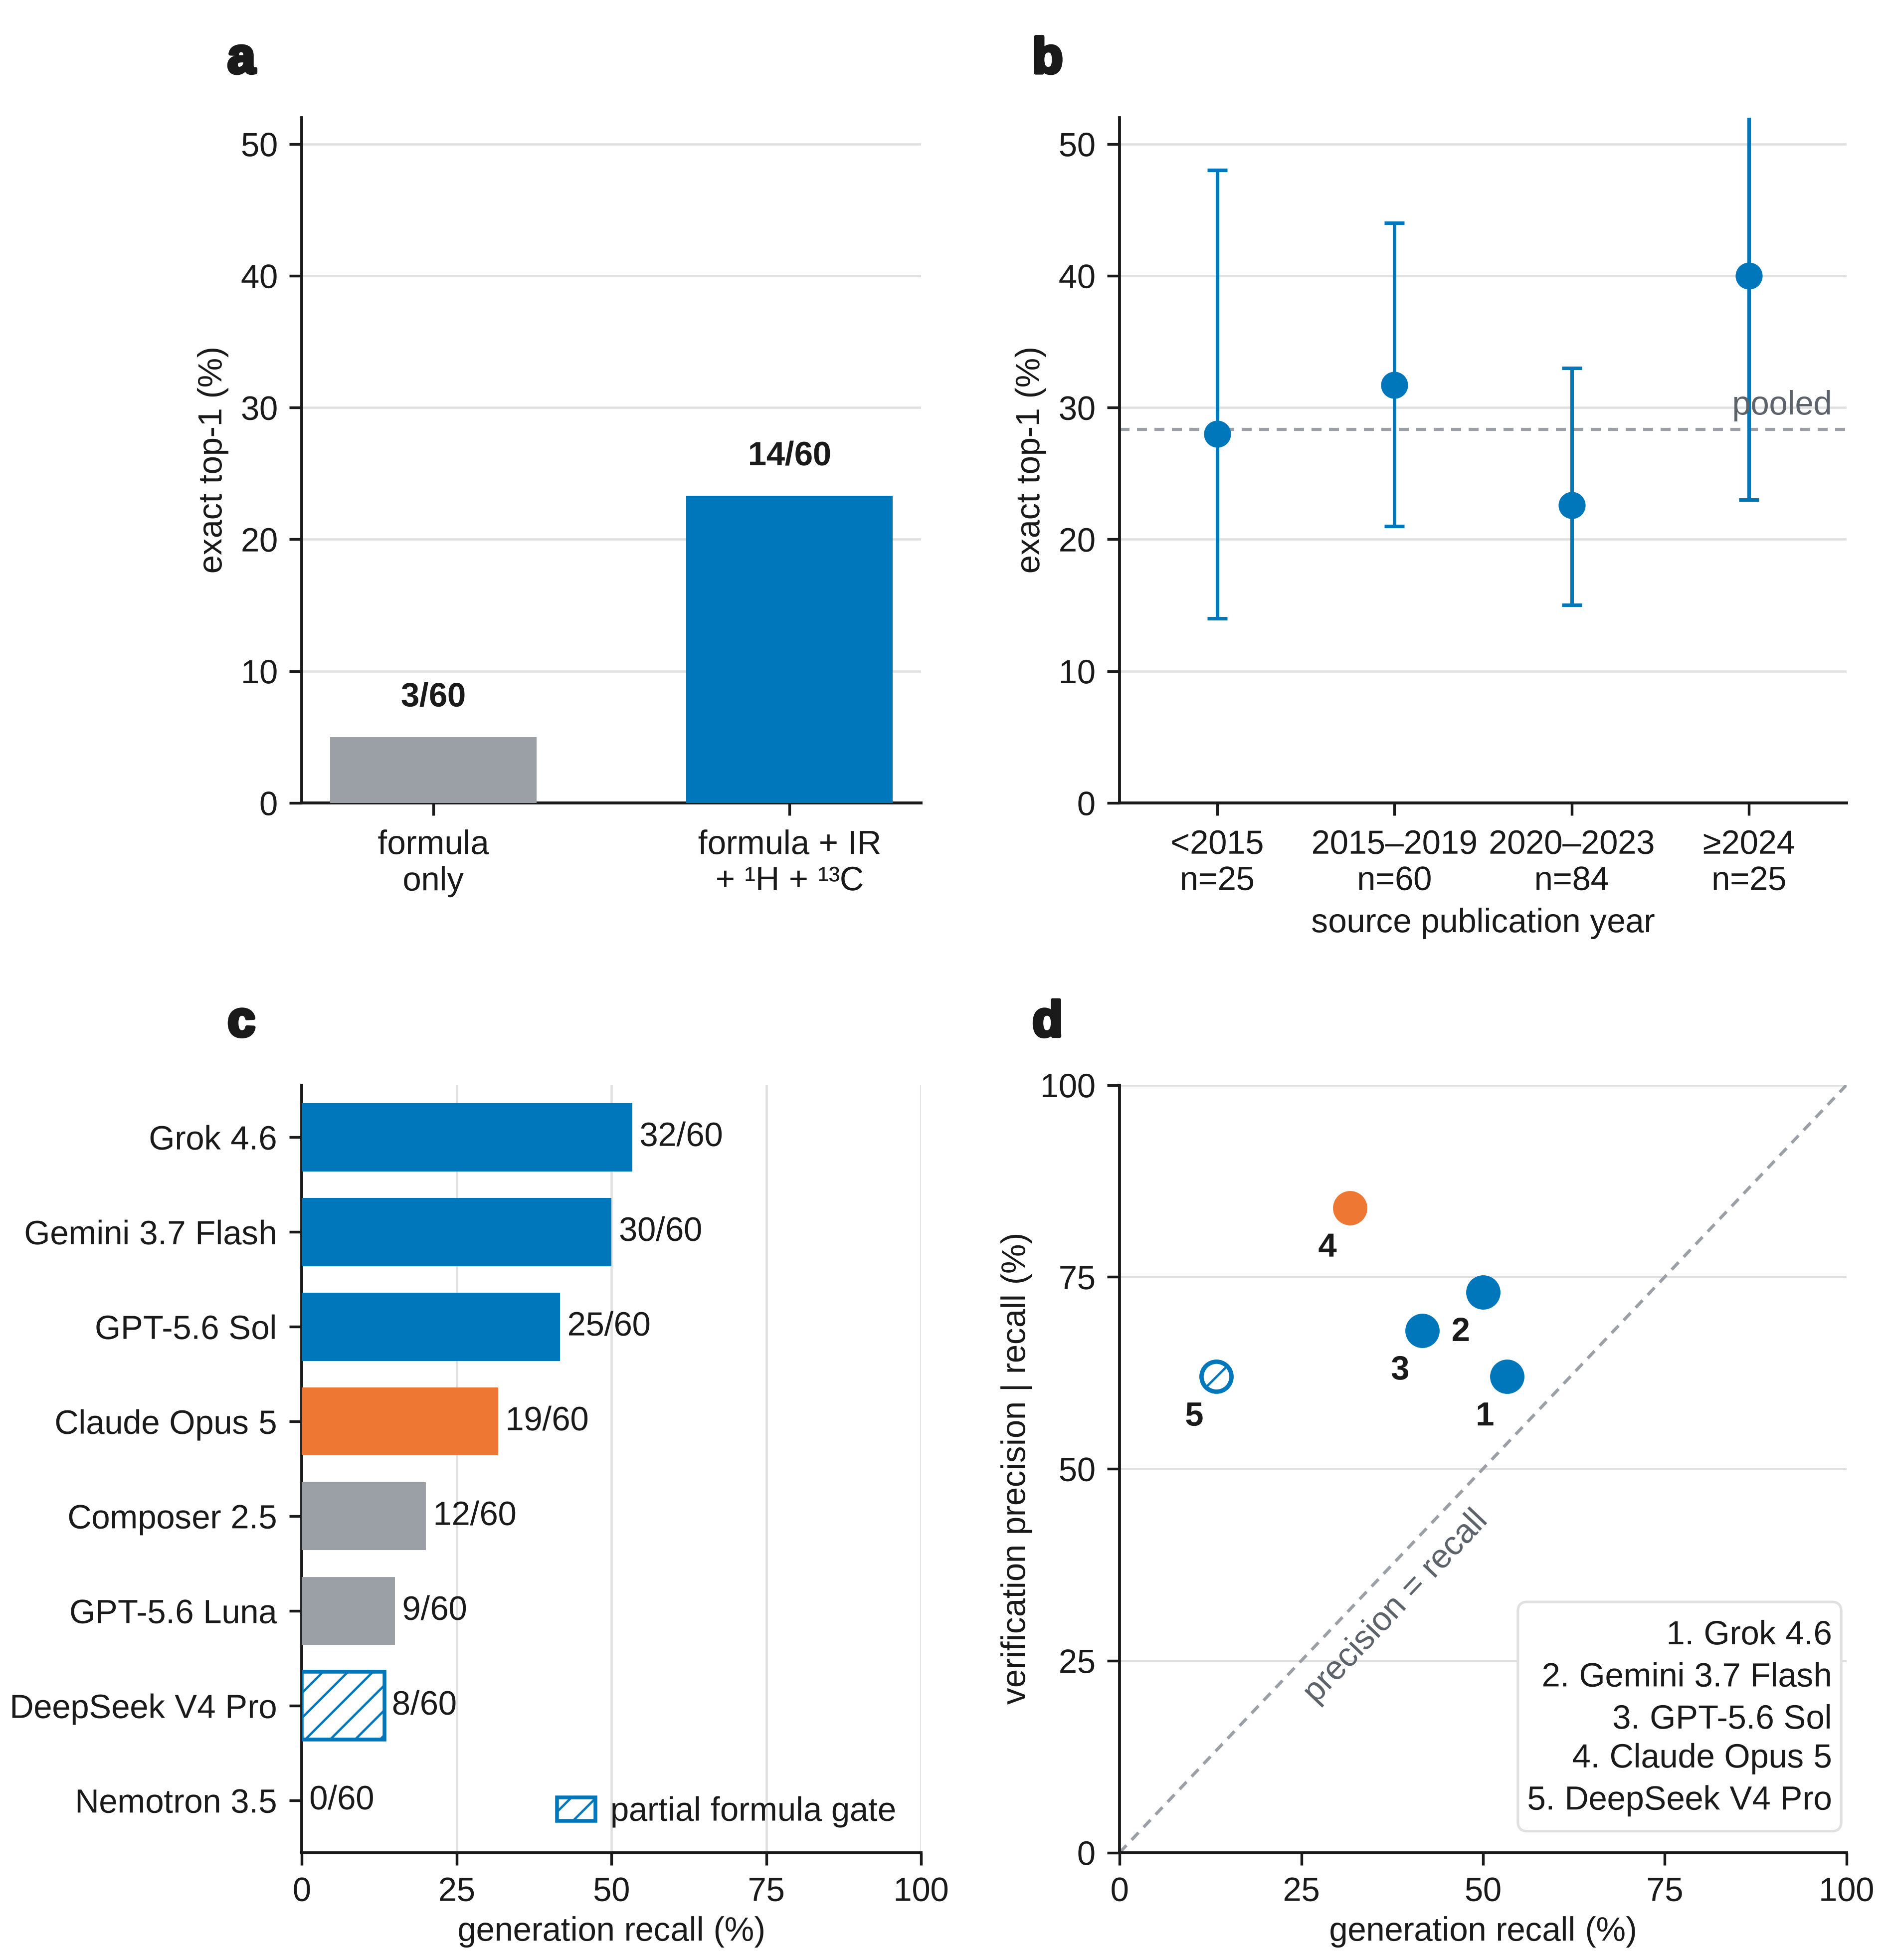
\includegraphics[width=0.62\linewidth]{fig_robustness.png}
  \caption{Robustness on instrumented arms (formula-only / cross-vendor $n{=}60$;
  recency $n{=}194$): formula-only collapse, flat recency, four-vendor recall $\ll$ precision.}
  \label{fig:fig-robustness}
\end{figure}

\subsection{Cross-vendor replication}
\label{sec:cross-vendor}

Grok 4.6, Gemini 3.7 Flash and GPT-5.6 Sol solved the same 60-compound arm under the
identical protocol.
\textbf{Verification precision exceeds generation recall in every arm}; bootstrapping
separates the paired gap for Claude (+52.5 points), GPT-5.6 Sol (+26.3) and Gemini (+23.3);
Grok's gap (+9.2) is directional.

\begin{table}[ht]
\caption{Cross-vendor decomposition ($n{=}60$). Recall and precision use different denominators.}
\label{tab:cross-vendor}
\centering
\small
\begin{tabular}{@{}lrrr@{}}
\toprule
model & generation recall & verification precision $|$ recall & multi-candidate only \\
\midrule
Claude Opus & 19/60 = 32\% & 16/19 = 84\% & 10/13 = 77\% \\
Grok 4.6 & 32/60 = 53\% & 20/32 = 62\% & 20/32 = 62\% \\
Gemini 3.7 Flash & 30/60 = 50\% & 22/30 = 73\% & 22/30 = 73\% \\
GPT-5.6 Sol & 25/60 = 42\% & 17/25 = 68\% & 16/24 = 67\% \\
\bottomrule
\end{tabular}
\end{table}

Candidate budgets differ (Claude mean 2.20 vs others 3.00), so recall rankings are
approximate.
A clean-clone control for Grok bounds key leakage (McNemar $p{=}0.39$).

\subsection{Forward-verification decomposition}
\label{sec:forward-verify}

\begin{figure}[ht]
  \centering
  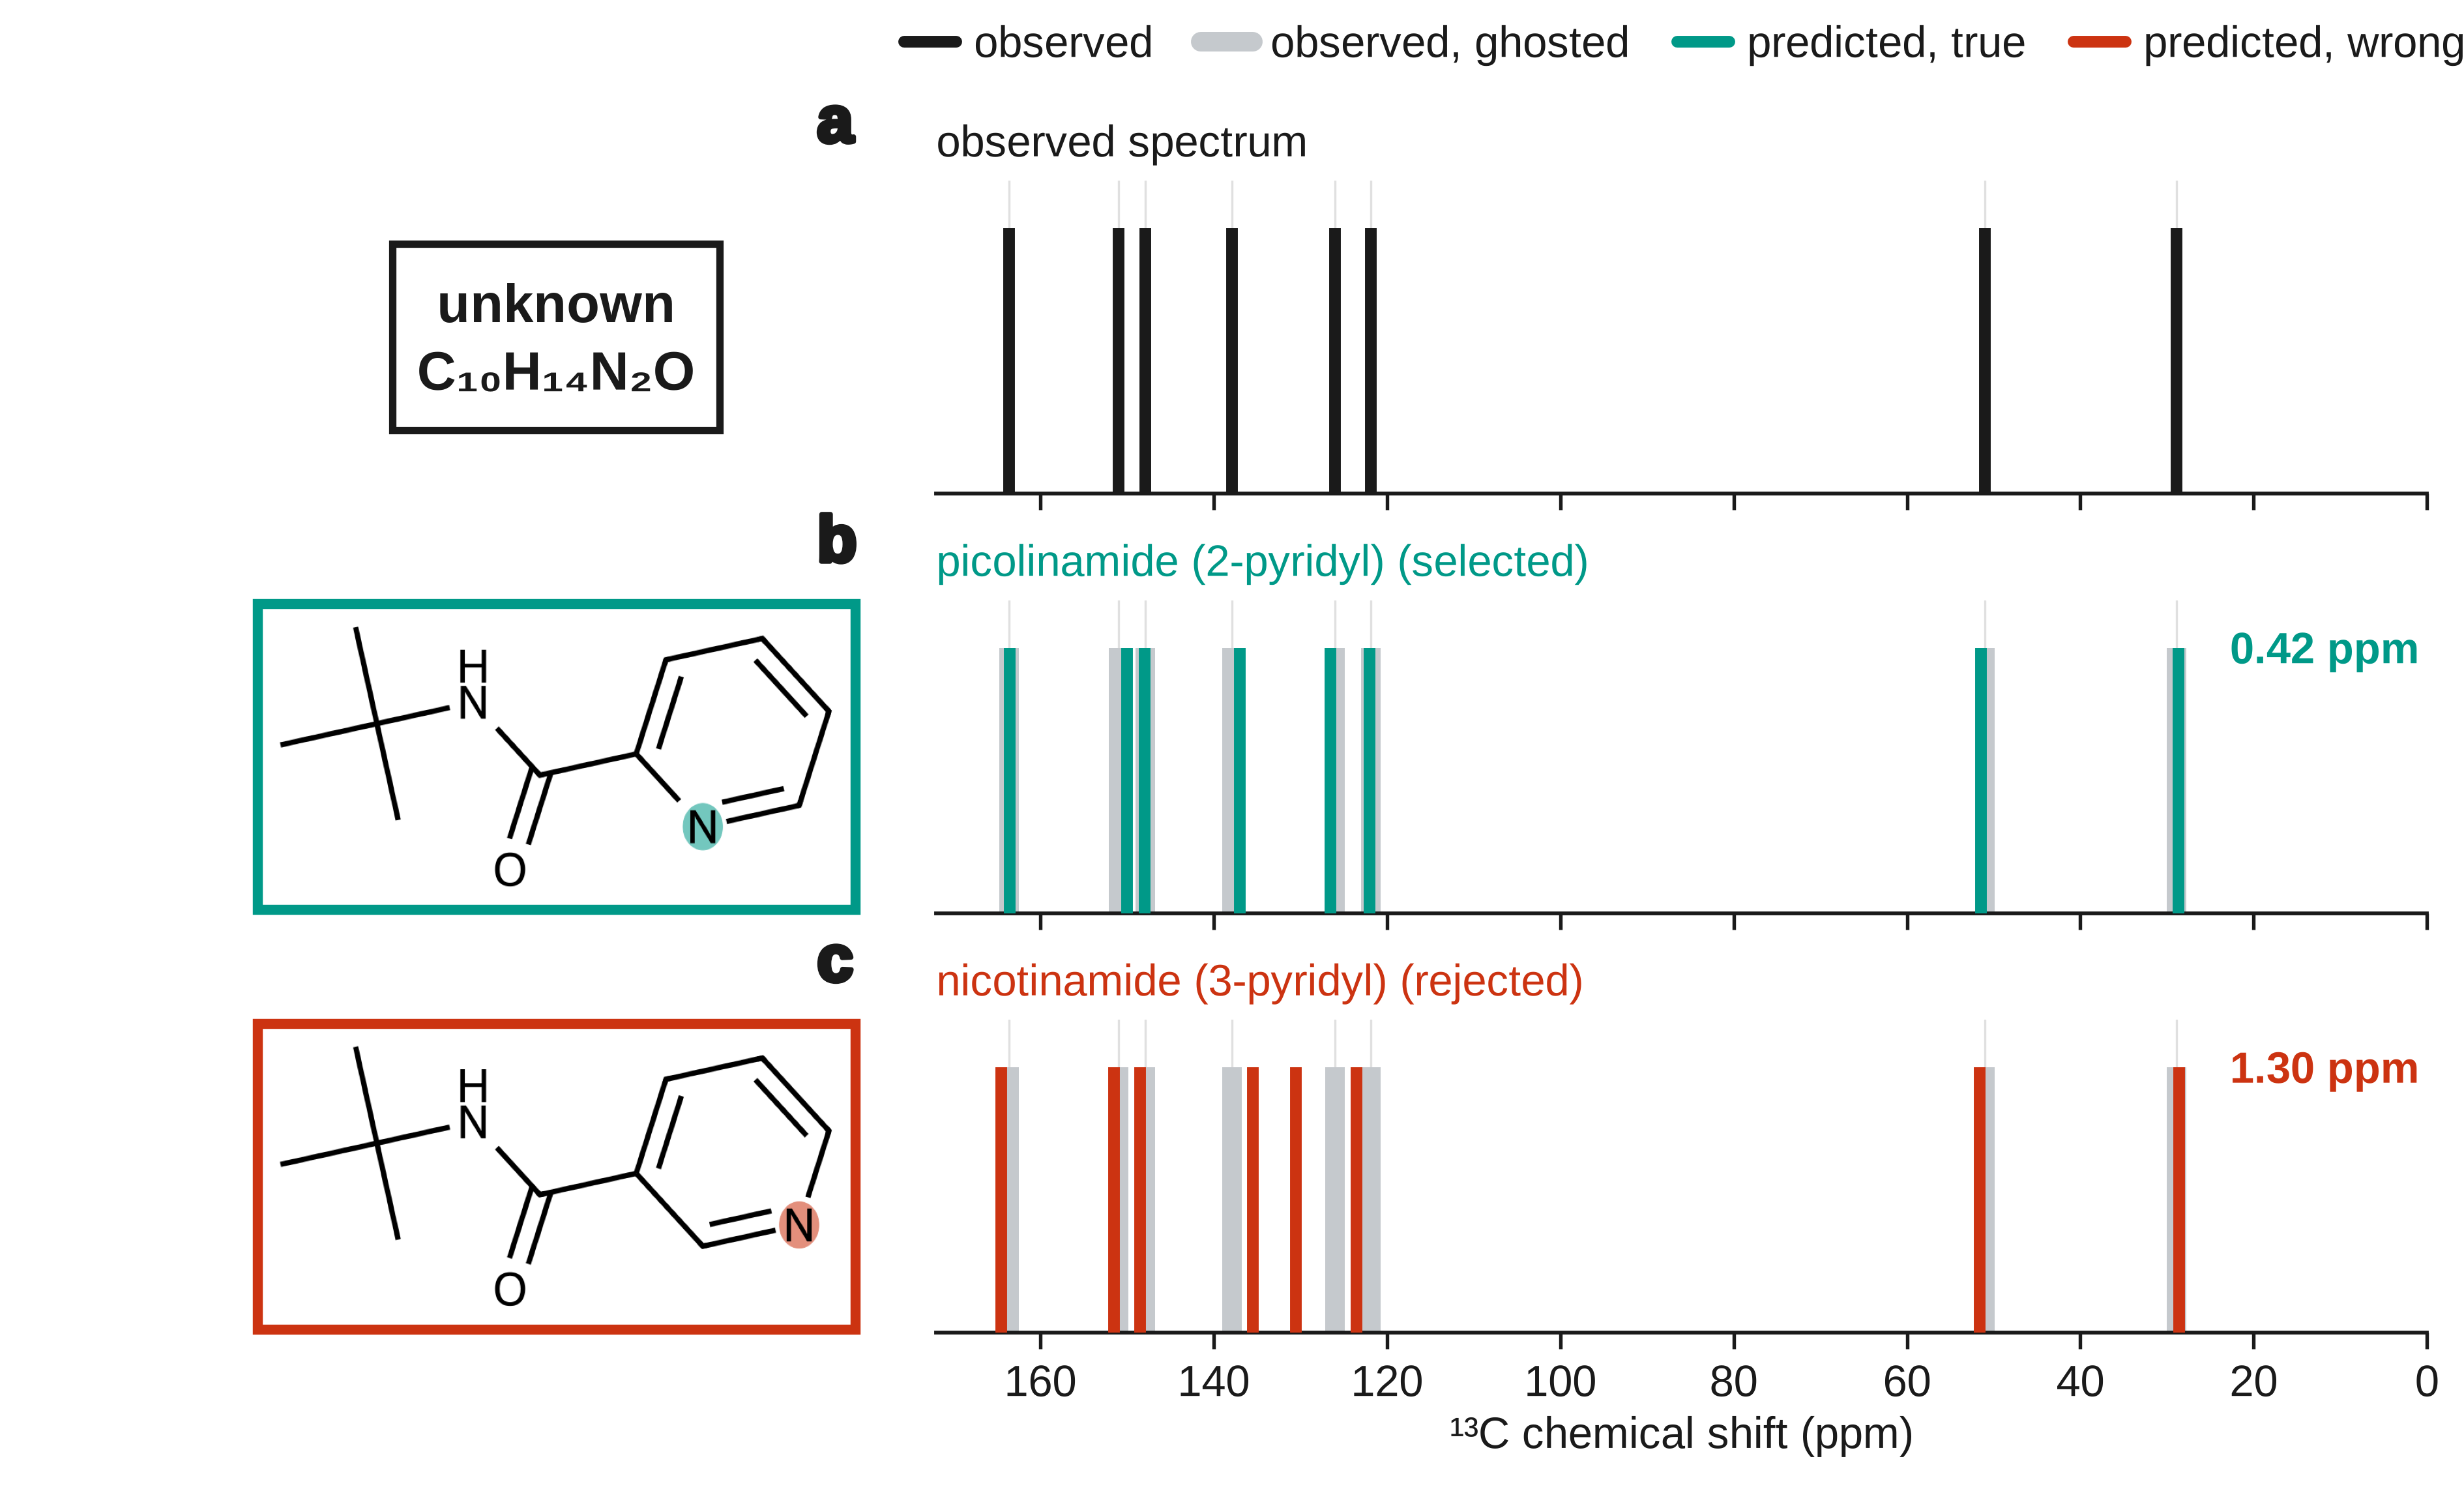
\includegraphics[width=0.72\linewidth]{fig_mechanism.png}
  \caption{Locked v3-R25: self-rank prefers 3-pyridyl; forward $^{13}$C recovers 2-pyridyl
  (chamfer 0.42 vs 1.30~ppm) --- a verify-save, not a recall win (Table~\ref{tab:cases}).}
  \label{fig:fig-mechanism}
\end{figure}

\begin{table}[ht]
\caption{Forward-verify on the instrumented slice ($n{=}194$).
Pooled $n{=}300$ in Table~\ref{tab:headline} is generation only.}
\label{tab:fverify}
\centering
\small
\begin{tabular}{@{}lrr@{}}
\toprule
 & 60-compound arm & locked slice ($n{=}194$) \\
\midrule
generation recall & 19/60 (32\%) & 65/194 (34\%) \\
top-1, solver self-ranking & 14/60 (23\%) & 55/194 (28\%) \\
top-1, forward-verified re-ranking & 16/60 (27\%) & 58/194 (30\%) \\
precision $|$ recall --- forward-verification & 16/19 (84\%) & 58/65 (\textbf{89\%}) \\
multi-candidate only --- forward-verification & 10/13 (77\%) & 30/37 (81\%) \\
\bottomrule
\end{tabular}
\end{table}

When the true structure is among the candidates, forward-verification selects it in 58/65
cases (89\%).
Where a choice existed ($n{=}37$), forward-verification is correct on 30/37 (81\%) against a
54.0\% derangement floor (+27.1 points).
The margin over self-ranking is \textbf{small and unresolved} (seven gained, four lost;
McNemar $p{=}0.55$) --- we do \textbf{not} claim an accuracy advance.
Precision is high while recall binds: no re-ranking repairs the 129/194 compounds on this
slice where the true structure was never proposed (Figure~\ref{fig:fig1}c;
diagnostic repeat in Figure~\ref{fig:fig-wall}).

\paragraph{Worked cases.}
Three locked-slice deposits instantiate the wall (Appendix Table~\ref{tab:cases}; expansion
qids reuse R22/R25 --- IDs below are locked-round labels).
\textbf{main-R06} (C$_{29}$H$_{30}$FNO$_{2}$): true acridinedione never enters the 3-candidate
pool (Tanimoto-0.90 regioisomer); verifier unused.
\textbf{v3-R25} (C$_{10}$H$_{14}$N$_{2}$O): verify-save --- self-rank prefers 3-pyridyl,
forward $^{13}$C recovers 2-pyridyl (chamfer 0.42 vs 1.30~ppm; Figure~\ref{fig:fig-mechanism}).
\textbf{v3-R26} (C$_{14}$H$_{11}$N$_{3}$O$_{3}$): verify-fail --- true 3-nitrophenyl isomer in
the pool but 2-nitro ranked first (chamfer 1.35 vs 1.36~ppm).

\paragraph{Generate-wide.}
Ten solver agents, up to six candidates each, pooled and re-ranked on the 60-compound arm:
recall 32\% $\to$ \textbf{42\%}, top-1 23\% $\to$ \textbf{30\%} (McNemar $p{=}0.34$);
verification precision falls 84\% $\to$ 72\%.
The training-free ceiling remains recall-limited.

\begin{figure}[ht]
  \centering
  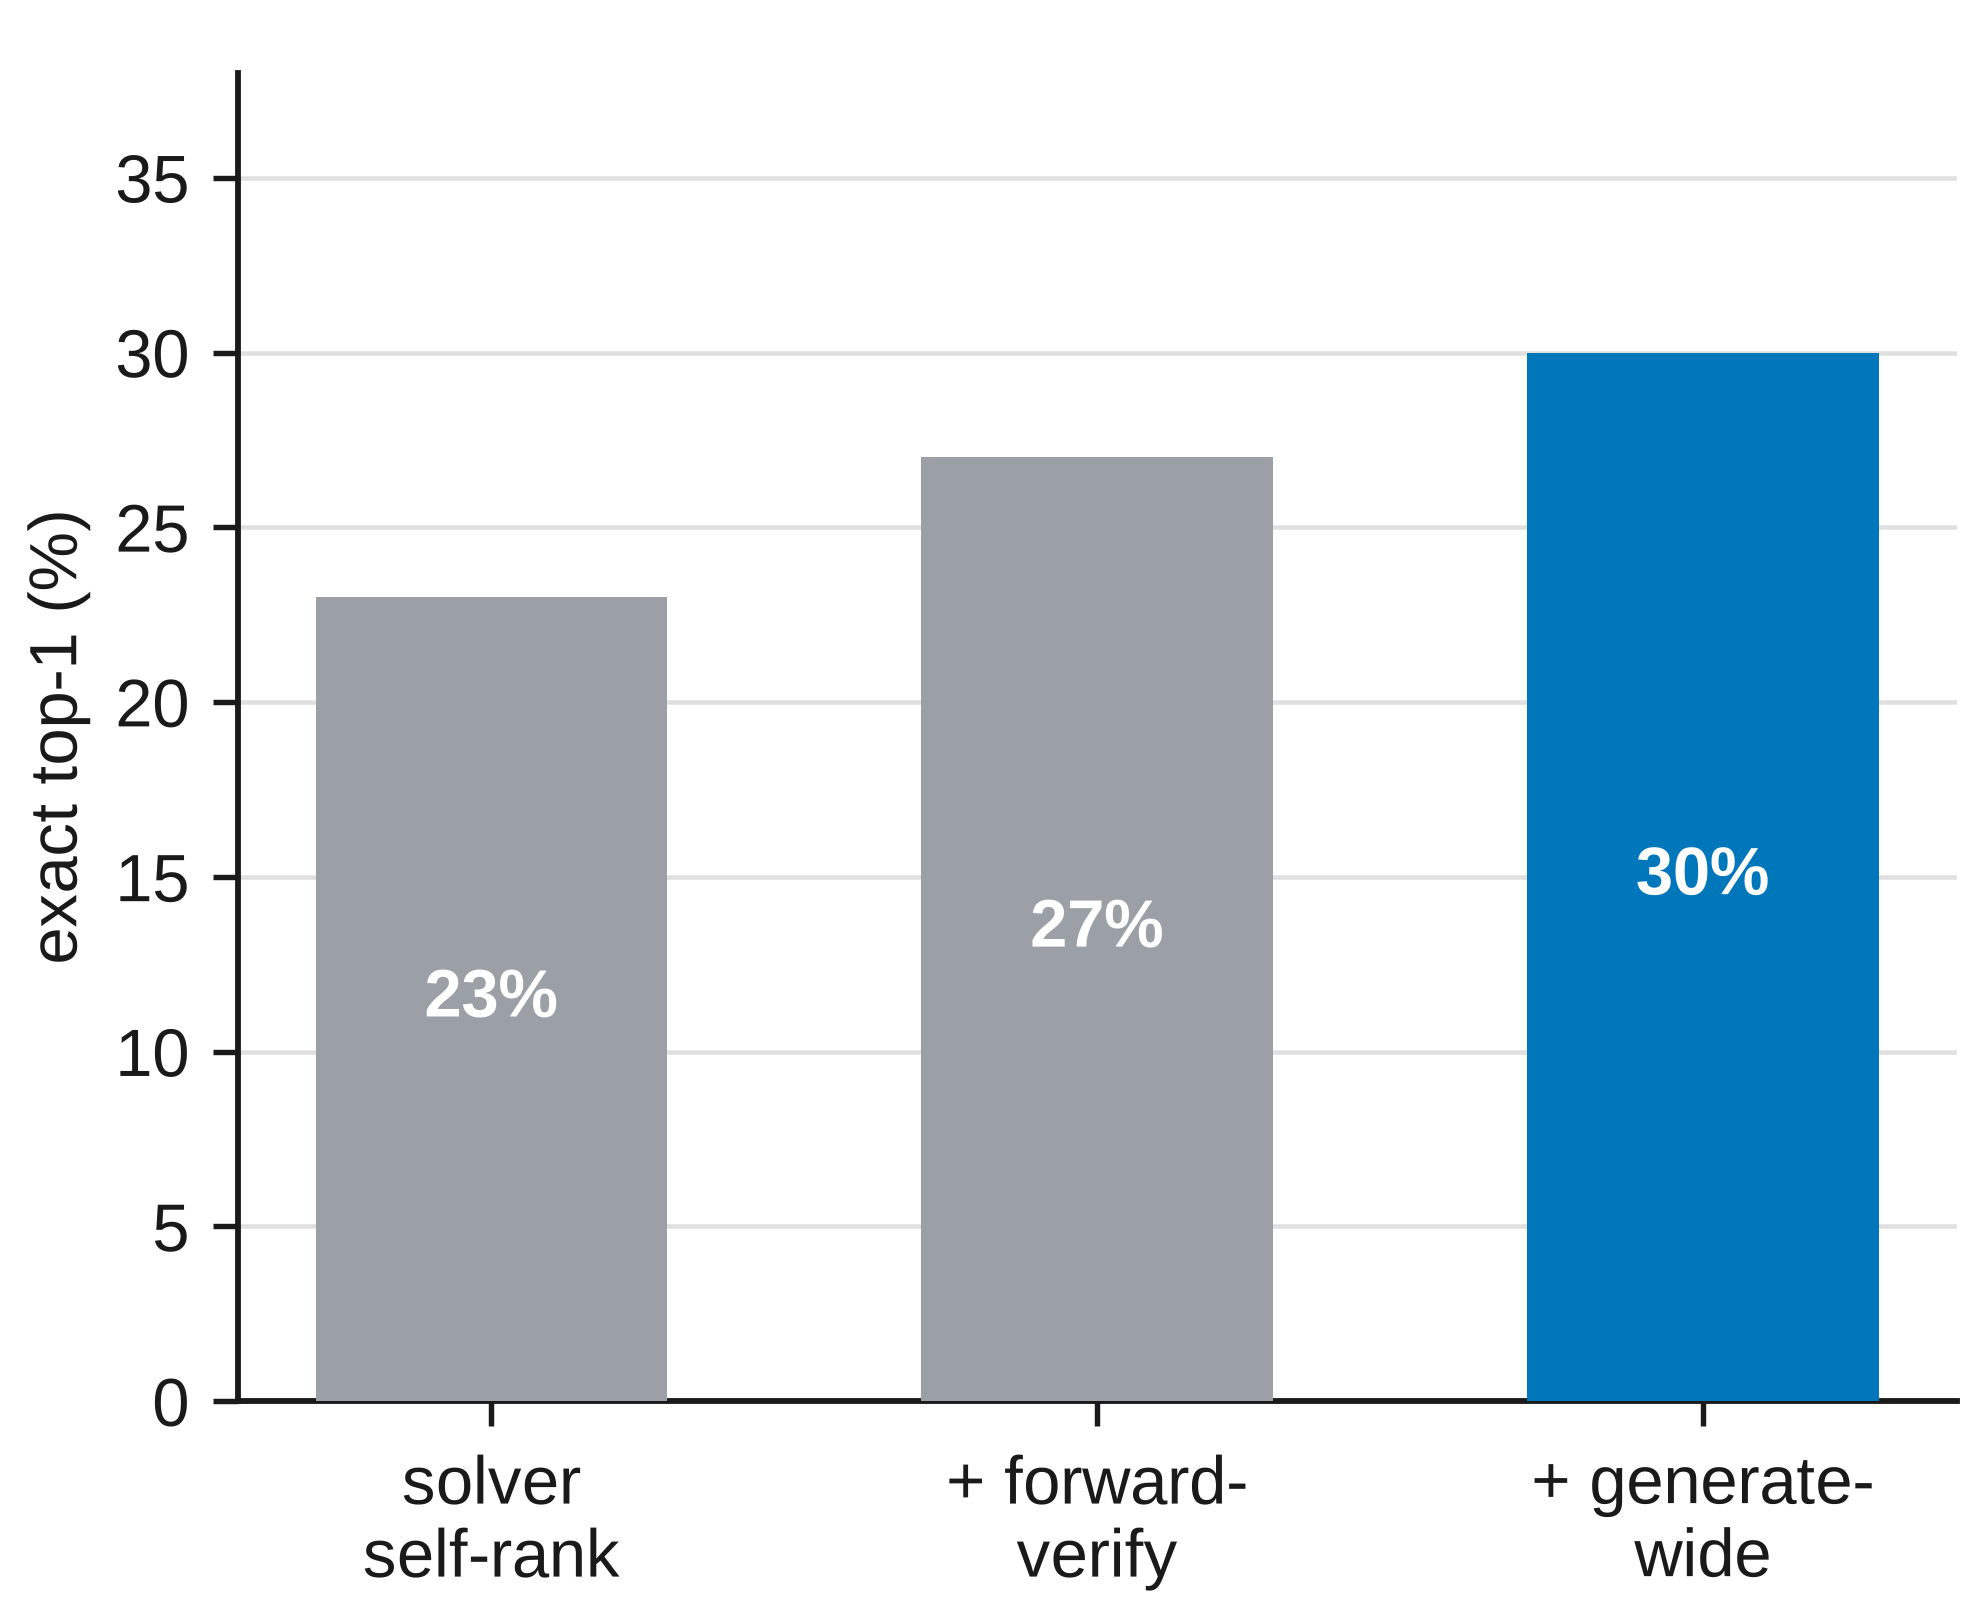
\includegraphics[width=0.52\linewidth]{fig3_method.png}
  \caption{Inference ladder on the 60-compound arm: 23\% $\to$ 27\% $\to$ 30\% top-1.
  Generate-wide lifts recall (32\% $\to$ 42\%); the wall is proposal, not ranking.}
  \label{fig:fig3-method}
\end{figure}

\paragraph{Non-LLM verifiers.}
On the same candidate sets, a HOSE-style lookup ties self-ranking; a modest GNN reaches
59/65 (91\%) vs the LLM verifier's 58/65 (89\%) --- directional.
Deranging observed $^{13}$C pairings collapses precision ($p{=}0.001$).
A small IRexp-fine-tuned generator pooled with Claude lifts locked-slice recall 33.5\% $\to$ 54.1\% and
top-1 28.4\% $\to$ 35.1\% (McNemar $p{=}0.015$), showing the wall is a property of
\textbf{training-free elicitation}, not of the task.

\subsection{Decomposition across published literature}
\label{sec:literature}

Any system reporting top-1 $= a$ and top-$k = b$ implies recall $\geq b$ and conditional
precision $\leq a/b$.
Applying this to published figures (\texttt{scripts/literature\_decomposition.py}):

\begin{table}[ht]
\caption{Selected literature decomposition rows (connectivity-scored or as published).}
\label{tab:lit-decomp}
\centering
\scriptsize
\setlength{\tabcolsep}{3pt}
\begin{tabular}{@{}p{2.6cm}p{2.4cm}rrrr@{}}
\toprule
system & data ($n$) & top-1 & top-$k$ ($k$) & recall & prec. \\
\midrule
this work, solver alone & literature (300) & 39.3\% & 44.3\% (3) & 44.3\% & 88.7\% \\
this work + forward-verify & literature (194) & 29.9\% & 33.5\% (3) & 33.5\% & \textbf{89.2\%} \\
NMR-Solver~\citep{jin2025nmrsolver} & literature (450) & 52.9\% & 67.3\% (10) & $\geq$67.3\% & $\leq$78.6\% \\
NMRAgent~\citep{fang2026nmragent} & literature (450) & 61.6\% & 70.0\% (10) & $\geq$70.0\% & $\leq$88.0\% \\
Espejo Morales~\citep{espejo2026agentic} & education (236) & 80.9\% & 90.0\% (5) & $\geq$90.0\% & $\leq$89.9\% \\
Espejo Morales~\citep{espejo2026agentic} & industrial (34) & 20.6\% & 29.1\% (5) & $\geq$29.1\% & $\leq$70.9\% \\
Alberts, 6--13 atoms~\citep{alberts2025benchmarks} & NIST IR (3,455) & 63.8\% & 84.0\% (10) & 84.0\% & 75.9\% \\
SpecX, scaffold split~\citep{xiang2026specx} & simulated (99,439) & 29.7\% & 50.6\% (10) & 50.6\% & 58.7\% \\
\bottomrule
\end{tabular}
\end{table}

\textbf{Three groups changed only the data}, and recall carried \textbf{68\%} (NMR-Solver
simulated $\to$ real), \textbf{70\%} (SpecX random $\to$ scaffold) and \textbf{83\%}
(Espejo education $\to$ industrial) of each collapse.
Recall binds where spectra are real and heterogeneous; ranking dominates on simulated or
single-library data.
The solver-alone precision column on $n{=}300$ is self-ranking (118/133); the
forward-verify row is the instrumented $n{=}194$ slice (58/65) --- not interchangeable.

\subsection{Pre-registered expansion, pooled headline, and scale roadmap}
\label{sec:expansion}

The $n{=}300$ headline is the pre-registered pool of the locked 194 and a 106-compound
expansion draw (Table~\ref{tab:slices}; Appendix Tables~\ref{tab:expansion},~\ref{tab:clean295}).
Five $^{13}$C-overread flags (R12, R22, R25, R82, R91) stay in the 300; validate-clean is
116/295 (39.3\%) top-1 / 130/295 (44.1\%) recall.
The expansion slice is easier (59.4\% vs 28.4\% top-1) --- disclosed, not hidden.
A Fable arm is incomplete (68/106; not scored; never pooled).
Figure~\ref{fig:fig-wall} and Table~\ref{tab:fverify} remain the $n{=}194$ instrumented
forward-verified diagnosis; expansion-106 fverify was \textbf{not} run.

\paragraph{Scale roadmap / larger blind round.}
A second pre-registered draw toward $n{\approx}500$ (230 compounds; 115/115 simple/complex;
six $^{13}$C-overread flags known \emph{before} any solve) now has \textbf{230/230} Opus
deposits and a frozen 690-candidate file.
Scoring is \textbf{deferred}: the answer key is withheld, no top-1 or recall exists, and
forward-verify was not run on this round.
Those deposits used a thinking-tier consumer arm and are not interchangeable with the
no-thinking $n{=}300$ protocol until scored under a declared contract.
This round is \textbf{not} pooled into the headline and is not a wall figure.

\section{Discussion}
\label{sec:discussion}

Frontier LLMs are \textbf{good verifiers} ($\approx$89\% conditional precision on the
$n{=}194$ instrumented slice) and \textbf{weak proposers} (44\% generation recall on
$n{=}300$; 34\% on the instrumented 194) on real literature peak lists --- propose $\gg$
verify, not the reverse.
The primary research contribution is the \textbf{benchmark + stage decomposition +
contamination/cross-vendor diagnosis}, not a solved elucidator and not a Data Descriptor
for IRexp.
The expansion slice scored higher than the locked 194 (Section~\ref{sec:expansion}); pooling
does not erase that gap.
The $n{\approx}500$ deposits do not yet change any scored number.

\paragraph{Reporting contract.}
External work on IRSpectra-Bench should deposit ranked SMILES under the released protocol and
report, at minimum: (i) top-1 constitution, (ii) generation recall, (iii) verification
precision $|$ recall, with bootstrap CIs and candidate budget.
Top-1 alone conflates the two stages.
Nonsignificant ladder gains (forward-verification vs self-ranking, $p{=}0.55$; generate-wide
top-1, $p{=}0.34$) should be cited as \textbf{diagnostic}, not as accuracy advances.
Corpus-reweighted top-1 (\textbf{26.5\%} on the validate-clean subset) is the better estimate
for an arbitrary literature draw.
Training is not foreclosed: IRexp fine-tuning lifts recall to 54\%.
Those gains compound with open experimental data, honest benchmarks, and inference scaffolding that
transfers to each new model.

\subsection{Implications for agentic elucidation}
\label{sec:agentic}

The diagnosis implies an \textbf{asymmetric pipeline}, not another verifier stacked on a thin
pool.
Proposal is the expensive stage: diversity, tool-use into enumeration / database search /
formula-constrained decode, or generate-wide sampling that actually enlarges the pool.
Verification is cheap: once the true constitution is proposed, training-free
forward-verification selects it $\approx$89\% of the time on the instrumented $n{=}194$
slice (58/65).
Spending the budget on a second ranker cannot recover the 129/194 compounds that were never
proposed.

IR-Agent-style table-interpretation and retrieve tools~\citep{noh2025iragent} are complementary
\emph{feature} agents --- they improve how a spectrum is read and how a given pool is
re-ranked.
MolQuest- and Espejo-style architecture search~\citep{han2026molquest,espejo2026agentic}
still needs this stage contract: a better reader that does not change
$P(\text{true}\in\text{pool})$ cannot move top-1 on a recall-bound bench.
The next ICLR-relevant agent is a \textbf{proposer}, not a second verifier:
formula-constrained generators, fragment assembly, and search that change that probability.
We are \textbf{not} shipping another ChemCrow-for-IR or a SpectraLLM-style fine-tune:
the bench is a reporting contract so external agents can be compared honestly on the same
object.
Multi-modal agents raise recall only if they enlarge the pool.
Training on open experimental corpora (IRexp as the pointer, not this paper's object) is the
one intervention we have already seen move recall (33.5\% $\to$ 54.1\% on the locked slice).
Nonsignificant ladder steps are \textbf{diagnostic}, not accuracy claims
(forward-verification vs self-ranking McNemar $p{=}0.55$; generate-wide top-1 $p{=}0.34$):
re-ranking is the wrong primary bet and does not license a solved-elucidator headline.

\section{Limitations}
\label{sec:limitations}

Scoring is mechanical; solver runs were transcript-audited for zero ground-truth access.
\textbf{(i) Consumer harness.} Claude Opus via consumer subscription; no model snapshot,
temperature, seed, or thinking tier. Exact inference is not reproducible; scoring is.
Batch instruction text was not captured --- only per-compound payloads are released.
We do \textbf{not} recommend thinking-high follow-ups as a path to a method result.
\textbf{(ii) Pretraining contamination} is bounded by formula-only (23\% $\to$ 5\%) and flat
recency but \textbf{not excluded}; verbatim spectral strings from PMC in the prompt remain a
retrieval confound.
\textbf{(iii) Object type, formula and scoring.} Band/shift lists, not raw traces; formula
supplied (as from HRMS) --- absolute accuracies are not interchangeable with no-formula
systems. Headline metrics score constitution; with stereochemistry, top-1 is 93/295 (31.5\%)
on the validate-clean subset.
\textbf{(iv) Statistical honesty.} Forward-verification vs self-ranking unresolved ($p{=}0.55$);
generate-wide top-1 likewise ($p{=}0.34$). Four-model comparison at $n{=}24$ underpowered for
adjacent ranks with disclosed protocol asymmetry. The inference ladder \textbf{diagnoses a
bottleneck}; it is not a demonstrated accuracy advance.
\textbf{(v) No method SOTA chase.} SpectraLLM, IR-Agent, Spectro, NMIRacle, Alberts IR
transformers and CASE were \textbf{not scored} on IRSpectra-Bench. The contribution is the
bench and the proposal$\ll$verification split, not a claim that an off-the-shelf LLM beats
trained elucidators.
\textbf{(vi) Expansion difficulty gap; fverify not on 106 or 230.} Expansion top-1 is 59\% vs 28\%
on the locked 194; pooling to $n{=}300$ does \textbf{not} hide that gap
(Table~\ref{tab:slices}). Figure~\ref{fig:fig-wall} and 58/65 are the locked $n{=}194$
instrumented slice; forward-verify was not run on the 106 or on the 230-compound
$n{\approx}500$ deposits. The $n{\approx}500$ round is deposited (230/230) and
\textbf{unscored} --- no top-1 --- and used a thinking-tier consumer arm, so it is not a
no-thinking replication. Headline $n{=}300$ is Claude Opus generation (no thinking
tier); four-vendor replication is on 60 compounds; candidate budgets differ.
A Fable expansion arm is incomplete (68/106) and is not pooled.
\textbf{(vii) Deferred arms.} Expert-chemist audit formally deferred (not run).
Leave-one-modality-out abandoned. Extraction-recall human audit of the mining parser is
deferred to the \textit{Scientific Data} companion.
\textbf{(viii) Scope.} Battery subset uses literature electrolyte chemistry, not operando
spectra; single-sample scoring per compound; organic literature bias of PMC-OA sources.
Short answers to the same attacks are collected in Appendix~\ref{app:faq}.

\section{Conclusion}
\label{sec:conclusion}

IRSpectra-Bench makes LLM structure elucidation from literature peak lists \textbf{measurable
and decomposable}.
On the pooled generation cohort ($n{=}300$), a frontier LLM recovers 39\% top-1 and 44\%
generation recall; corpus-reweighted top-1 is 27\%.
Propose $\gg$ verify: generation recall --- not verification --- binds end-to-end accuracy
(forward-verified on the locked $n{=}194$ slice); the diagnosis replicates across
vendors and is recovered from published top-$k$ figures.
We release frozen predictions and a mechanical scorer so others can report the same three
numbers.
The band-list resource behind the bench is documented separately as a
\textit{Scientific Data} Data Descriptor (in preparation)~\citep{yabbarov2026irexp}.

\section*{AI use statement}
Frontier LLMs were used as \textbf{experimental solvers} under the consumer harness in
Sections~\ref{sec:setup}--\ref{sec:results} (Claude Opus on the headline cohort; three
other vendor families on the 60-compound arm), not as a substitute for author analysis,
scoring, or claim-checking.
Inference used no thinking tier and no pinned model snapshot.
We did not use generative AI to invent or alter reported metrics.
Generative tools assisted manuscript editing and formatting; the authors reviewed the text
and take responsibility for all claims, including any AI-assisted wording.

\section*{Ethics statement}
This work evaluates publicly available open-access literature peak lists and commercial LLM
APIs under consumer terms.
No human-subject data.
We do not claim clinical or regulatory readiness for automated elucidation.
Licensing of redistributed numeric extractions is documented in the companion Data Descriptor
and dataset notices (PMC-OA terms are mixed --- not uniformly CC-BY; Chemotion is CC-BY-SA).

\section*{Reproducibility statement}
Every training-free number regenerates from released questions, answers, frozen predictions
and scripts in the code release.
The sampler, InChIKey scorer and forward-verification harness are scripted end-to-end.
Consumer-harness inference cannot be bit-exact replayed (Section~\ref{sec:limitations});
distributional agreement is the intended claim.
Fine-tuning against the bench should use \texttt{data/train\_no\_bench.jsonl.gz} so benchmark
InChIKeys are withheld.

\enlargethispage{5\baselineskip}
\section*{Acknowledgements}
We acknowledge support from the Natural Sciences and Engineering Research Council of Canada (NSERC) through a CREATE training program. Institutional details and named funding references are omitted for double-blind review and will be restored in the camera-ready version.
\bibliography{references}
\bibliographystyle{iclr2027_conference}

\appendix

\section{Dataset pointer (IRexp)}
\label{app:dataset}

IRexp is \textbf{not} re-described here as a Data Descriptor.
During double-blind review, the commercial redistributable pool is available from an anonymised review copy (no author-identifying host):
\begin{itemize}
  \item Anonymised dataset copy: \url{https://anonymous.4open.science/r/peaklist-corpus-review-10C4/}
  \item Companion manuscript: anonymised \textit{Scientific Data} Data Descriptor (in preparation)~\citep{yabbarov2026irexp}
\end{itemize}
Named archival hosting will replace the review copy in the camera-ready version.
File schema and aggregate counts ship with that copy (\texttt{SCHEMA.md}, \texttt{data/}).

Benchmark construction details beyond Section~\ref{sec:benchmark} (spectral validation
filters, prompt-leakage audit, electrolyte SMARTS) ship with the code release and the
companion Data Descriptor~\citep{yabbarov2026irexp}; they are not re-presented here.

\section{Reviewer FAQ}
\label{app:faq}

These answers restate Limitations~\ref{sec:limitations}; they add no new metrics.

\textbf{Why is top-1 39\% if the wall figure looks worse?}
Headline generation is $n{=}300$ (118/300 top-1; 133/300 recall).
Figure~\ref{fig:fig1}c and Figure~\ref{fig:fig-wall} are the locked $n{=}194$
forward-verified slice (58/7/129). Do not read the wall as a pooled $n{=}300$
diagnosis.

\textbf{Is the expansion hidden in the pool?}
No. Expansion top-1 is 59\% vs 28\% on the locked 194 (Table~\ref{tab:slices}).
That gap is a result.

\textbf{Where is forward-verify on the 106?}
Not run. Conditional 89\% (58/65) is $n{=}194$ only.
Do not invent a pooled $n{=}300$ wall.

\textbf{Where is the $n{\approx}500$ top-1?}
Nowhere. A 230-compound blind round is deposited (230/230; 690 candidates);
scoring is deferred (key withheld). Deposit counts are not accuracy.
Headline stays $n{=}300$. Those deposits used a thinking-tier arm and are not
interchangeable with the no-thinking protocol.

\textbf{Consumer harness / no snapshot / no thinking tier?}
Correct and intentional for the scored headline. Scoring of frozen deposits is
reproducible; inference is not bit-exact. We do not recommend thinking-high
experiments as a revision path for a method result.

\textbf{Why no SpectraLLM / IR-Agent / CASE SOTA table?}
Different objects (simulated or NIST IR; trained agents; exhaustive enumerators).
None is scored on this bench. The paper is a stage diagnosis, not a method race.

\textbf{Is IRexp a second ICLR paper?}
No. IRexp is a companion resource pointer (Appendix~\ref{app:dataset};
Figure~\ref{lst:payload}).
Corpus construction belongs in the \textit{Scientific Data} descriptor.

\section{Extended tables and figures}
\label{app:extended}

This conference version keeps the protocol plate
(Figure~\ref{fig:fig1}), chemistry space
(Figure~\ref{fig:fig-chemspace}), Listing~1 payload (Figure~\ref{lst:payload}),
robustness (Figure~\ref{fig:fig-robustness}), the
forward-verification mechanism (Figure~\ref{fig:fig-mechanism}), and the inference
ladder (Figure~\ref{fig:fig3-method}).
The diagnosis wall on the $n{=}194$ instrumented slice is repeated below
(Figure~\ref{fig:fig-wall}) so the lead figure is not the only copy.
Additional archive plates are omitted here; they do not change the pooled $n{=}300$
generation headline or the $n{=}194$ instrumented wall.

\begin{figure}[h]
  \centering
  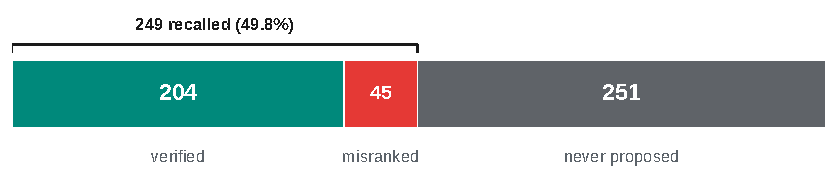
\includegraphics[width=0.92\linewidth]{fig_wall.pdf}
  \caption{Diagnostic wall: \textbf{locked $n{=}194$ instrumented slice}
  (58 verified / 7 mis-ranked / 129 never proposed).
  Expansion-106 has no forward-verify; this is \textbf{not} a pooled $n{=}300$ wall.
  Headline generation recall is 133/300.
  Never-proposed cases bind top-1 despite 89\% conditional precision (58/65).
  Same slice as Figure~\ref{fig:fig1}c.}
  \label{fig:fig-wall}
\end{figure}

\begin{table}[h]
\caption{Locked $n{=}194$ cases from released candidate files.
$^{13}$C chamfers in ppm; Tanimoto Morgan $r{=}2$. IDs are locked-round labels.}
\label{tab:cases}
\centering
\scriptsize
\setlength{\tabcolsep}{3.5pt}
\begin{tabular}{@{}lp{2.15cm}p{8.75cm}@{}}
\toprule
mode & id / formula & what failed \\
\midrule
\textbf{Proposal miss} &
main-R06 / C$_{29}$H$_{30}$FNO$_{2}$ &
True acridinedione never in the 3-candidate pool (Tanimoto-0.90 regioisomer: 4-fluorophenyl/phenyl swapped).
IR 1641, 1510~cm$^{-1}$; $^{13}$C 195.7. Verifier unused. \\
\textbf{Verify-save} &
v3-R25 / C$_{10}$H$_{14}$N$_{2}$O &
True 2-pyridyl picolinamide at self-rank 3; self-rank 1 is 3-pyridyl.
Forward-verify recovers (chamfer 0.42 vs 1.30~ppm). IR 1679~cm$^{-1}$.
Fig.~\ref{fig:fig-mechanism}. \\
\textbf{Verify-fail} &
v3-R26 / C$_{14}$H$_{11}$N$_{3}$O$_{3}$ &
True 3-nitrophenyl dihydroquinazolinone in pool (self-rank 2); 2-nitro ranked first.
Chamfer 1.35 vs 1.36~ppm. IR 1652, 1530, 1352~cm$^{-1}$. \\
\bottomrule
\end{tabular}
\end{table}

\begin{table}[h]
\caption{Expansion round (Claude Opus, InChIKey-14). Five $^{13}$C-overread flags stay in
the $n{=}300$ headline; validate-clean $n{=}295$ in Table~\ref{tab:clean295}.
Incomplete Fable arm (68/106) is never pooled.}
\label{tab:expansion}
\centering
\begin{tabular}{@{}lrr@{}}
\toprule
 & all ($n{=}106$) & clean ($n{=}101$) \\
\midrule
top-1 & 63/106 (59.4\%) & 61/101 (60.4\%) \\
generation recall & 68/106 (64.2\%) & 65/101 (64.4\%) \\
\bottomrule
\end{tabular}
\end{table}

\begin{table}[h]
\caption{Validate-clean sensitivity ($n{=}295$; five $^{13}$C-overread flags excluded).
Same scorer as Table~\ref{tab:headline}; not the headline.}
\label{tab:clean295}
\centering
\scriptsize
\setlength{\tabcolsep}{3pt}
\begin{tabular}{@{}lrrr@{}}
\toprule
metric & overall ($n{=}295$) & simple ($n{=}147$) & complex ($n{=}148$) \\
\midrule
top-1 exact constitution & 116/295 (39.3\%) [34--45] & 59.2\% [51--67] & 19.6\% [14--26] \\
recovered (top-3) & 130/295 (44.1\%) [39--49] & 63.9\% [56--71] & 24.3\% [17--31] \\
scaffold-level (best Tanimoto $\geq 0.45$) & 64\% & 80\% & 48\% \\
mean best Tanimoto & 0.66 & 0.79 & 0.53 \\
\bottomrule
\end{tabular}
\end{table}

By size on $n{=}295$: 67.9\% top-1 at $\leq$15 heavy atoms, 42.8\% at 16--25, 16.7\% above 25
($n{=}53/152/90$).
Full InChIKey (stereo): 93/295 (31.5\%) top-1 [26--37], recall 108/295 (36.6\%) [31--42].
Corpus-reweighted (17.5\% simple / 82.5\% complex): top-1 \textbf{26.5\%} [21--32], recall
\textbf{31.3\%} [25--37].
Self-ranking precision $|$ recall: 116/130 (89.2\%).

\end{document}
 shim for older compile notes.
% main_IRExpBench_only.tex is an optional orphan alternate --- not the ICLR build root.
% Headline n=300 generation (194 locked + all 106 expansion); fig_wall is the n=194 instrumented slice.
% expand-500: 230/230 deposited, unscored --- do not invent top-1 or a pooled wall.
% Compile with pdfLaTeX or XeLaTeX + BibTeX (references.bib + iclr2027_conference.bst).
% \iclrfinalcopy is the only official sty flag that prints \author and drops
% the left-margin submission ruler (see tex/iclr2027_conference.sty).
\documentclass{article}
\usepackage{iclr2027_conference,times}

\usepackage{hyperref}
\usepackage{url}
\usepackage{booktabs}
\usepackage{graphicx}
\usepackage{amsmath,amssymb}
\usepackage{enumitem}
\usepackage{placeins}
\usepackage{xcolor}
\usepackage{listings}
\usepackage{framed}
\lstdefinestyle{benchjson}{
  basicstyle=\ttfamily\scriptsize,
  breaklines=true,
  columns=fullflexible,
  keepspaces=true,
  showstringspaces=false,
  frame=none,
  literate={-}{-}1
}
\setlist{nosep,leftmargin=1.35em}
\setlength{\textfloatsep}{10pt plus 2pt minus 2pt}
\setlength{\floatsep}{8pt plus 2pt minus 2pt}
\setlength{\intextsep}{8pt plus 2pt minus 2pt}

\graphicspath{{figures/}{../figures/}{./}}

% Alternate Overleaf title (not used): Molecular Structure Elucidation with Frontier Models: A Benchmark on Literature-Reported IR, $^1$H, and $^{13}$C NMR Peak Lists
\title{Generation Recall, Not Verification, Binds LLM Structure Elucidation from Literature Spectra}

\author{
Ilkham Yabbarov\textsuperscript{1,$\dagger$},
Rudra Sondhi\textsuperscript{1},
Rodrigo A.\ Vargas-Hern\'andez\textsuperscript{1,2,3,$\dagger$}\\
\textsuperscript{1}Department of Chemistry and Chemical Biology, McMaster University,
Hamilton, Ontario L8S 4L8, Canada.\\
\textsuperscript{2}Brockhouse Institute for Materials Research, McMaster University,
Hamilton, Ontario L8S 4L8, Canada.\\
\textsuperscript{3}School of Computational Science and Engineering, McMaster University,
Hamilton, Ontario L8S 4L8, Canada.\\
$\dagger$\,\textit{E-mail:} yabbaroi@mcmaster.ca, vargashr@mcmaster.ca
}

\newcommand{\fix}{\marginpar{FIX}}
\newcommand{\new}{\marginpar{NEW}}

% Official ICLR 2027 switch: show \author and disable the submission linenumber
% ruler. The same flag also sets the running header to "Published as...".
% Double-blind (submit): keep \iclrfinalcopy commented; \maketitle then prints
% "Anonymous authors / Paper under double-blind review". Camera-ready: uncomment
% \iclrfinalcopy and delete the \lhead override below.
% \iclrfinalcopy  % OFF for double-blind submission; re-enable for camera-ready
\begin{document}

\maketitle
\lhead{Under review as a conference paper at ICLR 2027}

\begin{abstract}
Frontier large language models are often cast as near-solved structure elucidators on
curated spectra. We ask the operational question: given only the molecular formula and
\textbf{literature-reported} IR / $^1$H / $^{13}$C \textbf{peak lists} --- not digitised
traces --- can an off-the-shelf LLM recover constitution, and \textbf{which stage fails}
when it cannot?

The binding claim is \textbf{propose $\gg$ verify}: candidate proposal, not ranking,
is the expensive stage.
We release \textbf{IRSpectra-Bench}, a blind peak-list benchmark of \textbf{300}
compounds (194 locked $+$ all 106 Opus expansion, flags included) drawn from the
companion \textbf{IRexp} band-list resource~\citep{yabbarov2026irexp} --- cited
here, not re-described --- with a fixed RDKit InChIKey-connectivity contract and
decomposable \textbf{generation recall} / \textbf{verification precision} metrics.
A frontier LLM recovers \textbf{39\%} top-1 (118/300; 95\% CI 34--45), or
\textbf{27\%} after corpus reweighting; generation recall is \textbf{44\%} (133/300).
On the forward-verified $n{=}194$ slice the true structure enters the pool for only
\textbf{34\%} of compounds, yet training-free forward-verification selects it
\textbf{89\%} of the time once proposed (58/65).
The expansion slice is easier (59\% vs 28\% top-1) and is disclosed, not hidden.
A larger deposited blind round toward $n{\approx}500$ is \textbf{unscored} and is
not in this headline.
The same recall $\ll$ precision asymmetry replicates across \textbf{four vendor families}.
Formula-only controls collapse; accuracy is flat in source-paper year; generate-wide
sampling lifts recall where verification alone barely moves top-1.
Recovered from published top-$k$ figures, recall carries \textbf{68--83\%} of the accuracy
collapse from curated or simulated spectra to real heterogeneous peak lists.
Frozen predictions, scorers and code are released for mechanical re-evaluation.
\end{abstract}

\section{Introduction}
\label{sec:introduction}

Structure elucidation from spectra sits at the centre of synthetic and analytical chemistry,
and machine learning increasingly treats it as a sequence or agent task.
Encoder--decoder models train on paired corpora~\citep{chacko2024spectro,ottomano2025nmiracle,alberts2024ir};
LLM agents and puzzle benches report high recovery on curated or education
spectra~\citep{kamber2026chemist,guo2024molpuzzle,zhuang2025treesearch,espejo2026agentic}.
Cross-paper numbers swing wildly with harness (e.g.\ GPT-4o from 1.4\% to 57.8\% on MolPuzzle
under different prompting~\citep{guo2024molpuzzle,zhuang2025treesearch}).
What remains under-measured is the harder operational task: \textbf{taking peak lists as
printed in open-access papers and recovering constitution} with an off-the-shelf model,
a fixed molecular-representation scoring contract, and an honest account of
\textbf{which stage of elucidation binds} --- proposal versus verification.

We argue that end-to-end top-1 alone is the wrong reporting primitive.
Any system that returns a ranked candidate list factorises as
\begin{equation}
\text{top-1} \;=\; \underbrace{P(\text{true} \in \text{pool})}_{\text{generation recall}}
\times
\underbrace{P(\text{rank}=1 \mid \text{true} \in \text{pool})}_{\text{verification precision}}.
\end{equation}
These rates have different denominators and must not be differenced.
Prior work already notes that re-ranking cannot recover a missing
candidate~\citep{priessner2026reasoning}; we supply the missing \textbf{measurement
infrastructure at scale}.

\paragraph{Contributions.}
\begin{enumerate}
  \item \textbf{IRSpectra-Bench} --- a blind, complexity-stratified peak-list benchmark ($n{=}300$)
        with a pre-registered InChIKey-connectivity scorer and community reporting contract
        (top-1, generation recall, verification precision $|$ recall).
  \item \textbf{A recall-bound diagnosis} on a frontier LLM: propose $\gg$ verify.
        Generation recall is 44\% on the pooled $n{=}300$ cohort; on the $n{=}194$
        instrumented slice, 34\% proposed and 89\% selected once proposed; that slice's
        top-1 moves only 28\% $\to$ 30\% under training-free forward-verification.
  \item \textbf{Contamination and cross-vendor controls} --- formula-only and recency bounds;
        four-vendor replication of recall $\ll$ precision.
  \item \textbf{A literature decomposition} that recovers the same split from published top-$k$
        figures, showing recall carries most of the collapse on real heterogeneous data.
\end{enumerate}

\paragraph{Dataset pointer (resource, not co-headline).}
Band lists come from the companion \textbf{IRexp} resource (121,233 records; 43,060
structure-linked; 33,201 full IR+$^1$H+$^{13}$C+structure quadruples); an anonymised
review copy is in Appendix~\ref{app:dataset}.
Construction and licensing live in a \textit{Scientific Data} manuscript (in
preparation)~\citep{yabbarov2026irexp}.
This ICLR paper \textbf{cites} that resource and does not re-present a Data Descriptor.

\begin{figure}[t]
  \centering
  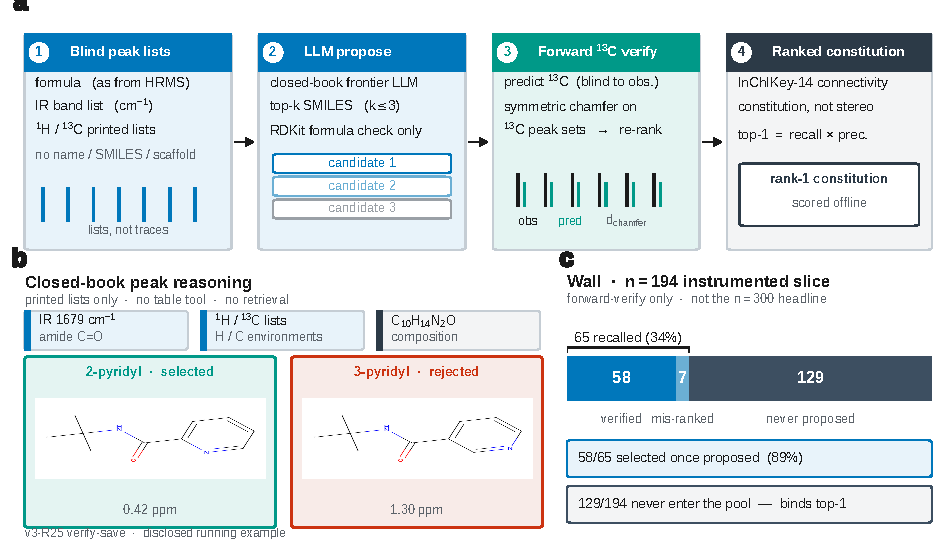
\includegraphics[width=\linewidth]{fig1_overview.pdf}
  \caption{IRSpectra-Bench protocol.
  (a)~Printed IR/$^1$H/$^{13}$C lists $+$ formula $\rightarrow$ closed-book LLM
  proposes top-$k$ SMILES (RDKit formula check) $\rightarrow$ forward $^{13}$C
  (blind) $\rightarrow$ chamfer re-rank $\rightarrow$ InChIKey-14.
  (b)~Evidence is the lists themselves (no peak-table tool, no retrieval).
  Running example v3-R25 (IR 1679~cm$^{-1}$; chamfer 0.42 vs 1.30~ppm).
  (c)~Locked $n{=}194$ instrumented wall: 58 verified / 7 mis-ranked / 129 never
  proposed. \textbf{Not} a pooled $n{=}300$ wall
  (headline generation: Table~\ref{tab:headline}; diagnostic repeat:
  Figure~\ref{fig:fig-wall}).}
  \label{fig:fig1}
\end{figure}

\section{Related work}
\label{sec:related-work}

\paragraph{Trained spectra $\to$ structure models.}
Sequence and graph decoders on paired
corpora~\citep{chacko2024spectro,hu2024multitask,yang2026nmrtrans,ottomano2025nmiracle,alberts2024ir,alberts2025benchmarks}
are accurate in-distribution but typically scored end-to-end.
We do not claim to beat them on IRSpectra-Bench; Spectro, NMIRacle, Alberts IR transformers
and CASE are \textbf{not yet scored} on our bench (Section~\ref{sec:limitations}) --- a gap we
state honestly and leave to the released scorer.

\paragraph{Agentic elucidation: three regimes.}
The contrast is the \textbf{setting and the stage split}, not a method scoreboard.
(i)~\emph{Tool-using lab agents} --- ChemCrow~\citep{mbran2024chemcrow},
Coscientist~\citep{boiko2023coscientist} --- show that LLMs can call instruments and
planners; they do not measure which elucidation stage binds.
(ii)~\emph{Spectrum-native agents} improve \emph{how} a model reads a spectrum or
re-ranks a \textbf{fixed} pool: tree-search~\citep{zhuang2025treesearch},
SpecMol~\citep{shen2025specmol}, Priessner \textit{et al.}~\citep{priessner2026reasoning},
NMR-Solver~\citep{jin2025nmrsolver}, NMRAgent~\citep{fang2026nmragent}.
Priessner already notes that re-ranking cannot recover a missing candidate; we measure
that failure at literature-peak-list scale.
SpectraLLM~\citep{su2025spectrallm} is a \textbf{fine-tuned} multi-spectral elucidator
on \textbf{simulated} corpora (QM9S DFT; Alberts USPTO multimodal) --- a different object
and a different training regime; we do not score it here.
IR-Agent~\citep{noh2025iragent} (ICLR 2026) is the closest concurrent multi-agent IR
elucidator: on \textbf{NIST experimental IR} a translator proposes a SMILES pool, TI+Ret
enrich local (peak-table) and global (retrieved-spectrum) features, and an SE expert
re-ranks (Top-$k$ SMILES; atom type / scaffold / carbon count may be prompt-injected).
(iii)~\emph{Agentic-search benches} --- MolQuest~\citep{han2026molquest},
NMRGym~\citep{fang2026nmrgym}, Espejo Morales \textit{et al.}~\citep{espejo2026agentic}
(education $\to$ industrial instrument files: 80.9\% $\to$ 20.6\%) --- ask which
architecture or abductive loop wins.
IRSpectra-Bench is the harder operational object: \textbf{literature peak lists}
(IR+$^1$H/$^{13}$C+formula as from HRMS), \textbf{off-the-shelf} closed-book models, no
name, SMILES, or scaffold hint.
We measure \textbf{which stage binds} after spectra are read --- generation recall versus
verification precision $|$ recall --- on pooled $n{=}300$, with instrumented
forward-verify on $n{=}194$.
IR-Agent's SE expert over a \textbf{fixed candidate pool} is exactly the regime our
ladder diagnoses as recall-limited (proposal binds; conditional forward-verify
$\approx$89\%, 58/65).
TI+Ret can enrich \emph{features} but does \textbf{not} remove a proposal wall if the true
structure never enters the pool.
Architecture search that does not change $P(\text{true}\in\text{pool})$ cannot move
top-1 on a recall-bound bench.
We do not claim to beat SpectraLLM or IR-Agent on their native sets; neither is scored
here.
\begin{center}
\scriptsize
\setlength{\tabcolsep}{4pt}
\begin{tabular}{@{}llll@{}}
\toprule
 & input & metric & binds \\
\midrule
IR-Agent & NIST experimental IR & Top-$k$ SMILES & re-rank given pool \\
this paper & lit.\ IR+$^1$H/$^{13}$C+formula lists & recall vs prec.$|$recall & proposal \\
\bottomrule
\end{tabular}
\end{center}

\paragraph{Heterogeneous data, CASE, and positioning.}
Most prior suites use simulated or single-instrument spectra; we use literature-reported
peak lists across thousands of laboratories and report formula-only and recency controls
(Section~\ref{sec:contamination}).
Matching predicted to observed shifts --- DP4~\citep{smith2010dp4},
CASE~\citep{elyashberg2012case}, NMR-Solver, NMRAgent --- is easier than inverse
generation; CASE enumerators have exhaustive recall by construction, while the LLM
literature almost never reports whether the true structure was proposed at all.
SpecX~\citep{xiang2026specx} bounds a related multi-modal spectroscopy task on
simulated traces.
IRSpectra-Bench is an openly redistributable literature-peak-list suite with a
\textbf{stage decomposition}, measured on Claude and replicated across three other
model families.

\FloatBarrier
\section{IRSpectra-Bench}
\label{sec:benchmark}

\subsection{Task and inputs}

Each of 300 problems supplies the \textbf{molecular formula} (as from HRMS), the \textbf{IR
band list} (cm$^{-1}$), and \textbf{$^1$H / $^{13}$C shift lists} --- exactly the textual form
reported in open-access papers.
No name, SMILES or scaffold hint.
Inputs are author-transcribed \textbf{band and shift lists}, not absorbance traces or FIDs:
a different object from digitised-spectrum benchmarks~\citep{espejo2026agentic}, and one that
matches how language models consume literature.

The cohort is the pre-registered pool of a locked 194 (spectrally validated main round 134 $+$
60 controls) and a 106-compound expansion draw ($n{=}300{=}194{+}106$).
Five expansion records fail the same $^{13}$C-overread audit used on the main round and are
included in the 300 (validate-clean $n{=}295$ in Appendix~\ref{app:extended}).
Problems are drawn from the structure-complete split of IRexp (\texttt{irexp\_resolved}; see
companion Data Descriptor)~\citep{yabbarov2026irexp}.
On the locked 194, author peak assignments name a ring system in 10/194; those are solved
1/10 vs 54/184 for the rest, so named-ring annotation does not drive that slice.
Figure~\ref{fig:fig-chemspace} summarises the chemistry space of the pooled headline.
Figure~\ref{lst:payload} is the solver-facing contract: formula plus printed peak lists,
gold constitution held out.

\begin{figure}[ht]
  \centering
  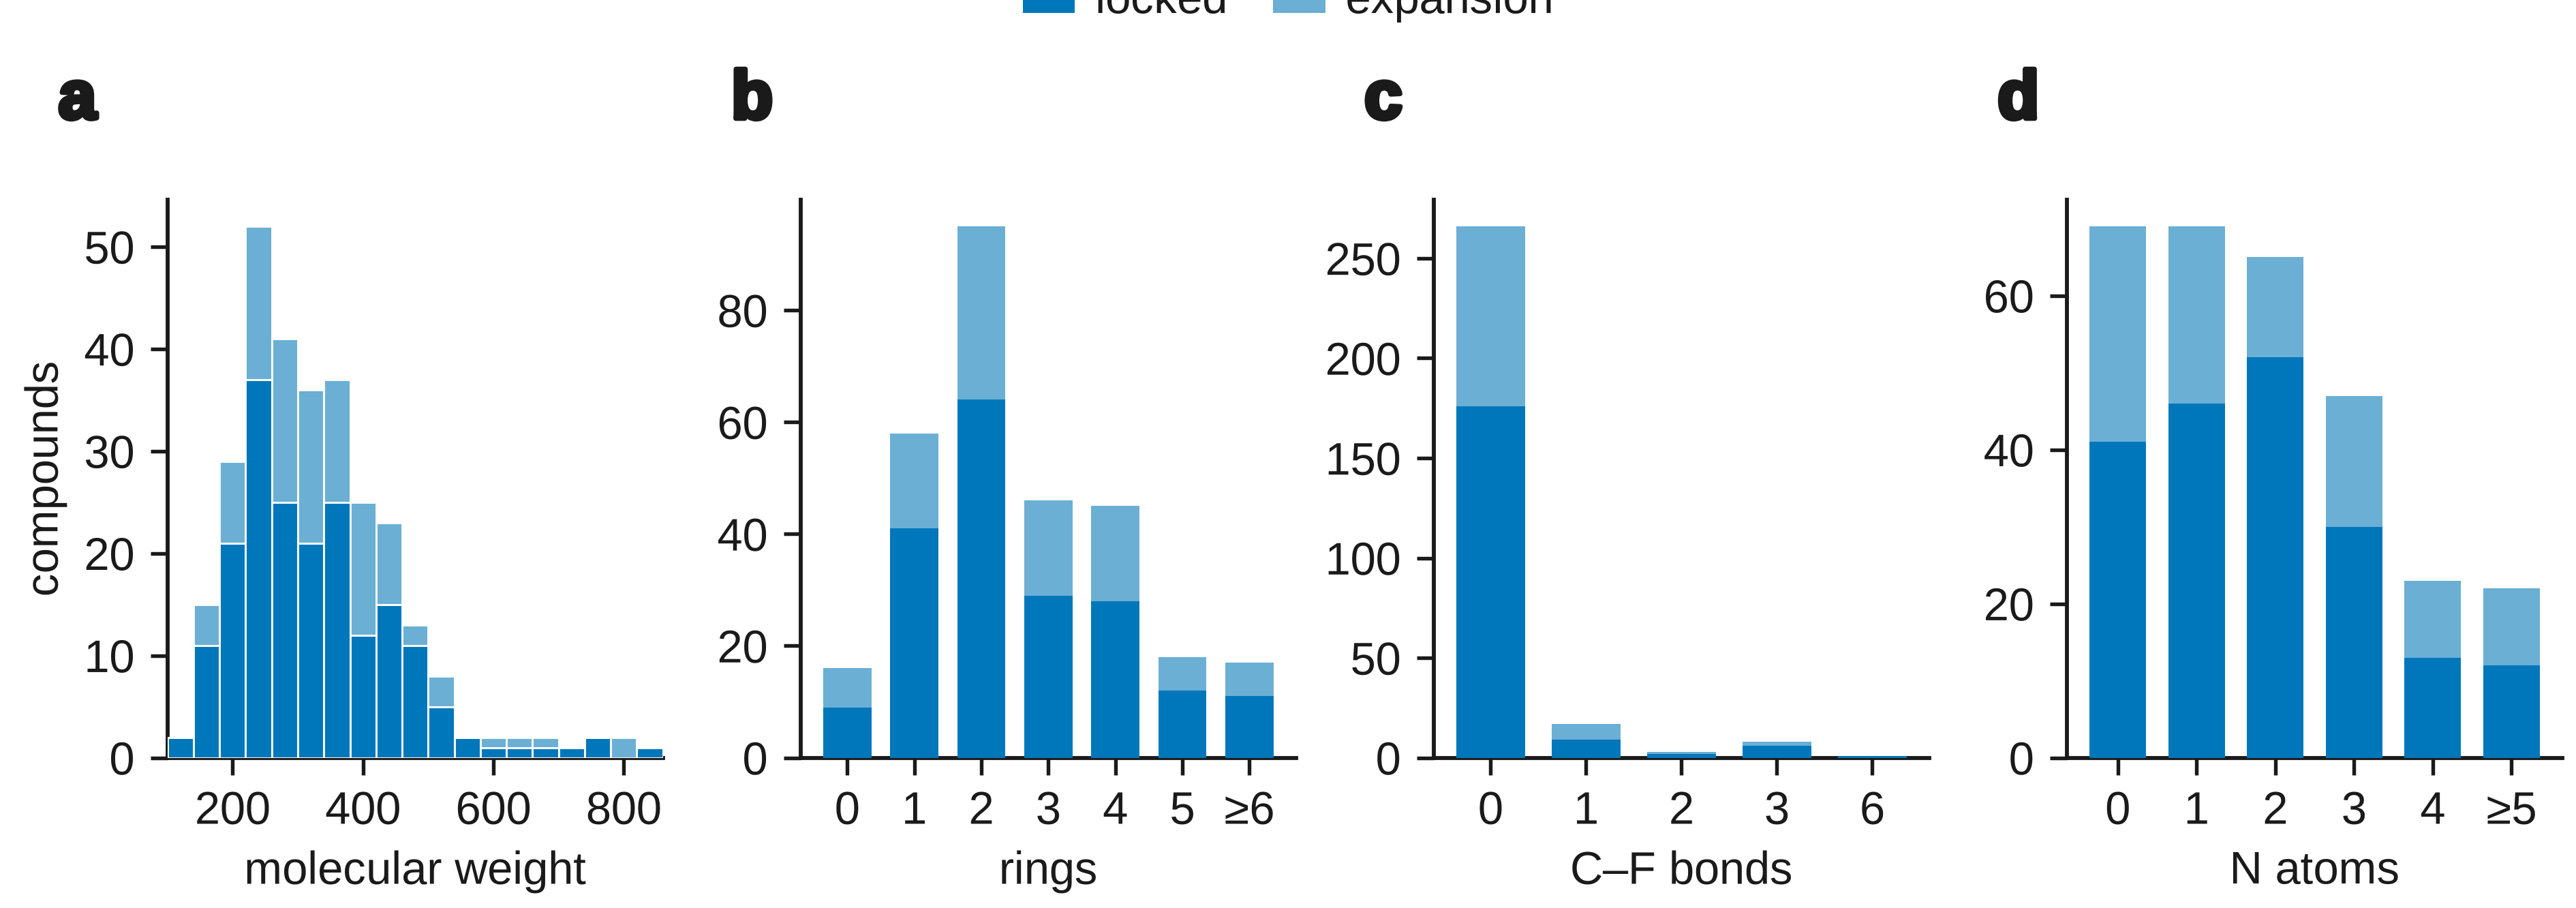
\includegraphics[width=0.92\linewidth]{fig_chemspace.png}
  \caption{Pooled headline chemistry ($n{=}300$; panels on validate-clean $n{=}295$).
  (a)~MW (median 306). (b)~RDKit rings (median 2). (c)~C--F bonds. (d)~N atoms.
  Stacked: locked (dark) vs expansion (light). Mid-size literature space, not a NIST toy set.}
  \label{fig:fig-chemspace}
\end{figure}

\subsection{Difficulty, balance, and scoring contract}

\textbf{Difficulty} is declared \emph{a priori} by RDKit ring analysis: \emph{simple} iff
$\leq$2 rings, no fused/spiro/bridgehead system, $\leq$22 heavy atoms; else \emph{complex}
(151/149 on $n{=}300$).
The released benchmark is \textbf{50/50 by design}; the eligible corpus is 17.5\% simple /
82.5\% complex.
Reweighted to corpus composition on the validate-clean subset, top-1 falls 39.3\% $\to$
\textbf{26.5\%} [21--32] and recall 44.1\% $\to$ \textbf{31.3\%} [25--37]
(Appendix~\ref{app:extended}).
We report both: the reweighted figure is the better estimate for an arbitrary paper, and the
50/50 figure is the comparable leaderboard number (Table~\ref{tab:headline}).

\textbf{Scoring.} A prediction is correct if RDKit InChIKey \textbf{connectivity} (first 14
characters) matches --- we score \emph{constitution}.
Full stereo-sensitive InChIKey is reported on the validate-clean subset
(Appendix~\ref{app:extended}).
External submissions: up to three ranked SMILES per \texttt{qid}, no structure hints
(\texttt{docs/LEADERBOARD.md}; \texttt{scripts/score\_submission.py}).
Primary metrics (report all three): \textbf{top-1} (best-ranked candidate matches at
connectivity); \textbf{generation recall} (reference in the pool \emph{before} re-ranking);
\textbf{verification precision $|$ recall} (correct top-1 among recall-positive compounds).
Confidence intervals are bootstrap 95\%; paired model differences use McNemar with Holm correction.

\section{Experimental setup}
\label{sec:setup}

\paragraph{Blind payload and solver.}
The solver sees four JSON fields per \texttt{qid}: \texttt{formula} (as from HRMS),
\texttt{ir\_bands\_cm-1}, \texttt{h\_nmr}, \texttt{c\_nmr} --- peak lists as printed
(Figure~\ref{lst:payload}).
No name, SMILES, scaffold, atom-type hint, or retrieved spectrum; ground truth is scored
offline.
Frontier LLM agent (Claude Opus via consumer subscription), closed-book, one sub-agent per
batch, RDKit formula check only.
No fine-tuning, no paid API, \textbf{no thinking tier} for the core protocol.
Inference is \textbf{not} exactly reproducible (no pinned snapshot, temperature or seed ---
Section~\ref{sec:limitations}).
\textbf{Scoring is reproducible}: frozen predictions, ground truth and scorers regenerate every
training-free number.

\begin{figure}[ht]
\centering
\begin{minipage}{0.98\linewidth}
\begin{framed}
\noindent
\begin{minipage}[c]{0.56\linewidth}
\begin{lstlisting}[style=benchjson]
{
  "qid": "v3-R25",
  "formula": "C10H14N2O",
  "ir_bands_cm-1": [1679, "..."],
  "h_nmr": "[printed 1H list]",
  "c_nmr": "[printed 13C list]"
}
\end{lstlisting}
\end{minipage}\hfill
\begin{minipage}[c]{0.40\linewidth}
\centering
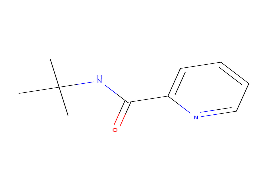
\includegraphics[width=\linewidth]{fig_listing_mol.pdf}\\[0.2em]
{\scriptsize\itshape gold held out}\\[-0.1em]
{\scriptsize 2-pyridyl picolinamide}
\end{minipage}
\end{framed}
\end{minipage}
\caption{\textbf{Listing 1.} Solver-facing payload (abridged), IRexp
JSON$+$molecule layout. Gold constitution (right) is held out.
Only disclosed fragments are shown (v3-R25 / C$_{10}$H$_{14}$N$_{2}$O / IR 1679);
full lists ship with the bench. Source: IRexp~\citep{yabbarov2026irexp};
this PDF is not a Data Descriptor.}
\label{lst:payload}
\end{figure}

\paragraph{Scoring contract and candidate budget.}
A deposit is JSONL of \texttt{\{qid, candidates: [SMILES,\ldots]\}} under a stated budget.
The scorer reports the three Section~\ref{sec:benchmark} metrics at InChIKey-connectivity,
with bootstrap 95\% CIs.
Self-ranking vs forward-verified re-ranking must be labelled; they are not interchangeable.
Headline protocol: $\leq$3 ranked SMILES per \texttt{qid}.
On the 60-compound arm Claude returned mean 2.20 candidates vs 3.00 for the other vendors
(recall rankings approximate).
\textbf{Generate-wide} (that arm only): ten independent solvers $\times$ up to six SMILES,
pooled then re-ranked --- not the $n{=}300$ reporting budget.

\paragraph{Forward-verification, expansion, and probes.}
Generate $\to$ forward-predict $^{13}$C (blind to the observed list) $\to$ re-rank by
symmetric chamfer on $^{13}$C peak sets (Section~\ref{sec:forward-verify}); instrumented on
the locked $n{=}194$ only.
Expansion is a pre-registered 106-compound draw from the same \texttt{irexp\_resolved}
sampler after the $n{=}194$ lock, with the same $^{13}$C-overread audit
(Section~\ref{sec:expansion}): five flags stay in the $n{=}300$ headline; validate-clean
$n{=}295$ is appendix; expansion-106 forward-verify was not run.
A later 230-compound draw toward $n{\approx}500$ is deposited and unscored
(Section~\ref{sec:expansion}).
Controls: formula-only / recency (Section~\ref{sec:contamination}); four-vendor replication
on a 60-compound arm (Section~\ref{sec:cross-vendor}); generate-wide sampling; HOSE lookup
and GNN $^{13}$C verifiers; small IRexp-fine-tuned generator probe (excluded from headline
claims).

\section{Results}
\label{sec:results}

\subsection{Headline performance}
\label{sec:headline}

\begin{table}[ht]
\caption{Headline elucidation ($n{=}300{=}194$ locked $+$ $106$ expansion).
Bootstrap 95\% CIs; validate-clean $n{=}295$ in Appendix~\ref{app:extended}.}
\label{tab:headline}
\centering
\small
\begin{tabular}{@{}lr@{}}
\toprule
metric & $n{=}300$ \\
\midrule
top-1 exact constitution & \textbf{39.3\%} (118/300) [34--45] \\
\quad simple ($n{=}151$) & 58.3\% (88/151) \\
\quad complex ($n{=}149$) & 20.1\% (30/149) \\
generation recall (top-3) & \textbf{44.3\%} (133/300) [39--50] \\
\bottomrule
\end{tabular}
\end{table}

On the validate-clean subset, scaffold-level recovery is 64\% (simple 80\%, complex 48\%) and
mean best Tanimoto is 0.66; accuracy falls with size (67.9\% top-1 at $\leq$15 heavy atoms,
42.8\% at 16--25, 16.7\% above 25; $n{=}53/152/90$; Appendix~\ref{app:extended}).
On the locked 194, of 137 analysable top-1 misses, \textbf{76.6\%} are constitutional isomers of the true
structure; only \textbf{22.6\%} share the true Murcko scaffold --- wrong connectivity at the
right composition, not mostly fine regiochemistry (not re-run on the expansion).
A 24-compound four-model Claude comparison is capability-sensitive (Haiku $\subset$ Sonnet
$\subset$ Opus $\subset$ Fable) but underpowered for adjacent ranks, with a disclosed protocol
asymmetry (Section~\ref{sec:limitations}); a battery-electrolyte subset ($n{=}46$) matches the
locked-slice regime (26\% top-1; recall-bound).

\begin{table}[ht]
\caption{Generation by slice. Headline is pooled $n{=}300$, not locked 194 alone.}
\label{tab:slices}
\centering
\small
\begin{tabular}{@{}lrrr@{}}
\toprule
 & locked ($n{=}194$) & expansion ($n{=}106$) & pooled ($n{=}300$) \\
\midrule
top-1 & 55/194 (28.4\%) & 63/106 (59.4\%) & \textbf{118/300 (39.3\%)} \\
generation recall & 65/194 (33.5\%) & 68/106 (64.2\%) & \textbf{133/300 (44.3\%)} \\
\bottomrule
\end{tabular}
\end{table}

The expansion slice is easier for this solver than the locked 194 (59.4\% vs 28.4\% top-1);
pooling does not hide that gap.
Self-ranking precision $|$ recall on the pooled generation cohort is 118/133 (88.7\%) ---
that is \emph{not} forward-verification precision (Section~\ref{sec:forward-verify}).

\subsection{Is the model reading the spectra?}
\label{sec:contamination}

\begin{table}[ht]
\caption{Formula-only control (paired, $n{=}60$).}
\label{tab:formula-only}
\centering
\small
\begin{tabular}{@{}lrr@{}}
\toprule
condition & top-1 & recovered (top-3) \\
\midrule
formula only & \textbf{3/60 (5\%)} & 3/60 (5\%) \\
formula + IR + $^1$H + $^{13}$C & 14/60 (23\%) & 19/60 (32\%) \\
\bottomrule
\end{tabular}
\end{table}

Outcomes are perfectly nested (McNemar $p{=}0.001$).
Accuracy is flat in source-paper year across the locked 194 ($r{=}{-}0.007$), bounding pretraining
recall of specific papers.
We claim a \textbf{strong bound, not exclusion} of contamination
(Section~\ref{sec:limitations}).

\begin{figure}[ht]
  \centering
  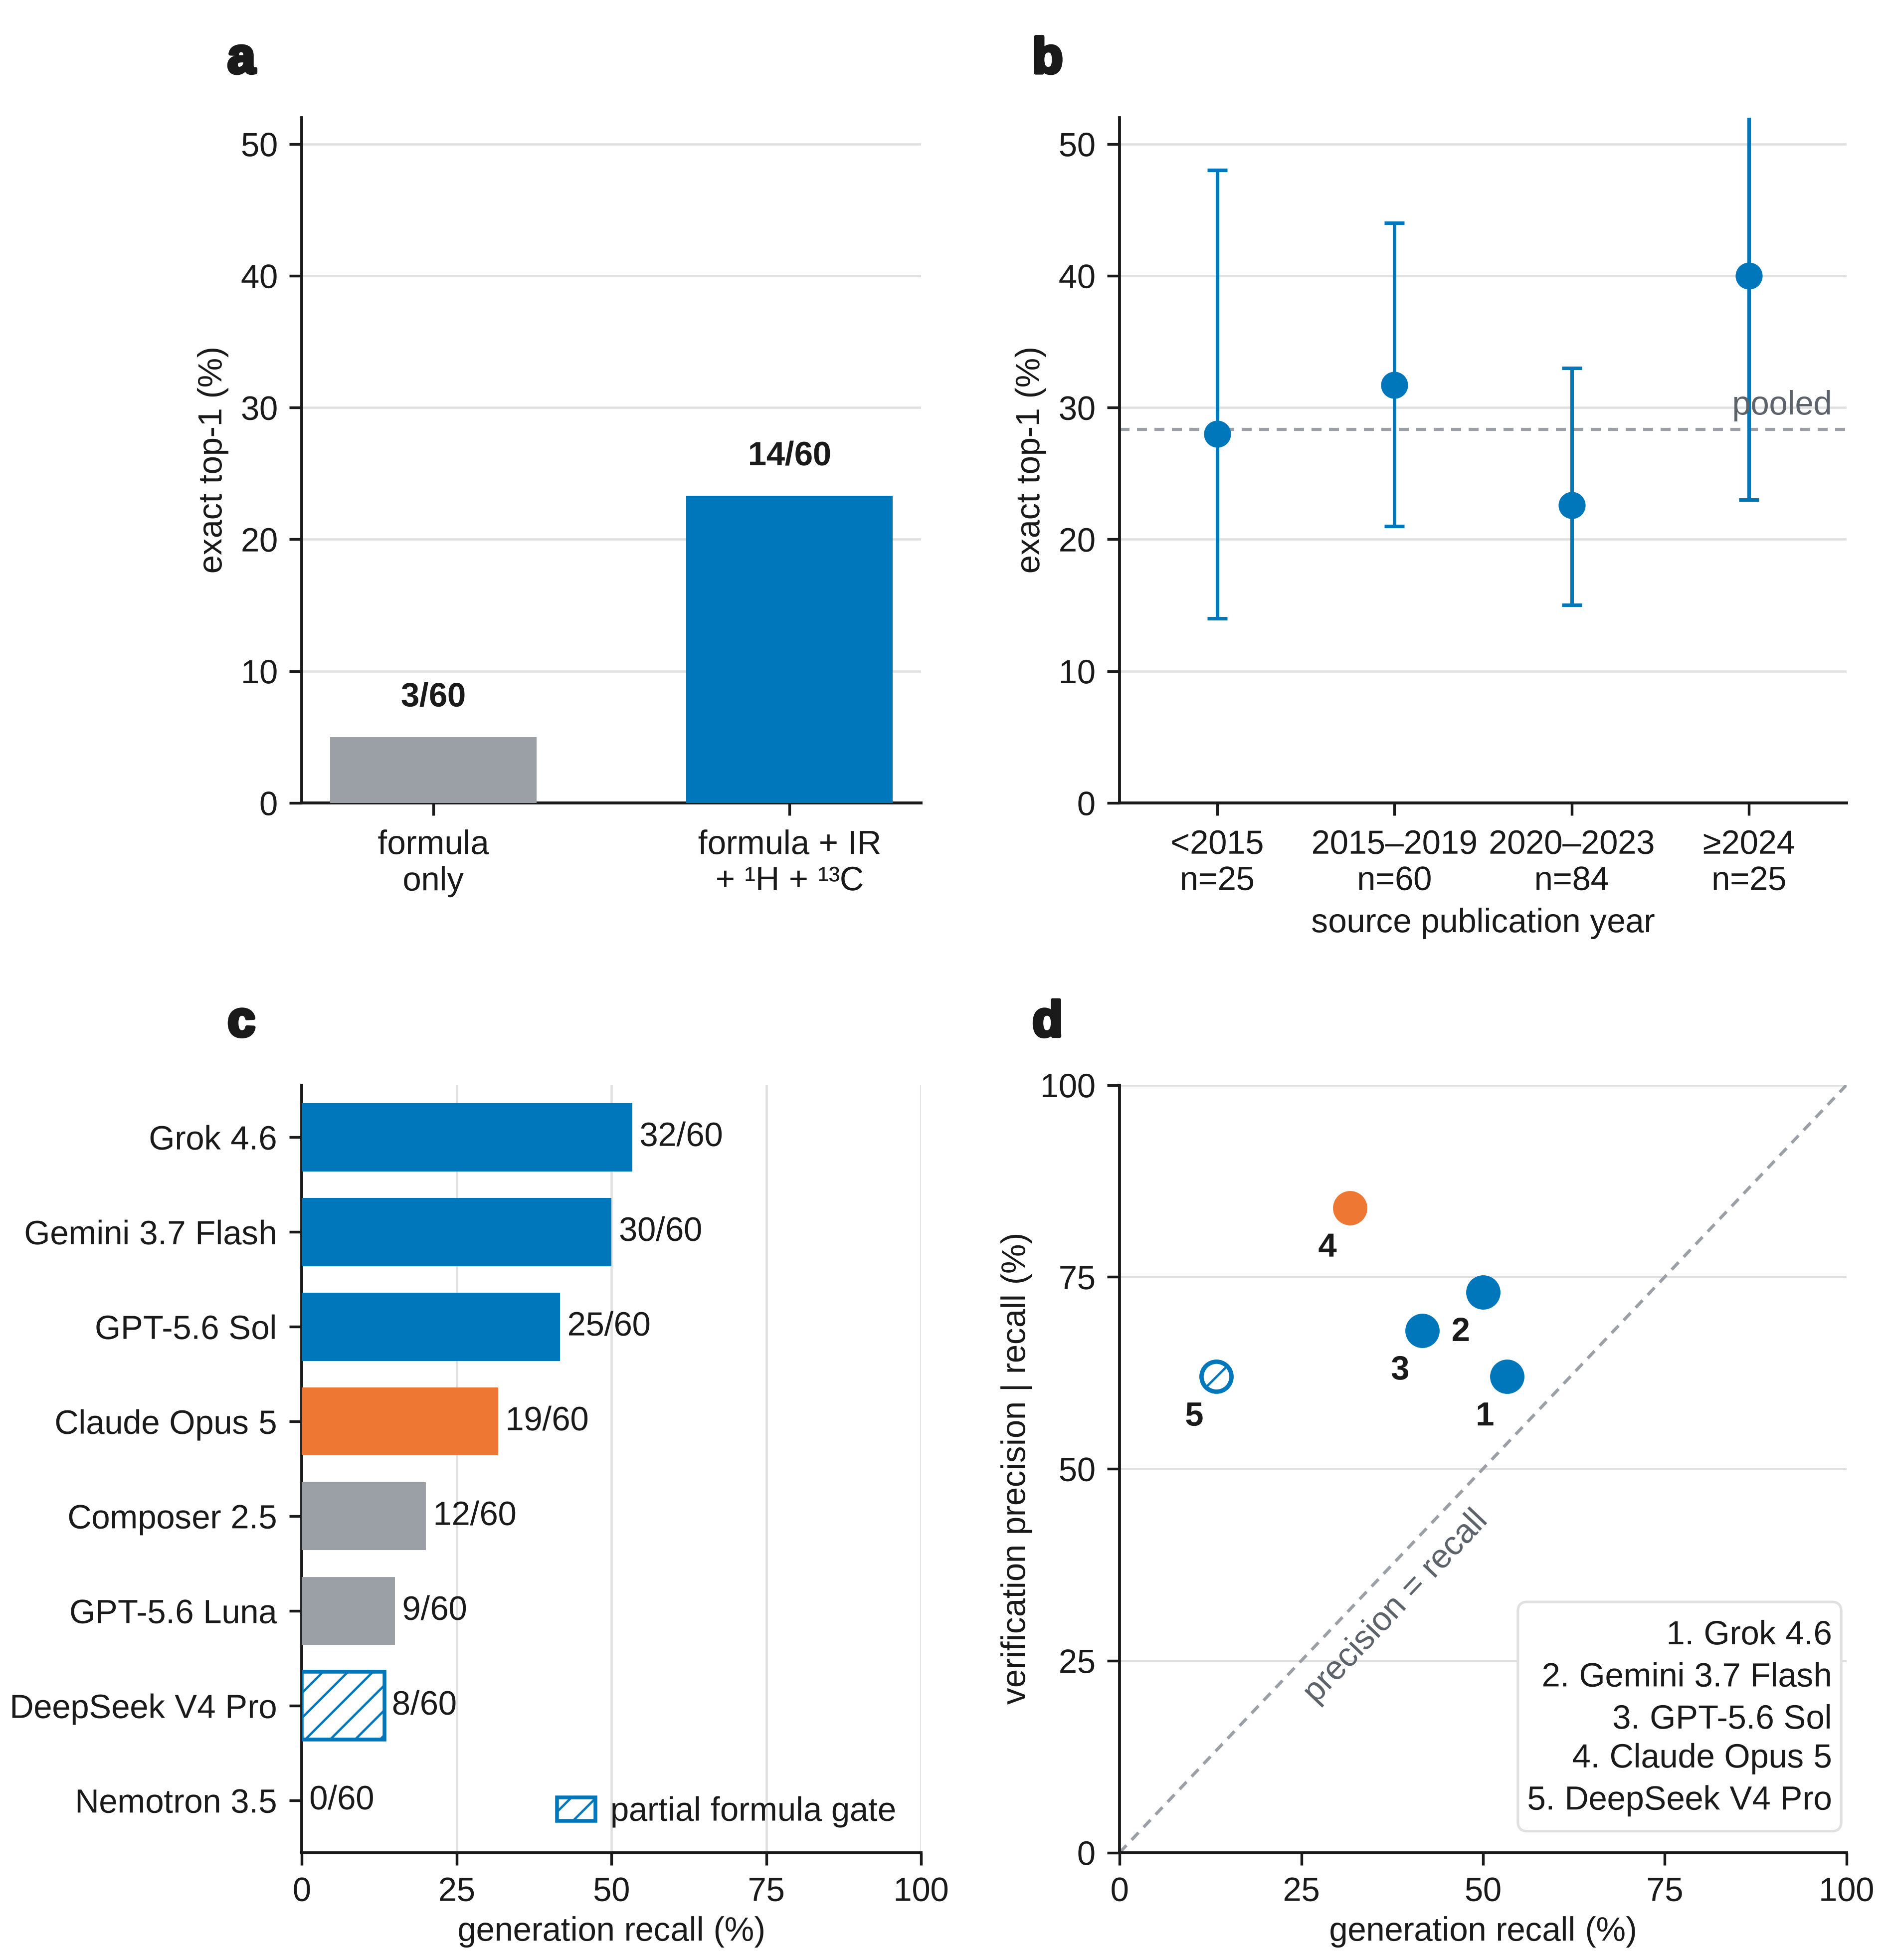
\includegraphics[width=0.62\linewidth]{fig_robustness.png}
  \caption{Robustness on instrumented arms (formula-only / cross-vendor $n{=}60$;
  recency $n{=}194$): formula-only collapse, flat recency, four-vendor recall $\ll$ precision.}
  \label{fig:fig-robustness}
\end{figure}

\subsection{Cross-vendor replication}
\label{sec:cross-vendor}

Grok 4.6, Gemini 3.7 Flash and GPT-5.6 Sol solved the same 60-compound arm under the
identical protocol.
\textbf{Verification precision exceeds generation recall in every arm}; bootstrapping
separates the paired gap for Claude (+52.5 points), GPT-5.6 Sol (+26.3) and Gemini (+23.3);
Grok's gap (+9.2) is directional.

\begin{table}[ht]
\caption{Cross-vendor decomposition ($n{=}60$). Recall and precision use different denominators.}
\label{tab:cross-vendor}
\centering
\small
\begin{tabular}{@{}lrrr@{}}
\toprule
model & generation recall & verification precision $|$ recall & multi-candidate only \\
\midrule
Claude Opus & 19/60 = 32\% & 16/19 = 84\% & 10/13 = 77\% \\
Grok 4.6 & 32/60 = 53\% & 20/32 = 62\% & 20/32 = 62\% \\
Gemini 3.7 Flash & 30/60 = 50\% & 22/30 = 73\% & 22/30 = 73\% \\
GPT-5.6 Sol & 25/60 = 42\% & 17/25 = 68\% & 16/24 = 67\% \\
\bottomrule
\end{tabular}
\end{table}

Candidate budgets differ (Claude mean 2.20 vs others 3.00), so recall rankings are
approximate.
A clean-clone control for Grok bounds key leakage (McNemar $p{=}0.39$).

\subsection{Forward-verification decomposition}
\label{sec:forward-verify}

\begin{figure}[ht]
  \centering
  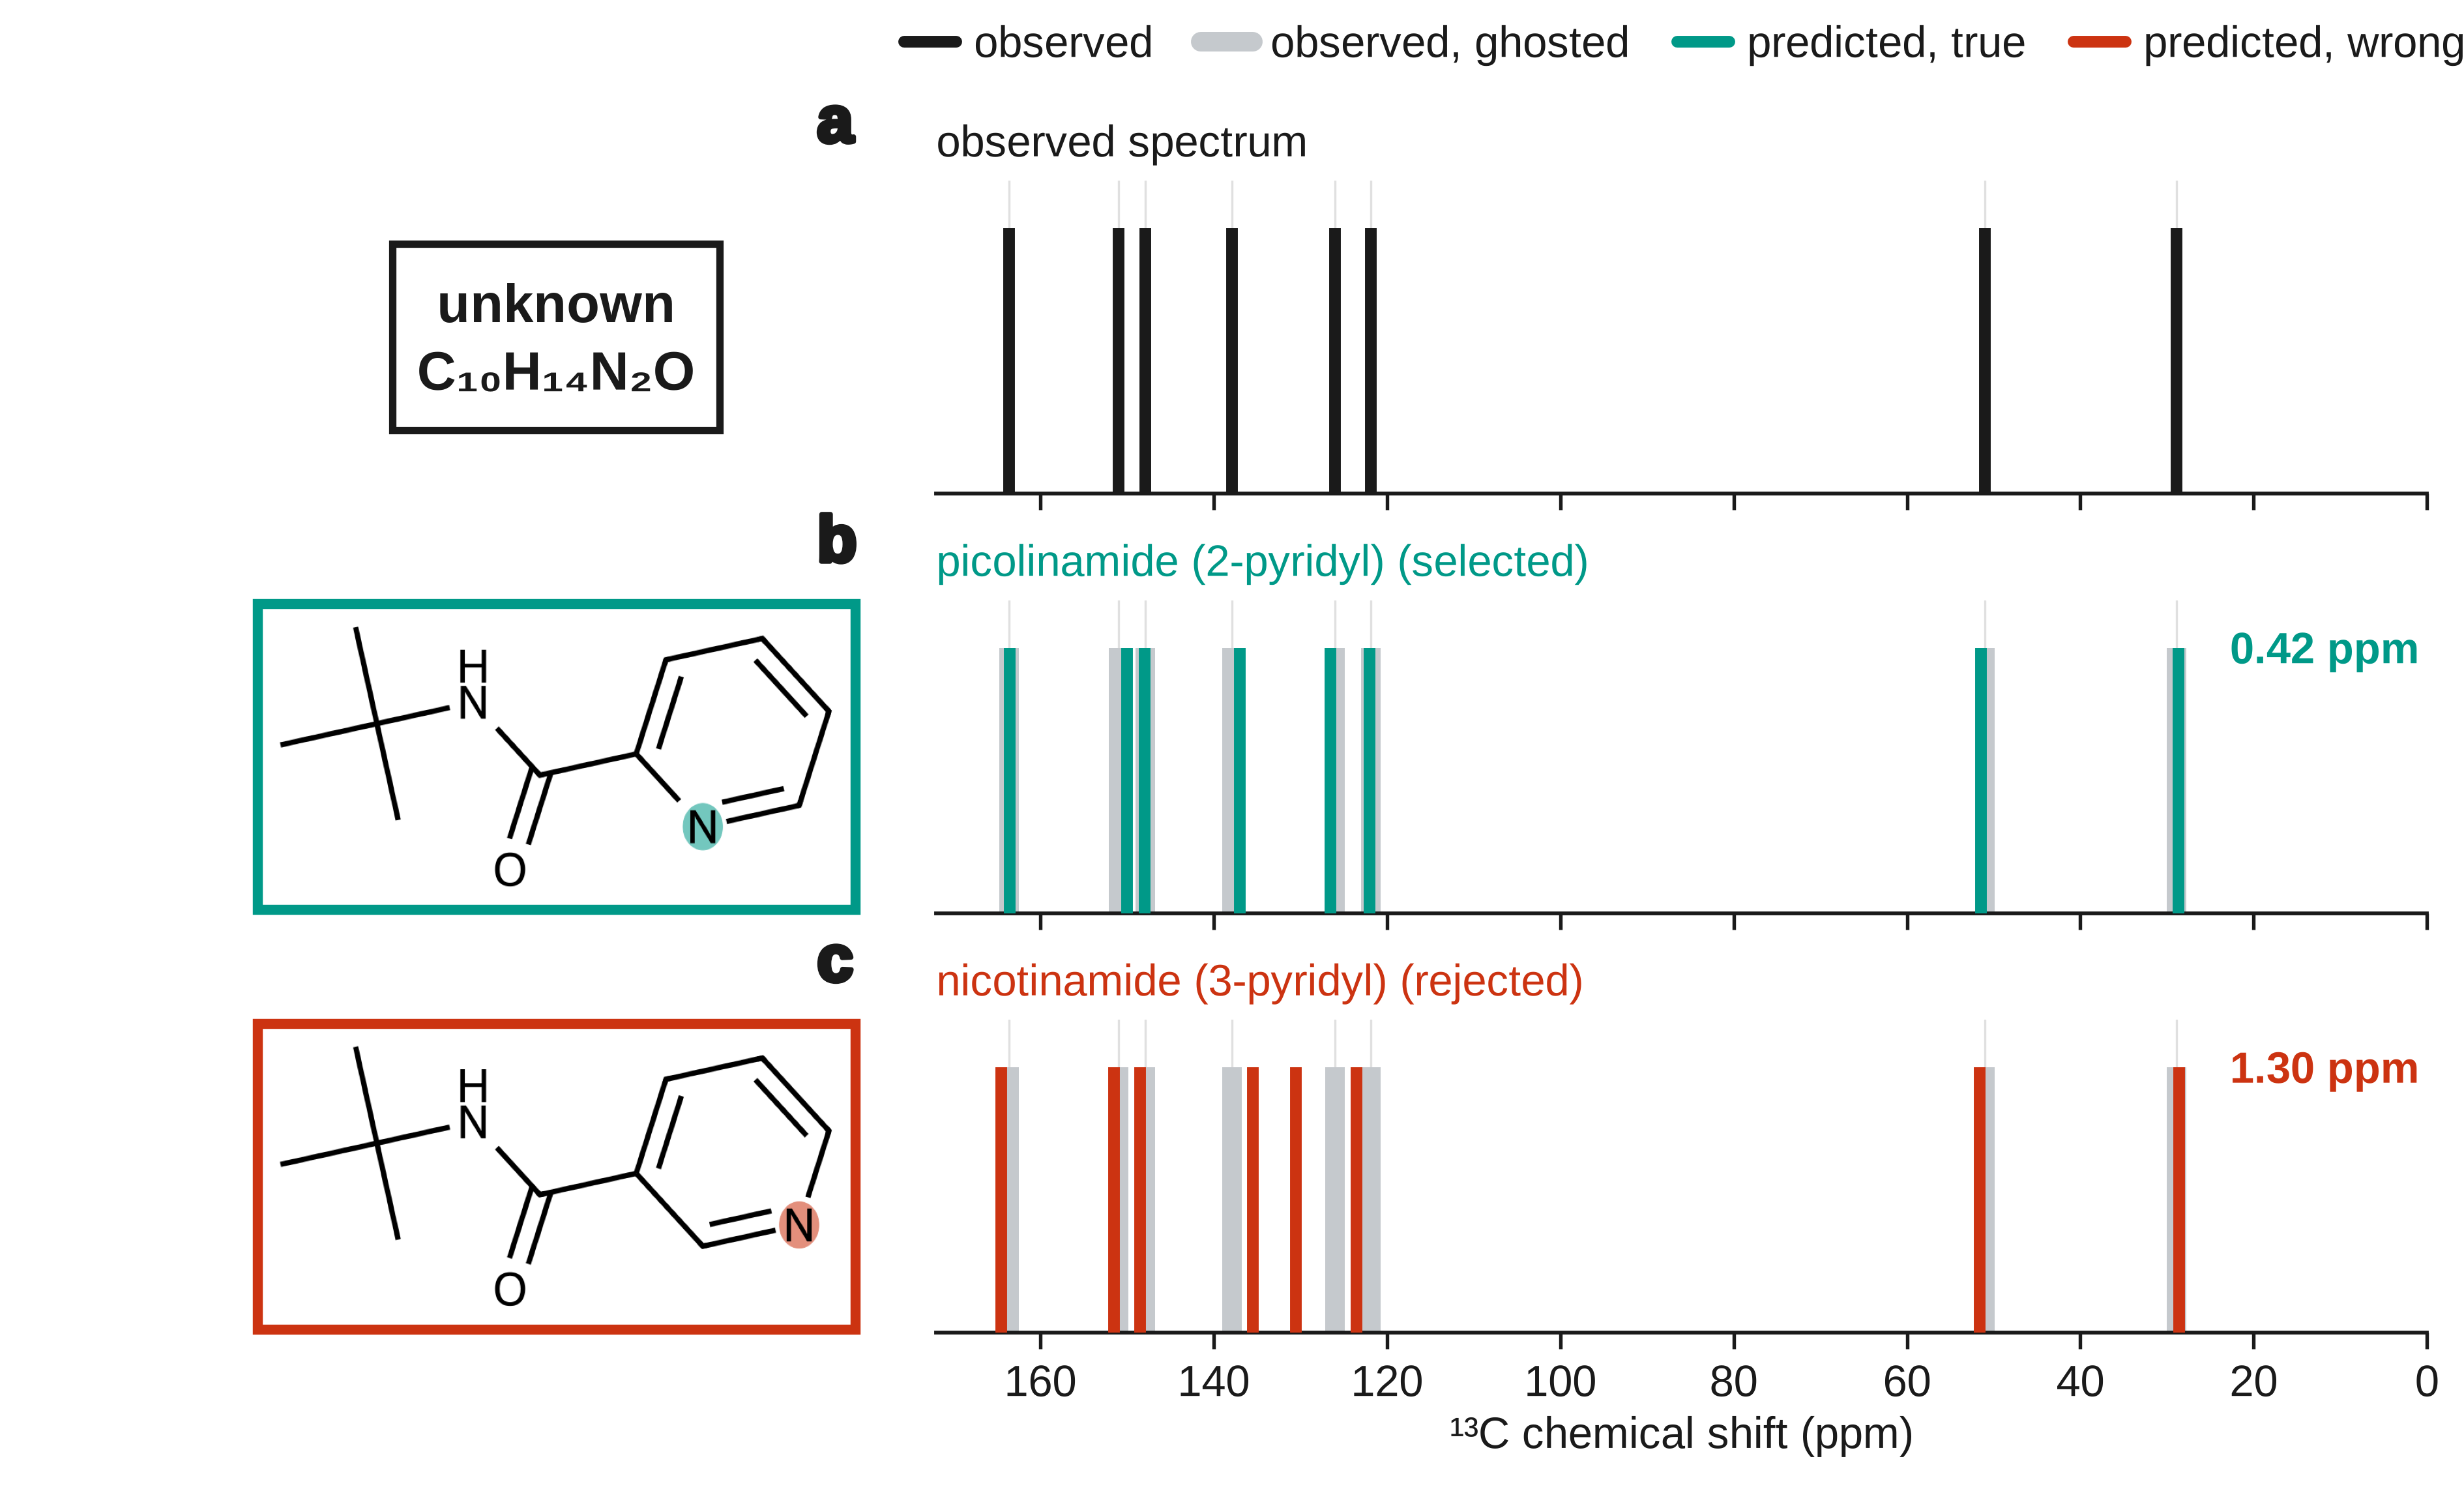
\includegraphics[width=0.72\linewidth]{fig_mechanism.png}
  \caption{Locked v3-R25: self-rank prefers 3-pyridyl; forward $^{13}$C recovers 2-pyridyl
  (chamfer 0.42 vs 1.30~ppm) --- a verify-save, not a recall win (Table~\ref{tab:cases}).}
  \label{fig:fig-mechanism}
\end{figure}

\begin{table}[ht]
\caption{Forward-verify on the instrumented slice ($n{=}194$).
Pooled $n{=}300$ in Table~\ref{tab:headline} is generation only.}
\label{tab:fverify}
\centering
\small
\begin{tabular}{@{}lrr@{}}
\toprule
 & 60-compound arm & locked slice ($n{=}194$) \\
\midrule
generation recall & 19/60 (32\%) & 65/194 (34\%) \\
top-1, solver self-ranking & 14/60 (23\%) & 55/194 (28\%) \\
top-1, forward-verified re-ranking & 16/60 (27\%) & 58/194 (30\%) \\
precision $|$ recall --- forward-verification & 16/19 (84\%) & 58/65 (\textbf{89\%}) \\
multi-candidate only --- forward-verification & 10/13 (77\%) & 30/37 (81\%) \\
\bottomrule
\end{tabular}
\end{table}

When the true structure is among the candidates, forward-verification selects it in 58/65
cases (89\%).
Where a choice existed ($n{=}37$), forward-verification is correct on 30/37 (81\%) against a
54.0\% derangement floor (+27.1 points).
The margin over self-ranking is \textbf{small and unresolved} (seven gained, four lost;
McNemar $p{=}0.55$) --- we do \textbf{not} claim an accuracy advance.
Precision is high while recall binds: no re-ranking repairs the 129/194 compounds on this
slice where the true structure was never proposed (Figure~\ref{fig:fig1}c;
diagnostic repeat in Figure~\ref{fig:fig-wall}).

\paragraph{Worked cases.}
Three locked-slice deposits instantiate the wall (Appendix Table~\ref{tab:cases}; expansion
qids reuse R22/R25 --- IDs below are locked-round labels).
\textbf{main-R06} (C$_{29}$H$_{30}$FNO$_{2}$): true acridinedione never enters the 3-candidate
pool (Tanimoto-0.90 regioisomer); verifier unused.
\textbf{v3-R25} (C$_{10}$H$_{14}$N$_{2}$O): verify-save --- self-rank prefers 3-pyridyl,
forward $^{13}$C recovers 2-pyridyl (chamfer 0.42 vs 1.30~ppm; Figure~\ref{fig:fig-mechanism}).
\textbf{v3-R26} (C$_{14}$H$_{11}$N$_{3}$O$_{3}$): verify-fail --- true 3-nitrophenyl isomer in
the pool but 2-nitro ranked first (chamfer 1.35 vs 1.36~ppm).

\paragraph{Generate-wide.}
Ten solver agents, up to six candidates each, pooled and re-ranked on the 60-compound arm:
recall 32\% $\to$ \textbf{42\%}, top-1 23\% $\to$ \textbf{30\%} (McNemar $p{=}0.34$);
verification precision falls 84\% $\to$ 72\%.
The training-free ceiling remains recall-limited.

\begin{figure}[ht]
  \centering
  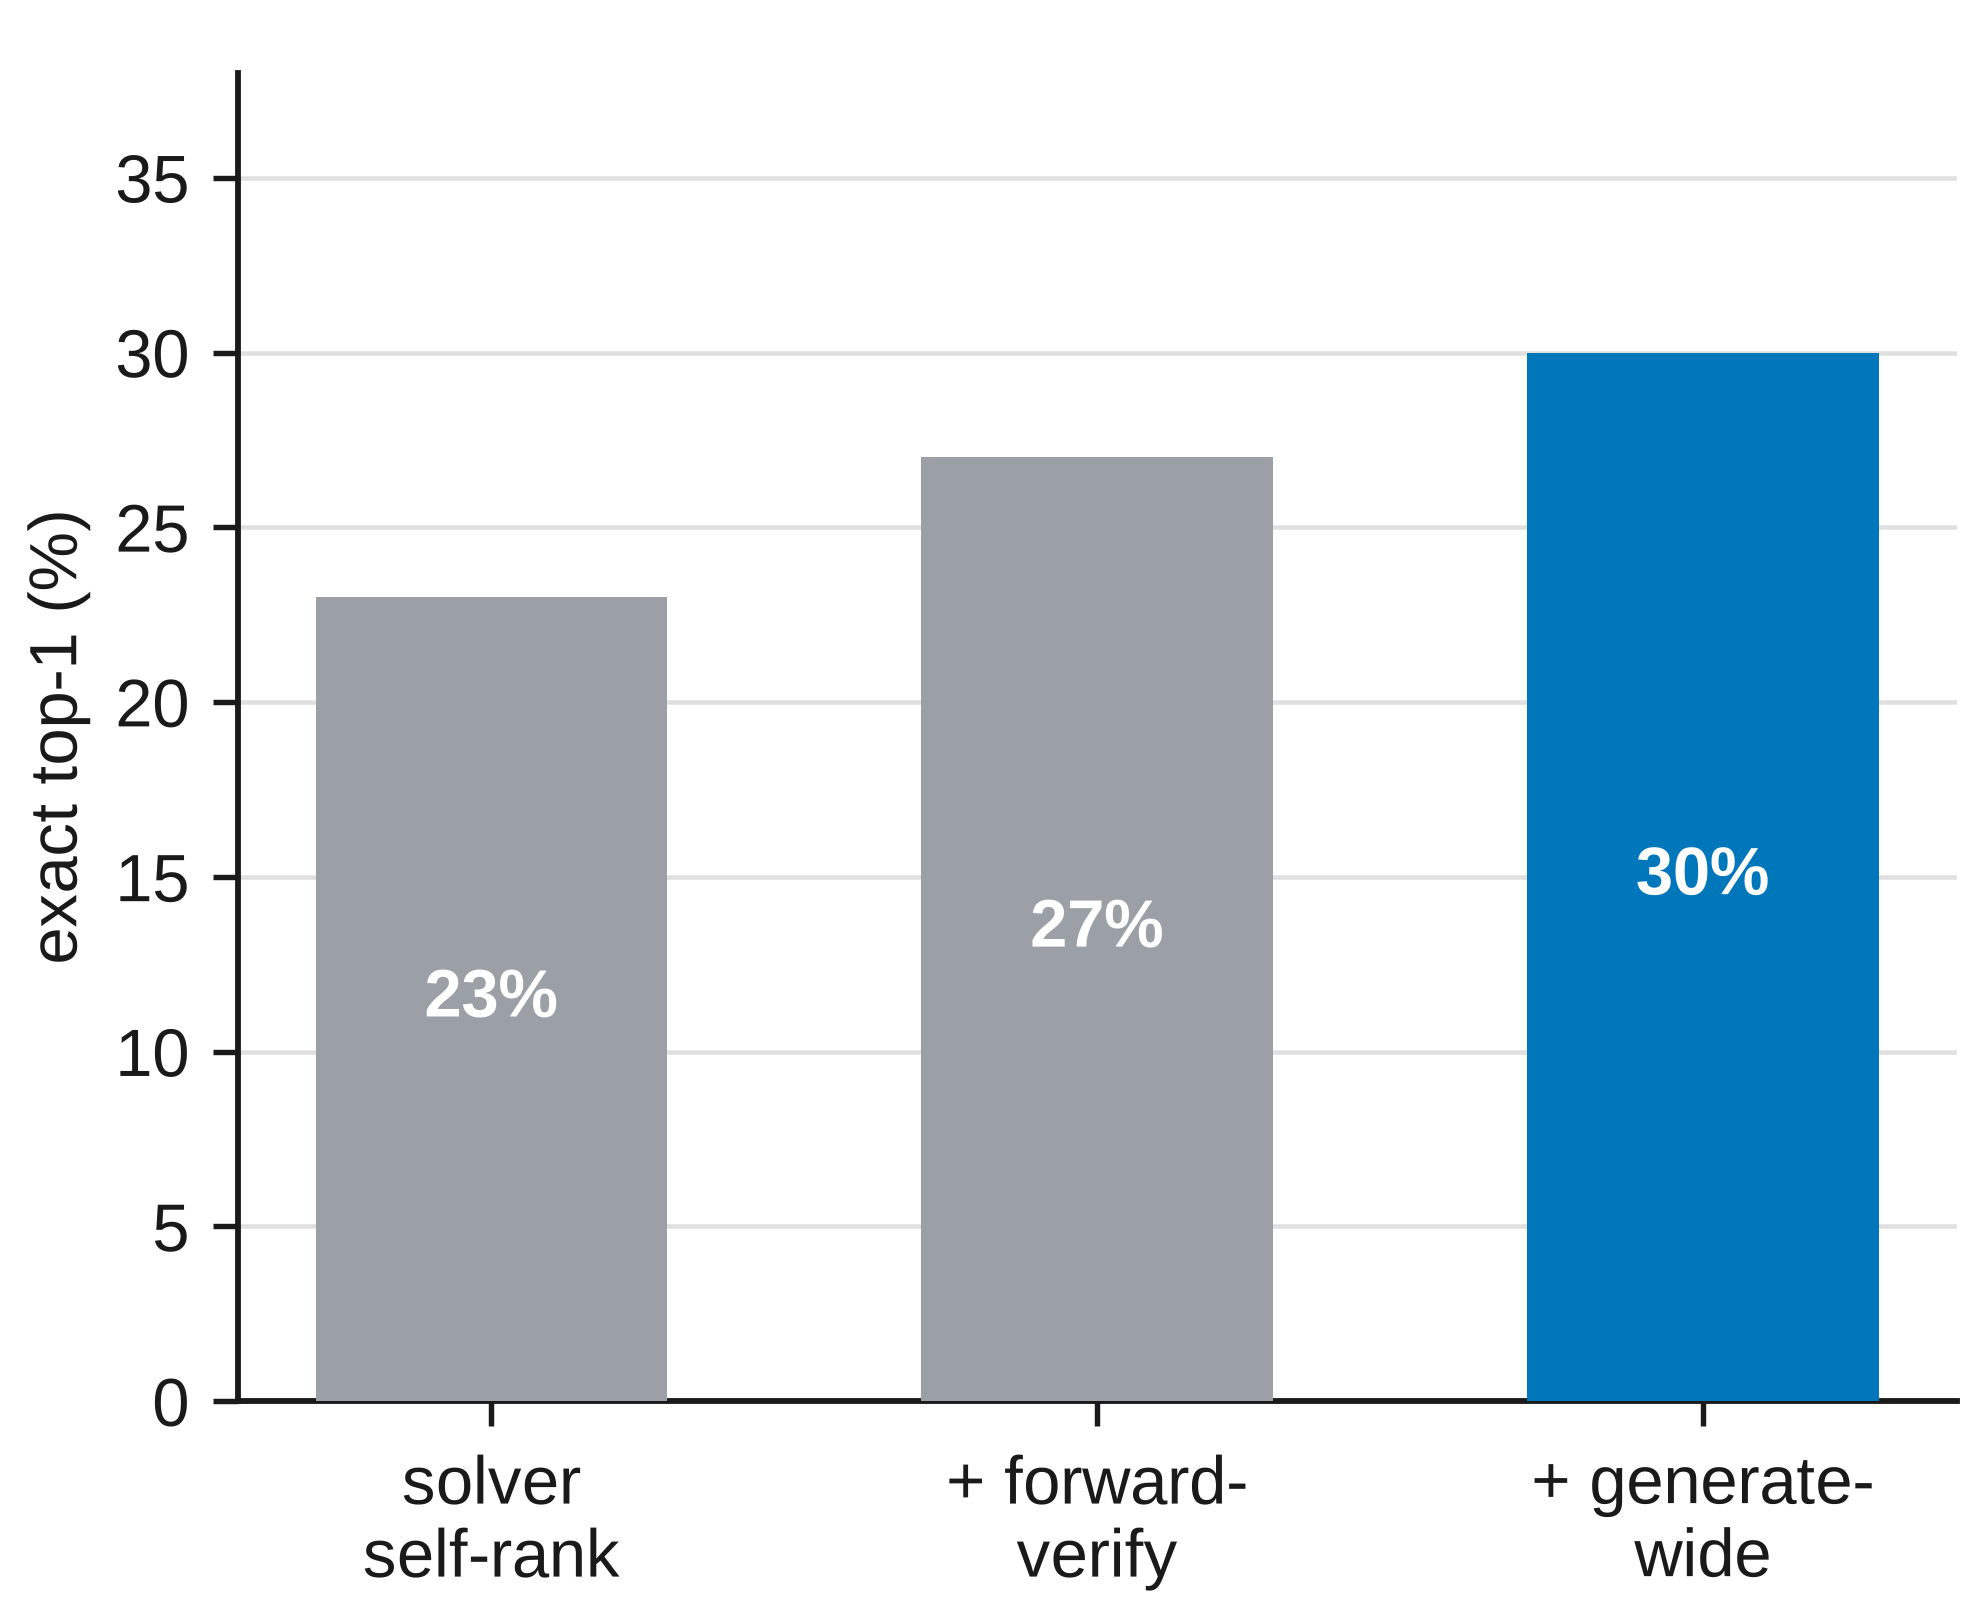
\includegraphics[width=0.52\linewidth]{fig3_method.png}
  \caption{Inference ladder on the 60-compound arm: 23\% $\to$ 27\% $\to$ 30\% top-1.
  Generate-wide lifts recall (32\% $\to$ 42\%); the wall is proposal, not ranking.}
  \label{fig:fig3-method}
\end{figure}

\paragraph{Non-LLM verifiers.}
On the same candidate sets, a HOSE-style lookup ties self-ranking; a modest GNN reaches
59/65 (91\%) vs the LLM verifier's 58/65 (89\%) --- directional.
Deranging observed $^{13}$C pairings collapses precision ($p{=}0.001$).
A small IRexp-fine-tuned generator pooled with Claude lifts locked-slice recall 33.5\% $\to$ 54.1\% and
top-1 28.4\% $\to$ 35.1\% (McNemar $p{=}0.015$), showing the wall is a property of
\textbf{training-free elicitation}, not of the task.

\subsection{Decomposition across published literature}
\label{sec:literature}

Any system reporting top-1 $= a$ and top-$k = b$ implies recall $\geq b$ and conditional
precision $\leq a/b$.
Applying this to published figures (\texttt{scripts/literature\_decomposition.py}):

\begin{table}[ht]
\caption{Selected literature decomposition rows (connectivity-scored or as published).}
\label{tab:lit-decomp}
\centering
\scriptsize
\setlength{\tabcolsep}{3pt}
\begin{tabular}{@{}p{2.6cm}p{2.4cm}rrrr@{}}
\toprule
system & data ($n$) & top-1 & top-$k$ ($k$) & recall & prec. \\
\midrule
this work, solver alone & literature (300) & 39.3\% & 44.3\% (3) & 44.3\% & 88.7\% \\
this work + forward-verify & literature (194) & 29.9\% & 33.5\% (3) & 33.5\% & \textbf{89.2\%} \\
NMR-Solver~\citep{jin2025nmrsolver} & literature (450) & 52.9\% & 67.3\% (10) & $\geq$67.3\% & $\leq$78.6\% \\
NMRAgent~\citep{fang2026nmragent} & literature (450) & 61.6\% & 70.0\% (10) & $\geq$70.0\% & $\leq$88.0\% \\
Espejo Morales~\citep{espejo2026agentic} & education (236) & 80.9\% & 90.0\% (5) & $\geq$90.0\% & $\leq$89.9\% \\
Espejo Morales~\citep{espejo2026agentic} & industrial (34) & 20.6\% & 29.1\% (5) & $\geq$29.1\% & $\leq$70.9\% \\
Alberts, 6--13 atoms~\citep{alberts2025benchmarks} & NIST IR (3,455) & 63.8\% & 84.0\% (10) & 84.0\% & 75.9\% \\
SpecX, scaffold split~\citep{xiang2026specx} & simulated (99,439) & 29.7\% & 50.6\% (10) & 50.6\% & 58.7\% \\
\bottomrule
\end{tabular}
\end{table}

\textbf{Three groups changed only the data}, and recall carried \textbf{68\%} (NMR-Solver
simulated $\to$ real), \textbf{70\%} (SpecX random $\to$ scaffold) and \textbf{83\%}
(Espejo education $\to$ industrial) of each collapse.
Recall binds where spectra are real and heterogeneous; ranking dominates on simulated or
single-library data.
The solver-alone precision column on $n{=}300$ is self-ranking (118/133); the
forward-verify row is the instrumented $n{=}194$ slice (58/65) --- not interchangeable.

\subsection{Pre-registered expansion, pooled headline, and scale roadmap}
\label{sec:expansion}

The $n{=}300$ headline is the pre-registered pool of the locked 194 and a 106-compound
expansion draw (Table~\ref{tab:slices}; Appendix Tables~\ref{tab:expansion},~\ref{tab:clean295}).
Five $^{13}$C-overread flags (R12, R22, R25, R82, R91) stay in the 300; validate-clean is
116/295 (39.3\%) top-1 / 130/295 (44.1\%) recall.
The expansion slice is easier (59.4\% vs 28.4\% top-1) --- disclosed, not hidden.
A Fable arm is incomplete (68/106; not scored; never pooled).
Figure~\ref{fig:fig-wall} and Table~\ref{tab:fverify} remain the $n{=}194$ instrumented
forward-verified diagnosis; expansion-106 fverify was \textbf{not} run.

\paragraph{Scale roadmap / larger blind round.}
A second pre-registered draw toward $n{\approx}500$ (230 compounds; 115/115 simple/complex;
six $^{13}$C-overread flags known \emph{before} any solve) now has \textbf{230/230} Opus
deposits and a frozen 690-candidate file.
Scoring is \textbf{deferred}: the answer key is withheld, no top-1 or recall exists, and
forward-verify was not run on this round.
Those deposits used a thinking-tier consumer arm and are not interchangeable with the
no-thinking $n{=}300$ protocol until scored under a declared contract.
This round is \textbf{not} pooled into the headline and is not a wall figure.

\section{Discussion}
\label{sec:discussion}

Frontier LLMs are \textbf{good verifiers} ($\approx$89\% conditional precision on the
$n{=}194$ instrumented slice) and \textbf{weak proposers} (44\% generation recall on
$n{=}300$; 34\% on the instrumented 194) on real literature peak lists --- propose $\gg$
verify, not the reverse.
The primary research contribution is the \textbf{benchmark + stage decomposition +
contamination/cross-vendor diagnosis}, not a solved elucidator and not a Data Descriptor
for IRexp.
The expansion slice scored higher than the locked 194 (Section~\ref{sec:expansion}); pooling
does not erase that gap.
The $n{\approx}500$ deposits do not yet change any scored number.

\paragraph{Reporting contract.}
External work on IRSpectra-Bench should deposit ranked SMILES under the released protocol and
report, at minimum: (i) top-1 constitution, (ii) generation recall, (iii) verification
precision $|$ recall, with bootstrap CIs and candidate budget.
Top-1 alone conflates the two stages.
Nonsignificant ladder gains (forward-verification vs self-ranking, $p{=}0.55$; generate-wide
top-1, $p{=}0.34$) should be cited as \textbf{diagnostic}, not as accuracy advances.
Corpus-reweighted top-1 (\textbf{26.5\%} on the validate-clean subset) is the better estimate
for an arbitrary literature draw.
Training is not foreclosed: IRexp fine-tuning lifts recall to 54\%.
Those gains compound with open experimental data, honest benchmarks, and inference scaffolding that
transfers to each new model.

\subsection{Implications for agentic elucidation}
\label{sec:agentic}

The diagnosis implies an \textbf{asymmetric pipeline}, not another verifier stacked on a thin
pool.
Proposal is the expensive stage: diversity, tool-use into enumeration / database search /
formula-constrained decode, or generate-wide sampling that actually enlarges the pool.
Verification is cheap: once the true constitution is proposed, training-free
forward-verification selects it $\approx$89\% of the time on the instrumented $n{=}194$
slice (58/65).
Spending the budget on a second ranker cannot recover the 129/194 compounds that were never
proposed.

IR-Agent-style table-interpretation and retrieve tools~\citep{noh2025iragent} are complementary
\emph{feature} agents --- they improve how a spectrum is read and how a given pool is
re-ranked.
MolQuest- and Espejo-style architecture search~\citep{han2026molquest,espejo2026agentic}
still needs this stage contract: a better reader that does not change
$P(\text{true}\in\text{pool})$ cannot move top-1 on a recall-bound bench.
The next ICLR-relevant agent is a \textbf{proposer}, not a second verifier:
formula-constrained generators, fragment assembly, and search that change that probability.
We are \textbf{not} shipping another ChemCrow-for-IR or a SpectraLLM-style fine-tune:
the bench is a reporting contract so external agents can be compared honestly on the same
object.
Multi-modal agents raise recall only if they enlarge the pool.
Training on open experimental corpora (IRexp as the pointer, not this paper's object) is the
one intervention we have already seen move recall (33.5\% $\to$ 54.1\% on the locked slice).
Nonsignificant ladder steps are \textbf{diagnostic}, not accuracy claims
(forward-verification vs self-ranking McNemar $p{=}0.55$; generate-wide top-1 $p{=}0.34$):
re-ranking is the wrong primary bet and does not license a solved-elucidator headline.

\section{Limitations}
\label{sec:limitations}

Scoring is mechanical; solver runs were transcript-audited for zero ground-truth access.
\textbf{(i) Consumer harness.} Claude Opus via consumer subscription; no model snapshot,
temperature, seed, or thinking tier. Exact inference is not reproducible; scoring is.
Batch instruction text was not captured --- only per-compound payloads are released.
We do \textbf{not} recommend thinking-high follow-ups as a path to a method result.
\textbf{(ii) Pretraining contamination} is bounded by formula-only (23\% $\to$ 5\%) and flat
recency but \textbf{not excluded}; verbatim spectral strings from PMC in the prompt remain a
retrieval confound.
\textbf{(iii) Object type, formula and scoring.} Band/shift lists, not raw traces; formula
supplied (as from HRMS) --- absolute accuracies are not interchangeable with no-formula
systems. Headline metrics score constitution; with stereochemistry, top-1 is 93/295 (31.5\%)
on the validate-clean subset.
\textbf{(iv) Statistical honesty.} Forward-verification vs self-ranking unresolved ($p{=}0.55$);
generate-wide top-1 likewise ($p{=}0.34$). Four-model comparison at $n{=}24$ underpowered for
adjacent ranks with disclosed protocol asymmetry. The inference ladder \textbf{diagnoses a
bottleneck}; it is not a demonstrated accuracy advance.
\textbf{(v) No method SOTA chase.} SpectraLLM, IR-Agent, Spectro, NMIRacle, Alberts IR
transformers and CASE were \textbf{not scored} on IRSpectra-Bench. The contribution is the
bench and the proposal$\ll$verification split, not a claim that an off-the-shelf LLM beats
trained elucidators.
\textbf{(vi) Expansion difficulty gap; fverify not on 106 or 230.} Expansion top-1 is 59\% vs 28\%
on the locked 194; pooling to $n{=}300$ does \textbf{not} hide that gap
(Table~\ref{tab:slices}). Figure~\ref{fig:fig-wall} and 58/65 are the locked $n{=}194$
instrumented slice; forward-verify was not run on the 106 or on the 230-compound
$n{\approx}500$ deposits. The $n{\approx}500$ round is deposited (230/230) and
\textbf{unscored} --- no top-1 --- and used a thinking-tier consumer arm, so it is not a
no-thinking replication. Headline $n{=}300$ is Claude Opus generation (no thinking
tier); four-vendor replication is on 60 compounds; candidate budgets differ.
A Fable expansion arm is incomplete (68/106) and is not pooled.
\textbf{(vii) Deferred arms.} Expert-chemist audit formally deferred (not run).
Leave-one-modality-out abandoned. Extraction-recall human audit of the mining parser is
deferred to the \textit{Scientific Data} companion.
\textbf{(viii) Scope.} Battery subset uses literature electrolyte chemistry, not operando
spectra; single-sample scoring per compound; organic literature bias of PMC-OA sources.
Short answers to the same attacks are collected in Appendix~\ref{app:faq}.

\section{Conclusion}
\label{sec:conclusion}

IRSpectra-Bench makes LLM structure elucidation from literature peak lists \textbf{measurable
and decomposable}.
On the pooled generation cohort ($n{=}300$), a frontier LLM recovers 39\% top-1 and 44\%
generation recall; corpus-reweighted top-1 is 27\%.
Propose $\gg$ verify: generation recall --- not verification --- binds end-to-end accuracy
(forward-verified on the locked $n{=}194$ slice); the diagnosis replicates across
vendors and is recovered from published top-$k$ figures.
We release frozen predictions and a mechanical scorer so others can report the same three
numbers.
The band-list resource behind the bench is documented separately as a
\textit{Scientific Data} Data Descriptor (in preparation)~\citep{yabbarov2026irexp}.

\section*{AI use statement}
Frontier LLMs were used as \textbf{experimental solvers} under the consumer harness in
Sections~\ref{sec:setup}--\ref{sec:results} (Claude Opus on the headline cohort; three
other vendor families on the 60-compound arm), not as a substitute for author analysis,
scoring, or claim-checking.
Inference used no thinking tier and no pinned model snapshot.
We did not use generative AI to invent or alter reported metrics.
Generative tools assisted manuscript editing and formatting; the authors reviewed the text
and take responsibility for all claims, including any AI-assisted wording.

\section*{Ethics statement}
This work evaluates publicly available open-access literature peak lists and commercial LLM
APIs under consumer terms.
No human-subject data.
We do not claim clinical or regulatory readiness for automated elucidation.
Licensing of redistributed numeric extractions is documented in the companion Data Descriptor
and dataset notices (PMC-OA terms are mixed --- not uniformly CC-BY; Chemotion is CC-BY-SA).

\section*{Reproducibility statement}
Every training-free number regenerates from released questions, answers, frozen predictions
and scripts in the code release.
The sampler, InChIKey scorer and forward-verification harness are scripted end-to-end.
Consumer-harness inference cannot be bit-exact replayed (Section~\ref{sec:limitations});
distributional agreement is the intended claim.
Fine-tuning against the bench should use \texttt{data/train\_no\_bench.jsonl.gz} so benchmark
InChIKeys are withheld.

\enlargethispage{5\baselineskip}
\section*{Acknowledgements}
We acknowledge support from the Natural Sciences and Engineering Research Council of Canada (NSERC) through a CREATE training program. Institutional details and named funding references are omitted for double-blind review and will be restored in the camera-ready version.
\bibliography{references}
\bibliographystyle{iclr2027_conference}

\appendix

\section{Dataset pointer (IRexp)}
\label{app:dataset}

IRexp is \textbf{not} re-described here as a Data Descriptor.
During double-blind review, the commercial redistributable pool is available from an anonymised review copy (no author-identifying host):
\begin{itemize}
  \item Anonymised dataset copy: \url{https://anonymous.4open.science/r/peaklist-corpus-review-10C4/}
  \item Companion manuscript: anonymised \textit{Scientific Data} Data Descriptor (in preparation)~\citep{yabbarov2026irexp}
\end{itemize}
Named archival hosting will replace the review copy in the camera-ready version.
File schema and aggregate counts ship with that copy (\texttt{SCHEMA.md}, \texttt{data/}).

Benchmark construction details beyond Section~\ref{sec:benchmark} (spectral validation
filters, prompt-leakage audit, electrolyte SMARTS) ship with the code release and the
companion Data Descriptor~\citep{yabbarov2026irexp}; they are not re-presented here.

\section{Reviewer FAQ}
\label{app:faq}

These answers restate Limitations~\ref{sec:limitations}; they add no new metrics.

\textbf{Why is top-1 39\% if the wall figure looks worse?}
Headline generation is $n{=}300$ (118/300 top-1; 133/300 recall).
Figure~\ref{fig:fig1}c and Figure~\ref{fig:fig-wall} are the locked $n{=}194$
forward-verified slice (58/7/129). Do not read the wall as a pooled $n{=}300$
diagnosis.

\textbf{Is the expansion hidden in the pool?}
No. Expansion top-1 is 59\% vs 28\% on the locked 194 (Table~\ref{tab:slices}).
That gap is a result.

\textbf{Where is forward-verify on the 106?}
Not run. Conditional 89\% (58/65) is $n{=}194$ only.
Do not invent a pooled $n{=}300$ wall.

\textbf{Where is the $n{\approx}500$ top-1?}
Nowhere. A 230-compound blind round is deposited (230/230; 690 candidates);
scoring is deferred (key withheld). Deposit counts are not accuracy.
Headline stays $n{=}300$. Those deposits used a thinking-tier arm and are not
interchangeable with the no-thinking protocol.

\textbf{Consumer harness / no snapshot / no thinking tier?}
Correct and intentional for the scored headline. Scoring of frozen deposits is
reproducible; inference is not bit-exact. We do not recommend thinking-high
experiments as a revision path for a method result.

\textbf{Why no SpectraLLM / IR-Agent / CASE SOTA table?}
Different objects (simulated or NIST IR; trained agents; exhaustive enumerators).
None is scored on this bench. The paper is a stage diagnosis, not a method race.

\textbf{Is IRexp a second ICLR paper?}
No. IRexp is a companion resource pointer (Appendix~\ref{app:dataset};
Figure~\ref{lst:payload}).
Corpus construction belongs in the \textit{Scientific Data} descriptor.

\section{Extended tables and figures}
\label{app:extended}

This conference version keeps the protocol plate
(Figure~\ref{fig:fig1}), chemistry space
(Figure~\ref{fig:fig-chemspace}), Listing~1 payload (Figure~\ref{lst:payload}),
robustness (Figure~\ref{fig:fig-robustness}), the
forward-verification mechanism (Figure~\ref{fig:fig-mechanism}), and the inference
ladder (Figure~\ref{fig:fig3-method}).
The diagnosis wall on the $n{=}194$ instrumented slice is repeated below
(Figure~\ref{fig:fig-wall}) so the lead figure is not the only copy.
Additional archive plates are omitted here; they do not change the pooled $n{=}300$
generation headline or the $n{=}194$ instrumented wall.

\begin{figure}[h]
  \centering
  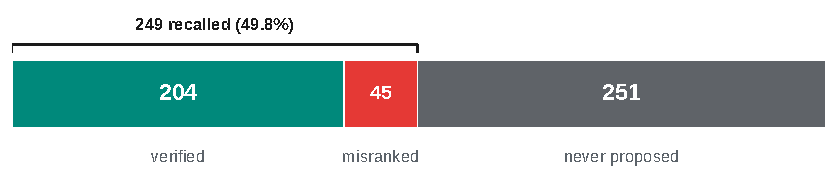
\includegraphics[width=0.92\linewidth]{fig_wall.pdf}
  \caption{Diagnostic wall: \textbf{locked $n{=}194$ instrumented slice}
  (58 verified / 7 mis-ranked / 129 never proposed).
  Expansion-106 has no forward-verify; this is \textbf{not} a pooled $n{=}300$ wall.
  Headline generation recall is 133/300.
  Never-proposed cases bind top-1 despite 89\% conditional precision (58/65).
  Same slice as Figure~\ref{fig:fig1}c.}
  \label{fig:fig-wall}
\end{figure}

\begin{table}[h]
\caption{Locked $n{=}194$ cases from released candidate files.
$^{13}$C chamfers in ppm; Tanimoto Morgan $r{=}2$. IDs are locked-round labels.}
\label{tab:cases}
\centering
\scriptsize
\setlength{\tabcolsep}{3.5pt}
\begin{tabular}{@{}lp{2.15cm}p{8.75cm}@{}}
\toprule
mode & id / formula & what failed \\
\midrule
\textbf{Proposal miss} &
main-R06 / C$_{29}$H$_{30}$FNO$_{2}$ &
True acridinedione never in the 3-candidate pool (Tanimoto-0.90 regioisomer: 4-fluorophenyl/phenyl swapped).
IR 1641, 1510~cm$^{-1}$; $^{13}$C 195.7. Verifier unused. \\
\textbf{Verify-save} &
v3-R25 / C$_{10}$H$_{14}$N$_{2}$O &
True 2-pyridyl picolinamide at self-rank 3; self-rank 1 is 3-pyridyl.
Forward-verify recovers (chamfer 0.42 vs 1.30~ppm). IR 1679~cm$^{-1}$.
Fig.~\ref{fig:fig-mechanism}. \\
\textbf{Verify-fail} &
v3-R26 / C$_{14}$H$_{11}$N$_{3}$O$_{3}$ &
True 3-nitrophenyl dihydroquinazolinone in pool (self-rank 2); 2-nitro ranked first.
Chamfer 1.35 vs 1.36~ppm. IR 1652, 1530, 1352~cm$^{-1}$. \\
\bottomrule
\end{tabular}
\end{table}

\begin{table}[h]
\caption{Expansion round (Claude Opus, InChIKey-14). Five $^{13}$C-overread flags stay in
the $n{=}300$ headline; validate-clean $n{=}295$ in Table~\ref{tab:clean295}.
Incomplete Fable arm (68/106) is never pooled.}
\label{tab:expansion}
\centering
\begin{tabular}{@{}lrr@{}}
\toprule
 & all ($n{=}106$) & clean ($n{=}101$) \\
\midrule
top-1 & 63/106 (59.4\%) & 61/101 (60.4\%) \\
generation recall & 68/106 (64.2\%) & 65/101 (64.4\%) \\
\bottomrule
\end{tabular}
\end{table}

\begin{table}[h]
\caption{Validate-clean sensitivity ($n{=}295$; five $^{13}$C-overread flags excluded).
Same scorer as Table~\ref{tab:headline}; not the headline.}
\label{tab:clean295}
\centering
\scriptsize
\setlength{\tabcolsep}{3pt}
\begin{tabular}{@{}lrrr@{}}
\toprule
metric & overall ($n{=}295$) & simple ($n{=}147$) & complex ($n{=}148$) \\
\midrule
top-1 exact constitution & 116/295 (39.3\%) [34--45] & 59.2\% [51--67] & 19.6\% [14--26] \\
recovered (top-3) & 130/295 (44.1\%) [39--49] & 63.9\% [56--71] & 24.3\% [17--31] \\
scaffold-level (best Tanimoto $\geq 0.45$) & 64\% & 80\% & 48\% \\
mean best Tanimoto & 0.66 & 0.79 & 0.53 \\
\bottomrule
\end{tabular}
\end{table}

By size on $n{=}295$: 67.9\% top-1 at $\leq$15 heavy atoms, 42.8\% at 16--25, 16.7\% above 25
($n{=}53/152/90$).
Full InChIKey (stereo): 93/295 (31.5\%) top-1 [26--37], recall 108/295 (36.6\%) [31--42].
Corpus-reweighted (17.5\% simple / 82.5\% complex): top-1 \textbf{26.5\%} [21--32], recall
\textbf{31.3\%} [25--37].
Self-ranking precision $|$ recall: 116/130 (89.2\%).

\end{document}
